\documentclass[12pt, a4paper]{report}

\usepackage[T1]{fontenc}
\usepackage[utf8]{inputenc}
\usepackage[ngerman]{babel}
\usepackage{lmodern}
\usepackage{microtype}
\usepackage{rotating}
\usepackage{geometry}
\geometry{a4paper, margin=2.5cm}

% Mathematik
\usepackage{amsmath, amssymb, amsthm, mathtools}
\usepackage{siunitx}
\sisetup{locale=DE, per-mode=fraction}
\DeclareSIUnit{\year}{a}
\usepackage{physics}
\ExplSyntaxOn
\msg_redirect_name:nnn { siunitx } { physics-pkg } { none }
\ExplSyntaxOff

% Grafiken
\usepackage{graphicx}
\usepackage{float}
\usepackage{caption}
\usepackage{subcaption}
\usepackage{tikz}
\usetikzlibrary{arrows.meta, decorations.pathmorphing, decorations.pathreplacing, patterns,
                positioning, shapes.geometric, calc,
                backgrounds, matrix, fit, shadings,
                decorations.markings, decorations.text}

% Tabellen
\usepackage{booktabs}
\usepackage{array}
\usepackage{longtable}
\usepackage{multirow}
\usepackage{xcolor}

% Hyperlinks
\usepackage[hidelinks]{hyperref}
\usepackage{cleveref}
\usepackage{eurosym}

% Aufzählungen
\usepackage{enumitem}
\setlist[itemize,1]{label=--}

% ─── Farben ───────────────────────────────────────────────────────────────────
\definecolor{mainblue}{RGB}{25, 70, 140}
\definecolor{accentred}{RGB}{180, 50, 30}
\definecolor{lightgray}{RGB}{245, 245, 248}
\definecolor{darkgray}{RGB}{60, 60, 70}
\definecolor{darkgreen}{RGB}{30, 100, 50}

\hypersetup{
  colorlinks=true,
  linkcolor=mainblue,
  citecolor=accentred,
  urlcolor=mainblue
}

% Rahmenboxen
\usepackage{mdframed}

\newmdenv[linewidth=1.5pt, innerleftmargin=8pt, innerrightmargin=8pt,
          innertopmargin=6pt, innerbottommargin=6pt,
          skipabove=\medskipamount, skipbelow=\medskipamount]{wichtigframe}
\newenvironment{wichtig}[1][]{%
  \begin{wichtigframe}\sloppy%
  \ifx&#1&\else\textbf{#1}\par\smallskip\fi}{\end{wichtigframe}}

\newmdenv[linewidth=3pt, topline=false, bottomline=false, rightline=false,
          innerleftmargin=10pt, innerrightmargin=4pt,
          innertopmargin=4pt, innerbottommargin=4pt,
          skipabove=\medskipamount, skipbelow=\medskipamount]{ergebnisframe}
\newenvironment{ergebnis}[1][]{%
  \begin{ergebnisframe}\sloppy%
  \ifx&#1&\else\textbf{#1}\par\smallskip\fi}{\end{ergebnisframe}}

\newmdenv[linewidth=0.6pt, innerleftmargin=8pt, innerrightmargin=8pt,
          innertopmargin=6pt, innerbottommargin=6pt,
          skipabove=\medskipamount, skipbelow=\medskipamount]{hinweisframe}
\newenvironment{hinweis}[1][]{%
  \begin{hinweisframe}\sloppy%
  \ifx&#1&\else\textbf{#1}\par\smallskip\fi}{\end{hinweisframe}}

% Theorem-Umgebungen
\theoremstyle{definition}
\newtheorem{theorem}{Satz}[section]
\newtheorem{lemma}[theorem]{Lemma}
\newtheorem{korollar}[theorem]{Korollar}
\newtheorem{definition}[theorem]{Definition}

\theoremstyle{remark}
\newtheorem{bemerkung}[theorem]{Bemerkung}
\newtheorem{beispiel}[theorem]{Beispiel}

% Abkürzungen
\newcommand{\rhoL}{\rho_{\text{L}}}
\newcommand{\cW}{c_{\text{W}}}
\newcommand{\Astirnfl}{A_{\text{Stirn}}}
\newcommand{\Aeinlass}{A_{\text{Einlass}}}
\newcommand{\vek}[1]{\boldsymbol{#1}}
\newcommand{\kB}{k_{\text{B}}}
\newcommand{\NA}{N_{\text{A}}}
\newcommand{\RE}{R_{\oplus}}
\newcommand{\ME}{M_{\oplus}}

\title{%
  \textbf{Induktionsfedern als \\aerodynamische Energiequelle}\\[6pt]
  \large Physikalische Analyse, Energiebilanz und Grenzen\\
  bei Kraftfahrzeugen und Satelliten im erdnahen Orbit
}
\author{Stephan Epp}
\date{27. März 2026}

% ─────────────────────────────────────────────────────────────────────────────
\begin{document}
% ─────────────────────────────────────────────────────────────────────────────

\maketitle
\tableofcontents
\newpage

% ─────────────────────────────────────────────────────────────────────────────
\chapter{Einleitung}
\label{chap:einleitung}
% ─────────────────────────────────────────────────────────────────────────────

Der steigende Energiebedarf moderner Kraftfahrzeuge und die strenger werdenden
CO\textsubscript{2}-Grenzwerte fordern die Entwicklung neuartiger Methoden zur
Energierückgewinnung. Eine viel diskutierte Klasse von Konzepten betrifft die
Nutzung des beim Fahren entstehenden \emph{Luftwiderstands} als sekundäre
Energiequelle. Im Zentrum dieser Arbeit steht das Konzept der
\textbf{Induktionsfeder} -- ein miniaturisierter schwingungsfähiger
Energiewandler, der in den Luftstrom eines fahrenden Fahrzeugs eingebracht
wird und kinetische Strömungsenergie in elektrische Energie umwandelt.

Parallel dazu stellt sich für Satelliten im \emph{erdnahen Orbit} (ca.\ 80
bis 400\,km Höhe) die Frage, ob der dort wirkende atmosphärische Restluft\-widerstand
als Energiequelle für Bord\-systeme genutzt werden kann. Insbesondere die
Orbitalhöhe von rund \SI{100}{\kilo\metre} -- die sogenannte \emph{Kármán-Linie}
als internationale Grenze zum Weltraum -- ist dabei von besonderem Interesse,
da hier die Luftdichte noch ausreichend groß ist, um merkliche aerodynamische
Kräfte zu erzeugen.

\begin{hinweis}[Abgrenzung zu anderen Konzepten]
  Die Induktionsfeder stellt keine völlig neue Erfindung dar: Verwandte
  Konzepte sind Piezo-Ernter (engl.\ \emph{Piezoelectric Energy Harvesters}),
  Winkelgetriebe-Generatoren und Vortex-Induced-Vibration-(VIV-)Wandler.
  Der Beitrag dieser Arbeit liegt in der \emph{systematischen physikalischen
  Modellierung}, der \emph{vollständigen Energiebilanz} sowie der
  \emph{formalen thermodynamischen Bewertung} aller Szenarien.
\end{hinweis}

\section{Historischer Hintergrund und verwandte Arbeiten}

Die Idee, kinetische Energie eines vorbeiströmenden Fluids mittels
schwingungsfähiger Körper in Elektrizität umzuwandeln, geht auf frühe
Untersuchungen zur \emph{Kármán'schen Wirbelstraße} zurück:

\begin{itemize}
  \item \textbf{von Kármán (1911):} Str\"omungsinstabilit\"aten hinter stumpfen
        K\"orpern f\"uhren zu periodisch abwechselnden Wirbelablösungen, die
        transversale Schwingungsanregungen erzeugen~\cite{karman1911}.
  \item \textbf{Strouhal (1878):} Quantitative Beschreibung der
        Wirbelfrequenz~\cite{strouhal1878}.
  \item \textbf{McKinney \& DeLaurier (1981):} Erste Studie zur Leistungsentnahme
        aus VIV-Schwingungen~\cite{mckinney1981}.
  \item \textbf{Anton \& Sodano (2007):} Übersichtsartikel über aerodynamische
        Piezo-Ernter~\cite{anton2007}.
  \item \textbf{Tang et al.\ (2009):} Aeroelastische Flatter-Ernter~\cite{tang2009}.
\end{itemize}

Im Bereich der Fahrzeuganwendungen wurde von mehreren Automobilherstellern
experimentiert:\ Bose, Toyota und Honda publizierten Studien zu
\emph{regenerativen Stoßdämpfersystemen}, die Fahrbahnunebenheiten nutzen.
Die Nutzung des \emph{Fahrtwinds} als Einlassstrom ist dagegen weniger
systematisch untersucht.

\section{Ziel}

Diese Untersuchung verfolgt folgende Ziele:

\begin{enumerate}[leftmargin=2em]
  \item \textbf{Physikalisches Modell:} Formale Herleitung der Leistungsgleichungen
        für Induktionsfedern im Strömungskanal eines Fahrzeugs.
  \item \textbf{Energiebilanz KFZ:} Vollständige Analyse der erntefähigen
        elektrischen Leistung bei vollständiger Frontflächenausnutzung
        (Breite \SI{1.8}{\metre} $\times$ Höhe \SI{0.4}{\metre}).
  \item \textbf{Satelliten-Szenario:} Berechnung der verfügbaren
        Luftwiderstandsleistung in \SI{100}{\kilo\metre} Orbitalhöhe.
  \item \textbf{Thermodynamische Grenzen:} Formaler Beweis, warum ein
        dauerhafter Eigenantrieb ausschließlich aus dem Luftwiderstand
        dem Ersten Hauptsatz der Thermodynamik widerspricht.
  \item \textbf{Legitime Anwendungen:} Identifikation der physikalisch
        realisierbaren Nutzung als \emph{Hilfsleistungsquelle}.
\end{enumerate}

Die Aussage dieser Arbeit ist, Induktionsfedern gewinnen elektrische Hilfsleistung aus dem Fahrtluftström (für Bordnetz, Beleuchtung, Klimatisierung). Sie können jedoch \emph{nicht} als Primärantrieb dienen, da dies die Energieerhaltung verletzen würde. Eine exakte Bilanzrechnung belegt dies.

% ─────────────────────────────────────────────────────────────────────────────
\chapter{Grundlagen der Aerodynamik}
\label{chap:aerodynamik}
% ─────────────────────────────────────────────────────────────────────────────

\section{Die Bernoulli-Gleichung}

Die Bernoulli-Gleichung für stationäre, inkompressible, reibungsfreie Strömungen
längs einer Stromlinie lautet:

\begin{equation}
  p + \frac{1}{2}\rhoL v^2 + \rhoL g z = \text{const}
  \label{eq:bernoulli}
\end{equation}

Dabei bezeichnen $p$ den Druck, $\rhoL$ die Luftdichte, $v$ die Strömungsgeschwindigkeit
und $z$ die Höhe. Der Term $\frac{1}{2}\rhoL v^2$ heißt \emph{dynamischer Druck}
$q$ und ist von fundamentaler Bedeutung für die Luftwiderstandsbeziehung:

\begin{equation}
  q = \frac{1}{2}\rhoL v^2
  \label{eq:dyn_druck}
\end{equation}

Für Fahrzeuggeschwindigkeiten bis \SI{200}{\kilo\metre\per\hour} ist die
Machzahl $Ma = v/v_{\text{Schall}} < 0.16$, womit die Inkompressibilitäts\-annahme
mit einem Fehler $< 1.3\,\%$ gerechtfertigt ist.

\section{Luftwiderstandskraft und -leistung}

Die Luftwiderstandskraft eines Körpers ist durch den dimensionslosen
\emph{$\cW$-Wert} (Luftwiderstandsbeiwert, engl.\ \emph{drag coefficient}
$c_D$) definiert:

\begin{equation}
  F_W = \cW \cdot \frac{1}{2}\rhoL v^2 \cdot \Astirnfl
  \label{eq:fw}
\end{equation}

Die zur Überwindung dieses Widerstands benötigte \emph{Antriebsleistung} ist:

\begin{equation}
  P_W = F_W \cdot v = \cW \cdot \frac{1}{2}\rhoL v^3 \cdot \Astirnfl
  \label{eq:pw}
\end{equation}

\begin{wichtig}[Kubische Geschwindigkeitsabhängigkeit]
  Gleichung~\eqref{eq:pw} zeigt: Die Luftwiderstandsleistung wächst mit der
  \emph{dritten Potenz} der Geschwindigkeit. Eine Verdopplung der Geschwindigkeit
  (z.\,B.\ von 65 auf 130\,km/h) veracht\-facht die Luftwiderstandsleistung.
  Dies hat erhebliche Konsequenzen sowohl für den Energiebedarf als auch für
  die potenzielle Ernteleistung der Induktionsfedern.
\end{wichtig}

Für einen typischen Serien-PKW mit $\cW = 0.28$ und $\Astirnfl = \SI{2.2}{\metre\squared}$:

\begin{align}
  P_W(50\text{ km/h})  &= 0.28 \cdot \tfrac{1}{2} \cdot 1.225 \cdot 13.9^3 \cdot 2.2 \approx \SI{1.01}{\kilo\watt} \label{eq:pw50}\\
  P_W(100\text{ km/h}) &= 0.28 \cdot \tfrac{1}{2} \cdot 1.225 \cdot 27.8^3 \cdot 2.2 \approx \SI{8.08}{\kilo\watt} \label{eq:pw100}\\
  P_W(130\text{ km/h}) &= 0.28 \cdot \tfrac{1}{2} \cdot 1.225 \cdot 36.1^3 \cdot 2.2 \approx \SI{17.8}{\kilo\watt} \label{eq:pw130}
\end{align}

\section{Rollwiderstand}

Der \emph{Rollwiderstand} eines Fahrzeugs (Reifenverformung, Lagerreibung) ist:

\begin{equation}
  F_R = \mu_R \cdot m \cdot g, \qquad P_R = F_R \cdot v = \mu_R \cdot m \cdot g \cdot v
  \label{eq:roll}
\end{equation}

Für typische Werte $\mu_R = 0.012$, $m = \SI{1500}{\kilo\gram}$:

\begin{equation}
  P_R(v) = 0.012 \cdot 1500 \cdot 9.81 \cdot v \approx 176.6 \cdot v \quad [\si{\watt}]
  \label{eq:pr_param}
\end{equation}

Der Schnittpunkt von $P_W$ und $P_R$ zeigt den Geschwindigkeitsbereich, bei dem
der Luftwiderstand die dominierende Verlustquelle wird:

\begin{equation}
  v^* = \left(\frac{2\mu_R m g}{\rhoL \cW \Astirnfl}\right)^{1/2}
      = \left(\frac{2 \cdot 0.012 \cdot 1500 \cdot 9.81}{1.225 \cdot 0.28 \cdot 2.2}\right)^{1/2}
      \approx \SI{62}{\kilo\metre\per\hour}
  \label{eq:v_kreuzung}
\end{equation}

Oberhalb von \SI{62}{\kilo\metre\per\hour} dominiert der Luftwiderstand.

\section{US-Standardatmosphäre}

Das mathematische Modell der Atmosphäre ist für die Satelliten-Berechnung essenziell.
Die US-Standardatmosphäre (USSA76) beschreibt die Dichte im Bereich 0 bis \SI{86}{\kilo\metre}
schichtweise; oberhalb \SI{86}{\kilo\metre} (Thermosphäre) wird ein vereinfachter
Exponentialabfall verwendet:

\begin{equation}
  \rhoL(h) =
  \begin{cases}
    1.225\left(1 - 2.2558 \times 10^{-5}\,h\right)^{4.2561} & 0 \le h \le \SI{11}{\kilo\metre} \\
    0.3639\,e^{-1.5788 \times 10^{-4}(h - 11\,000)} & 11 < h \le \SI{25}{\kilo\metre} \\
    \rho_{25} \cdot f_{\text{strat}}(h) & 25 < h \le \SI{47}{\kilo\metre} \\
    \rho_{86} \cdot e^{-\alpha_T (h - 86\,000)} & h > \SI{86}{\kilo\metre}
  \end{cases}
  \label{eq:ussa76}
\end{equation}

wobei $\alpha_T \approx 6.5 \times 10^{-5}\,\si{\per\metre}$ die Skalenhöhe der
Thermosphäre beschreibt. An der Kármán-Linie ($h = \SI{100}{\kilo\metre}$) ergibt
sich eine Luftdichte von:

\begin{equation}
  \rhoL(100\,\text{km}) \approx 5.6 \times 10^{-7}\,\si{\kilo\gram\per\cubic\metre}
  \label{eq:rho100}
\end{equation}

Dies entspricht einem Faktor $\approx 2.2 \times 10^{6}$ unterhalb der
Meeresspiegeldichte -- für die Widerstandsberechnung ist damit eine
Satellitenlösung mit großer Querschnittsfläche und hoher Orbitalgeschwindigkeit
erforderlich, um messbare Kräfte zu erzielen.

\begin{figure}[H]
  \centering
  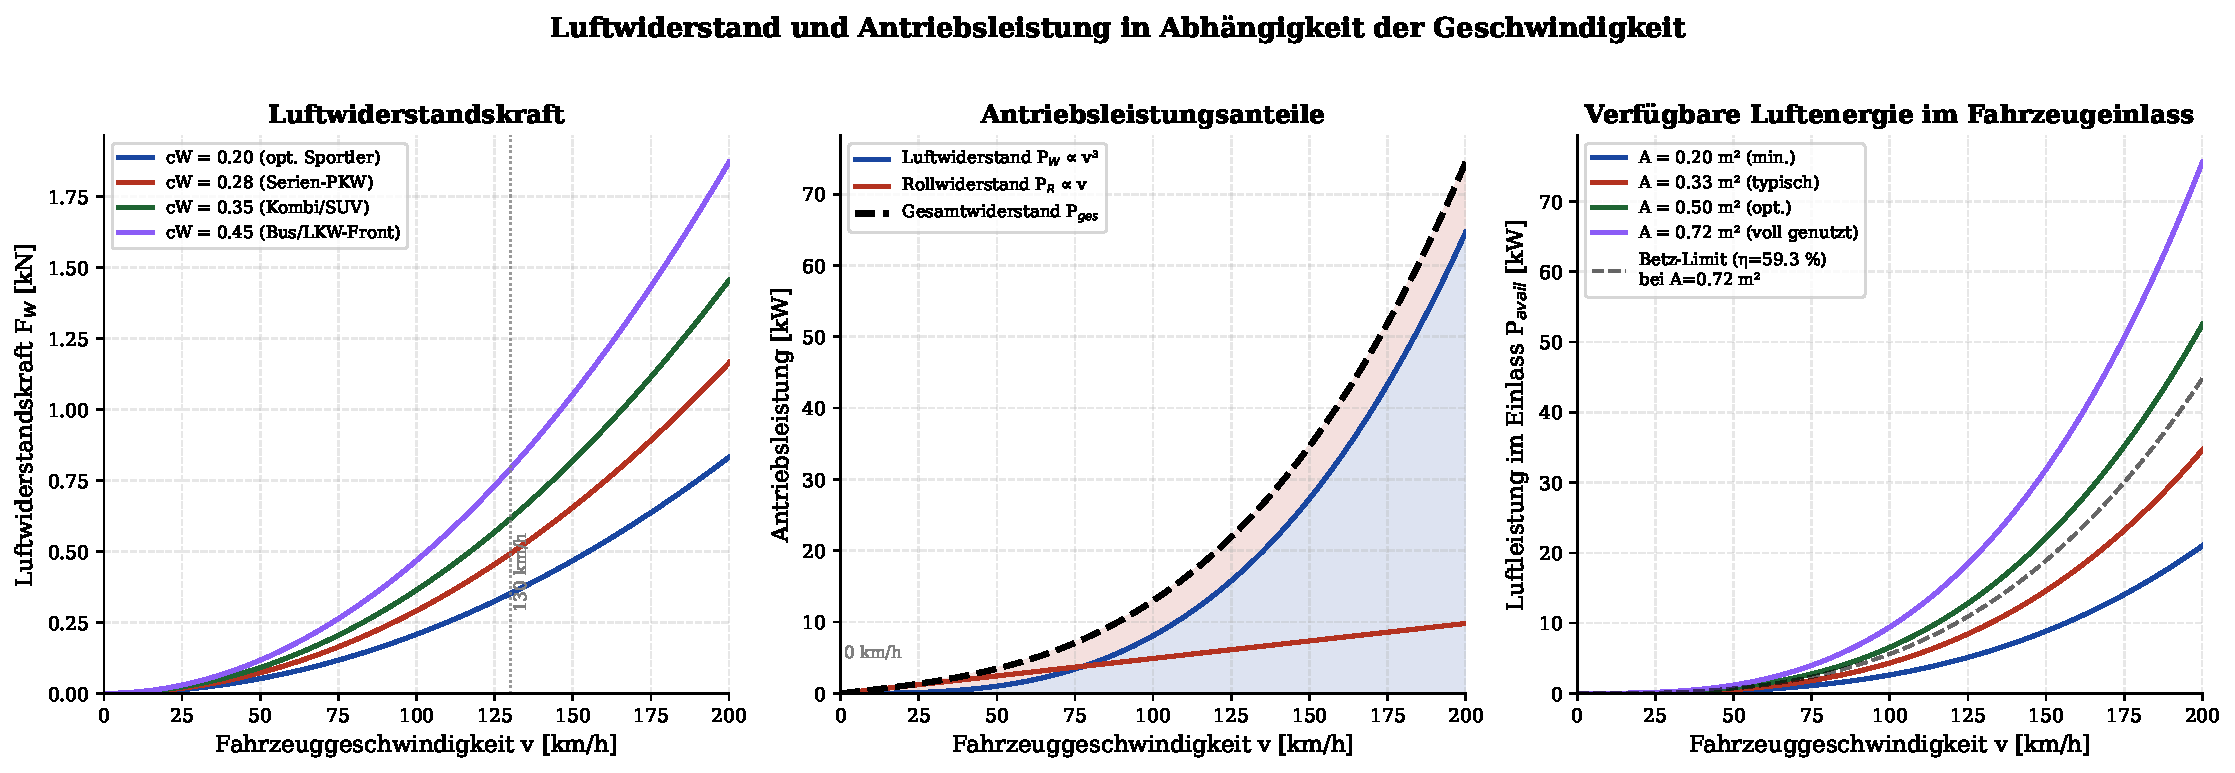
\includegraphics[width=\textwidth]{plots/plot1_luftwiderstand.pdf}
  \caption{%
    \textbf{Luftwiderstand und Antriebsleistung in Abhängigkeit der Fahrzeuggeschwindigkeit.}
    \textit{Links:} Luftwiderstandskraft für verschiedene $\cW \cdot A$-Produkte.
    Die stark nichtlineare (quadratische) Zunahme mit der Geschwindigkeit ist
    klar erkennbar; bei 200\,km/h übersteigt die Widerstandskraft für einen
    typischen SUV bereits $\SI{1}{\kilo\newton}$.
    \textit{Mitte:} Antriebsleistungsanteile (gestapelt): Luftwiderstand (blau)
    wächst kubisch, Rollwiderstand (rot) linear; ab ca.\ 62\,km/h dominiert der
    Luftwiderstand.
    \textit{Rechts:} Im Einlass verfügbare Luftleistung (kinetischer Fluss
    $\frac{1}{2}\rhoL v^3 A_{\text{Einlass}}$) für verschiedene
    Einlassflächen. Die gestrichelte Kurve zeigt das Betz-Limit ($\eta = 59.3\,\%$)
    für die vollständige Frontflächenausnutzung $A = \SI{0.72}{\metre\squared}$.
  }
  \label{fig:luftwiderstand}
\end{figure}

\section{Grenzschicht und turbulente Strömung}

Die charakteristische Reynoldszahl für einen Fahrzeugeinlass mit
Kanaldurchmesser $d = \SI{0.05}{\metre}$ bei $v = \SI{36}{\metre\per\second}$
(130\,km/h) ist:

\begin{equation}
  Re = \frac{v \cdot d}{\nu} = \frac{36 \cdot 0.05}{1.5 \times 10^{-5}} = 1.2 \times 10^5
  \label{eq:reynolds}
\end{equation}

Da $Re \gg Re_{\text{krit}} \approx 2300$, liegt vollständig turbulente Stömung vor.
Die \emph{Kármán'sche Wirbelstraße} hinter zylindrischen Hindernissen hat die
Strouhal-Frequenz:

\begin{equation}
  f_{\text{Kármán}} = St \cdot \frac{v}{d}, \qquad St \approx 0.20
  \label{eq:strouhal}
\end{equation}

Bei $v = 130\,\text{km/h} = 36.1\,\text{m/s}$ und $d = 0.05\,\text{m}$:
\begin{equation}
  f_{\text{Kármán}} = 0.20 \cdot \frac{36.1}{0.05} = \SI{144}{\hertz}
  \label{eq:f_karman_130}
\end{equation}

Diese Frequenz bestimmt die \emph{Resonanzauslegung} der Induktionsfedern,
wie in Kapitel~\ref{chap:federsystem} gezeigt wird.

% ─────────────────────────────────────────────────────────────────────────────
\chapter{Konzept und Physik der Induktionsfeder}
\label{chap:federsystem}
% ─────────────────────────────────────────────────────────────────────────────

\section{Mechanisches Grundmodell: Schwingender Körper im Fluidstrom}

Eine Induktionsfeder (IF) ist ein schwingungsfähiges Masse-Feder-Dämpfer-System,
das in einem Strömungskanal angebracht wird. Der Strömungsdruck versetzt die
Schwingmasse $m_s$ in Resonanzschwingungen, die elektromagnetisch oder
piezoelektrisch in elektrische Energie umgewandelt werden.

\begin{definition}[Induktionsfeder]
  Eine \emph{Induktionsfeder} ist ein mechanischer Resonator bestehend aus:
  \begin{itemize}
    \item einer Schwingmasse $m_s$ (typisch 10--100\,g),
    \item einer Rückstellfeder der Steifigkeit $k$,
    \item einem mechanischen (parasitären) Dämpfer $c_m$ (Reibung, Material),
    \item einem \emph{elektrischen Dämpfer} $c_e$ (Energieentnahme durch
          elektrisches Feld/Piezo).
  \end{itemize}
\end{definition}

Die Bewegungsgleichung bei harmonischer Anregung $F(t) = \hat{F}\sin(\omega t)$:

\begin{equation}
  m_s \ddot{x} + (c_m + c_e)\dot{x} + k x = \hat{F}\sin(\omega t)
  \label{eq:bewegungsgl}
\end{equation}

Die stationäre Lösung hat die Amplitude:

\begin{equation}
  \hat{X}(\omega) = \frac{\hat{F}/k}{\sqrt{\left(1 - \left(\frac{\omega}{\omega_0}\right)^2\right)^2
  + \left(\frac{(c_m + c_e)\,\omega}{k}\right)^2}}, \qquad
  \omega_0 = \sqrt{\frac{k}{m_s}}
  \label{eq:amplitude}
\end{equation}

\section{Elektrische Ausgangsleistung}

Die vom elektrischen Dämpfer $c_e$ entnommene Leistung ist die nutzbare
elektrische Leistung der Induktionsfeder:

\begin{equation}
  P_{\text{el}} = \frac{1}{2} c_e \omega^2 \hat{X}^2(\omega)
  \label{eq:p_el}
\end{equation}

Einsetzen von Gleichung~\eqref{eq:amplitude}:

\begin{equation}
  P_{\text{el}}(\omega) = \frac{\hat{F}^2}{2k^2} \cdot
  \frac{c_e\,\omega^2}{\left(1-\left(\frac{\omega}{\omega_0}\right)^2\right)^2
  + \left(\frac{(c_m+c_e)\omega}{k}\right)^2}
  \label{eq:p_el_full}
\end{equation}

\begin{theorem}[Optimaler elektrischer Dämpfer]
  \label{thm:opt_daempfer}
  Bei Betrieb in Resonanz ($\omega = \omega_0$) wird $P_{\text{el}}$ maximiert bei:
  \begin{equation}
    c_e^* = c_m
    \label{eq:ce_opt}
  \end{equation}
  Die maximale Leistung beträgt dann:
  \begin{equation}
    P_{\text{el,max}} = \frac{\hat{F}^2}{8\,c_m^2\,\omega_0^2}\cdot\frac{1}{m_s} \cdot m_s \omega_0^2
    = \frac{\hat{F}^2}{8\,c_m\,\omega_0}
    \label{eq:p_el_max}
  \end{equation}
\end{theorem}

\begin{proof}
  Bei $\omega = \omega_0$ vereinfacht sich Gl.~\eqref{eq:p_el_full} zu:
  \begin{equation}
    P_{\text{el}}(\omega_0) = \frac{\hat{F}^2}{2m_s^2\omega_0^4} \cdot
    \frac{c_e}{(c_m + c_e)^2}
  \end{equation}
  Ableitung nach $c_e$ und Nullsetzen:
  \begin{equation}
    \frac{\dd P_{\text{el}}}{\dd c_e} = \frac{\hat{F}^2}{2m_s^2\omega_0^4}
    \cdot \frac{(c_m + c_e)^2 - 2c_e(c_m + c_e)}{(c_m + c_e)^4} = 0
  \end{equation}
  Zähler null: $c_m + c_e - 2c_e = 0 \implies c_e = c_m$. 
\end{proof}

\section{Resonanzauslegung für Fahrtwind}

Die Eigenfrequenz der Induktionsfeder muss auf die Kármán-Wirbelfrequenz
(Gl.~\eqref{eq:strouhal}) abgestimmt werden:

\begin{equation}
  \omega_0 = 2\pi f_{\text{Kármán}} = 2\pi \cdot St \cdot \frac{v}{d}
\end{equation}

Die passende Federsteifigkeit bei gegebener Schwingmasse $m_s$:

\begin{equation}
  k^* = m_s \omega_0^2 = m_s \left(2\pi \cdot 0.20 \cdot \frac{v}{d}\right)^2
    = m_s \cdot \frac{4\pi^2 \cdot 0.04 \cdot v^2}{d^2}
  \label{eq:k_opt}
\end{equation}

\begin{beispiel}[Auslegung für 100\,km/h]
  Mit $m_s = \SI{0.05}{\kilo\gram}$, $d = \SI{0.05}{\metre}$, $v = 27.8\,\text{m/s}$:
  \begin{align}
    f_{\text{Kármán}} &= 0.20 \cdot \frac{27.8}{0.05} = \SI{111}{\hertz} \\
    k^* &= 0.05 \cdot (2\pi \cdot 111)^2 = 0.05 \cdot (697.4)^2 \approx \SI{24\,300}{\newton\per\metre}
  \end{align}
  Eine solche Feder ist technisch gut realisierbar (z.\,B.\ Stahl-Blattfeder).
\end{beispiel}

\begin{figure}[H]
  \centering
  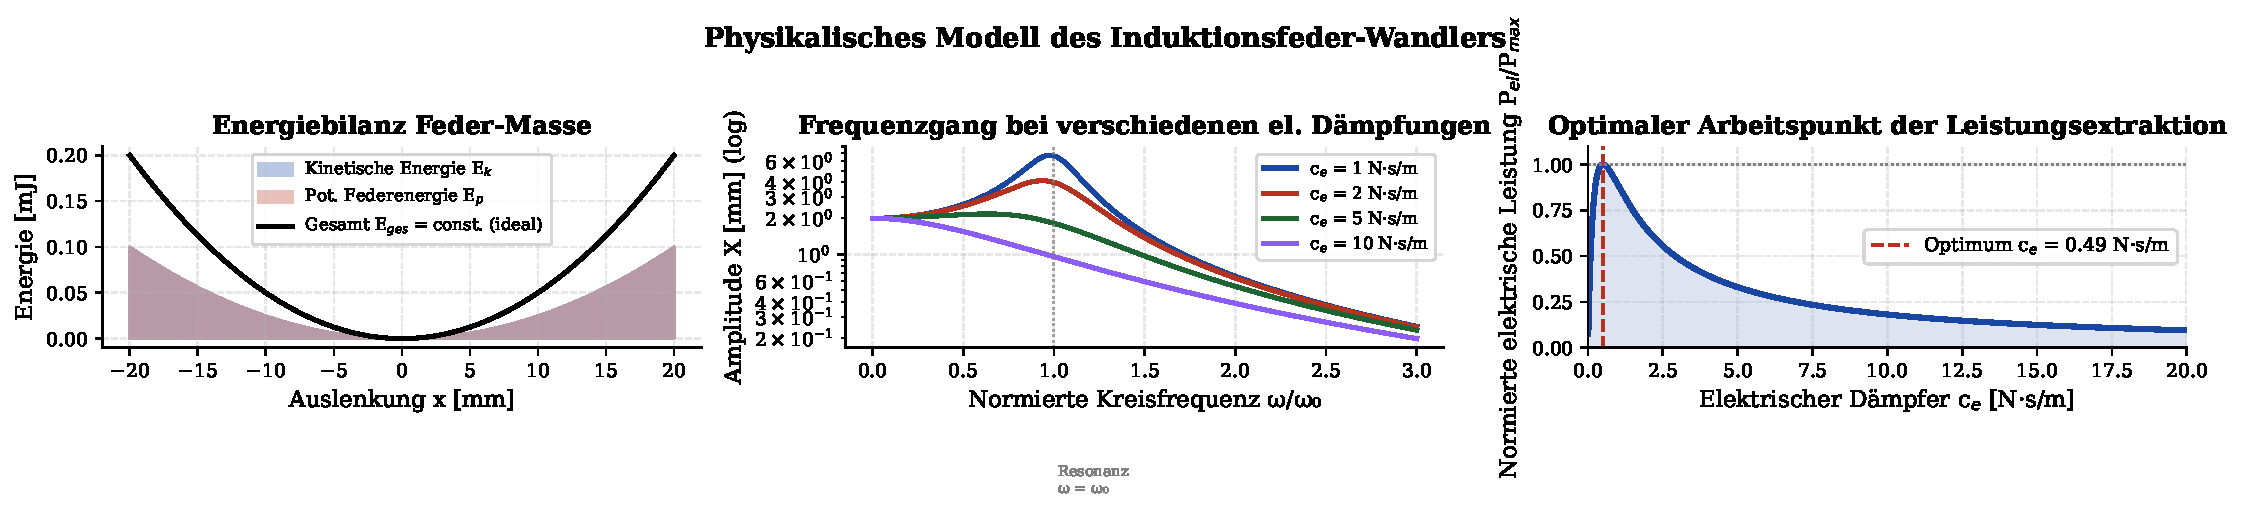
\includegraphics[width=\textwidth]{plots/plot2_federsystem.pdf}
  \caption{%
    \textbf{Physikalisches Modell der Induktionsfeder.}
    \textit{Links:} Energiebilanz des Feder-Masse-Systems: kinetische
    Energie (blau) und potentielle Federenergie (rot) sind im idealen System
    konstant.
    \textit{Mitte:} Frequenzgang (Resonanzkurve) für verschiedene elektrische
    Dämpfer $c_e$. Bei zu kleinem $c_e$ schwingt das System zu stark, bei zu
    großem wird es überdämpft; das Optimum liegt bei $c_e = c_m$.
    \textit{Rechts:} Normierte elektrische Ausgangsleistung als Funktion des
    elektrischen Dämpfers -- deutliches Maximum bei $c_e^* = c_m \approx 2\,\text{N·s/m}$.
  }
  \label{fig:federsystem}
\end{figure}

\section{Elektromagnetischer Wandler: Faradaysches Induktionsgesetz}

Bei einem elektromagnetischen Wandler (Tauchspule oder Linearmotor-Prinzip)
gilt das Faraday'sche Induktionsgesetz:

\begin{equation}
  \mathcal{E} = -\frac{\dd\Phi}{\dd t} = B \cdot l \cdot \dot{x}(t)
  \label{eq:emk}
\end{equation}

Dabei ist $B$ die magnetische Flussdichte, $l$ die effektive Leiterlänge der
Spule und $\dot{x}$ die Schwinggeschwindigkeit. Die Leistung an einem
Lastwiderstand $R_L$:

\begin{equation}
  P_{\text{el}} = \frac{\mathcal{E}^2}{(R_L + R_i)^2} \cdot R_L
  = \frac{(Bl)^2 \dot{x}^2}{(R_L + R_i)^2} \cdot R_L
  \label{eq:p_el_em}
\end{equation}

Für $R_L = R_i$ (Leistungsanpassung):

\begin{equation}
  P_{\text{el,max}} = \frac{(Bl)^2 \dot{x}^2}{4 R_i}
  \label{eq:p_el_em_max}
\end{equation}

Der äquivalente elektrische Dämpfungskoeffizient des elektromagnetischen
Wandlers ist:

\begin{equation}
  c_e^{\text{EM}} = \frac{(Bl)^2}{R_L + R_i}
  \label{eq:ce_em}
\end{equation}

\section{Piezoelektrischer Wandler}

Alternativ kann die Feder selbst aus piezoelektrischem Material bestehen.
Die Ausgangsladung $Q$ und Spannung $U$ einer Biegebalkenkonfiguration:

\begin{equation}
  Q = d_{31} \cdot \frac{w_p \, l_p}{t_p} \cdot \hat{X} \cdot E_p
  \qquad \Rightarrow \qquad
  U_p = \frac{Q}{C_p} = \frac{d_{31} \cdot E_p}{t_p} \cdot \hat{X}
  \label{eq:piezo_spannung}
\end{equation}

wobei $d_{31}$ der piezoelektrische Koeffizient (typisch $-170\,\text{pC/N}$
für PZT-5A), $E_p$ der Elastizitätsmodul, $t_p$ die Dicke des Piezomaterials
und $C_p$ die Kapazität der Scheibe ist. Typische Wandlereffizienzen liegen
für Piezo-Biegebalken bei $\eta_{\text{piezo}} \approx 15-20\,\%$.

% ─────────────────────────────────────────────────────────────────────────────
\chapter{Betz-Limit: Theoretische Obergrenze der Energieextraktion}
\label{chap:betz}
% ─────────────────────────────────────────────────────────────────────────────

\section{Ableitung des Betz-Limits}

Das Betz'sche Leistungsmaximum (1919) gibt die theoretische Obergrenze des
extrahierbaren Leistungsanteils aus einer durchströmten Querschnittsfläche an.
Es wird aus dem Impuls- und Energieerhaltungssatz hergeleitet.

Sei $v_1$ die Anströmgeschwindigkeit und $v_2 < v_1$ die Abströmgeschwindigkeit
hinter der Anlage. Die Massenflussrate durch die Rotorfläche $A$ mit
mittlerer Geschwindigkeit $v_m = \frac{v_1+v_2}{2}$:

\begin{equation}
  \dot{m} = \rhoL A v_m = \rhoL A \cdot \frac{v_1 + v_2}{2}
  \label{eq:massenstrom}
\end{equation}

Extrahierte Leistung aus dem Impulssatz:

\begin{equation}
  P_{\text{ex}} = \dot{m}(v_1 - v_2)v_m
  = \rhoL A \cdot \frac{v_1+v_2}{2} \cdot (v_1-v_2) \cdot \frac{v_1+v_2}{2}
  = \frac{1}{4}\rhoL A (v_1+v_2)^2(v_1-v_2)
  \label{eq:p_betz}
\end{equation}

Normiert auf die verfügbare kinetische Leistung $P_0 = \frac{1}{2}\rhoL A v_1^3$
ergibt sich der Leistungsbeiwert $C_P$:

\begin{equation}
  C_P = \frac{P_{\text{ex}}}{P_0} = \frac{1}{2}(1+\lambda)(1-\lambda^2),
  \qquad \lambda = \frac{v_2}{v_1}
  \label{eq:cp}
\end{equation}

\begin{theorem}[Betz-Limit]
  \label{thm:betz}
  Der Leistungsbeiwert $C_P(\lambda)$ wird maximiert bei
  $\lambda^* = \frac{1}{3}$. Das Maximum beträgt:
  \begin{equation}
    C_P^{\max} = \frac{16}{27} \approx 0.5926
    \label{eq:betz_max}
  \end{equation}
\end{theorem}

\begin{proof}
  $\frac{\dd C_P}{\dd\lambda} = \frac{1}{2}\left[(1-\lambda^2) + (1+\lambda)(-2\lambda)\right]
  = \frac{1}{2}(1-\lambda^2-2\lambda-2\lambda^2) = \frac{1}{2}(1-2\lambda-3\lambda^2) = 0$

  Auflösen der quadratischen Gleichung:
  $\lambda = \frac{-2 \pm \sqrt{4 + 12}}{6} = \frac{-2 \pm 4}{6}$

  Physikalische Lösung: $\lambda = \frac{1}{3}$.

  Einsetzen: $C_P^{\max} = \frac{1}{2}\left(1+\frac{1}{3}\right)\left(1-\frac{1}{9}\right)
  = \frac{1}{2} \cdot \frac{4}{3} \cdot \frac{8}{9} = \frac{32}{54} = \frac{16}{27}$.
\end{proof}

\begin{ergebnis}[Folgerung für Induktionsfedern]
  Kein Energiewandler -- auch kein Induktionsfeder-Array -- kann mehr als
  $C_P^{\max} = 59.3\,\%$ der durch seine Querschnittsfläche strömenden
  kinetischen Luftenergie extrahieren. Selbst das theoretische Maximum
  lässt 40.7\,\% als kinetische Energie im Nachlauf zurück.
\end{ergebnis}

\section{Anwendung auf den Fahrzeugeinlass}

Die durch den Einlass $\Aeinlass = \SI{0.72}{\metre\squared}$ strömende
kinetische Leistung (in Fahrzeuggeschwindigkeit $v$ ausgedrückt):

\begin{equation}
  P_{\text{avail}}(v) = \frac{1}{2}\rhoL \Aeinlass v^3
  \label{eq:p_avail}
\end{equation}

Die theoretisch maximal erntbare Leistung:

\begin{equation}
  P_{\text{Betz}}(v) = \frac{16}{27} \cdot \frac{1}{2}\rhoL \Aeinlass v^3
  \label{eq:p_betz_einlass}
\end{equation}

Für einen realen Induktionsfeder-Wandler mit Systemwirkungsgrad $\eta_{\text{IF}} = 0.32$:

\begin{equation}
  P_{\text{IF}}(v) = \eta_{\text{IF}} \cdot \frac{1}{2}\rhoL \Aeinlass v^3
  \label{eq:p_if}
\end{equation}

Tabelle~\ref{tab:p_betz_vergleich} fasst die Werte für verschiedene
Fahrzeuggeschwindigkeiten zusammen.

\begin{table}[H]
  \centering
  \caption{Vergleich verfügbarer Luftleistung, Betz-Limit und
           Induktionsfeder-Ernte bei verschiedenen Geschwindigkeiten
           ($\Aeinlass = \SI{0.72}{\metre\squared}$, $\eta_{\text{IF}} = 0.32$)}
  \label{tab:p_betz_vergleich}
  \begin{tabular}{rSSS}
    \toprule
    $v$ [km/h] & {$P_{\text{avail}}$ [kW]} & {$P_{\text{Betz}}$ [kW]} & {$P_{\text{IF}}$ [kW]} \\
    \midrule
    50  & 1.19 & 0.71 & 0.38 \\
    80  & 4.88 & 2.89 & 1.56 \\
    100 & 9.46 & 5.61 & 3.03 \\
    120 & 16.3 & 9.68 & 5.22 \\
    130 & 20.8 & 12.3 & 6.65 \\
    150 & 32.0 & 18.9 & 10.2 \\
    \bottomrule
  \end{tabular}
\end{table}

\begin{figure}[H]
  \centering
  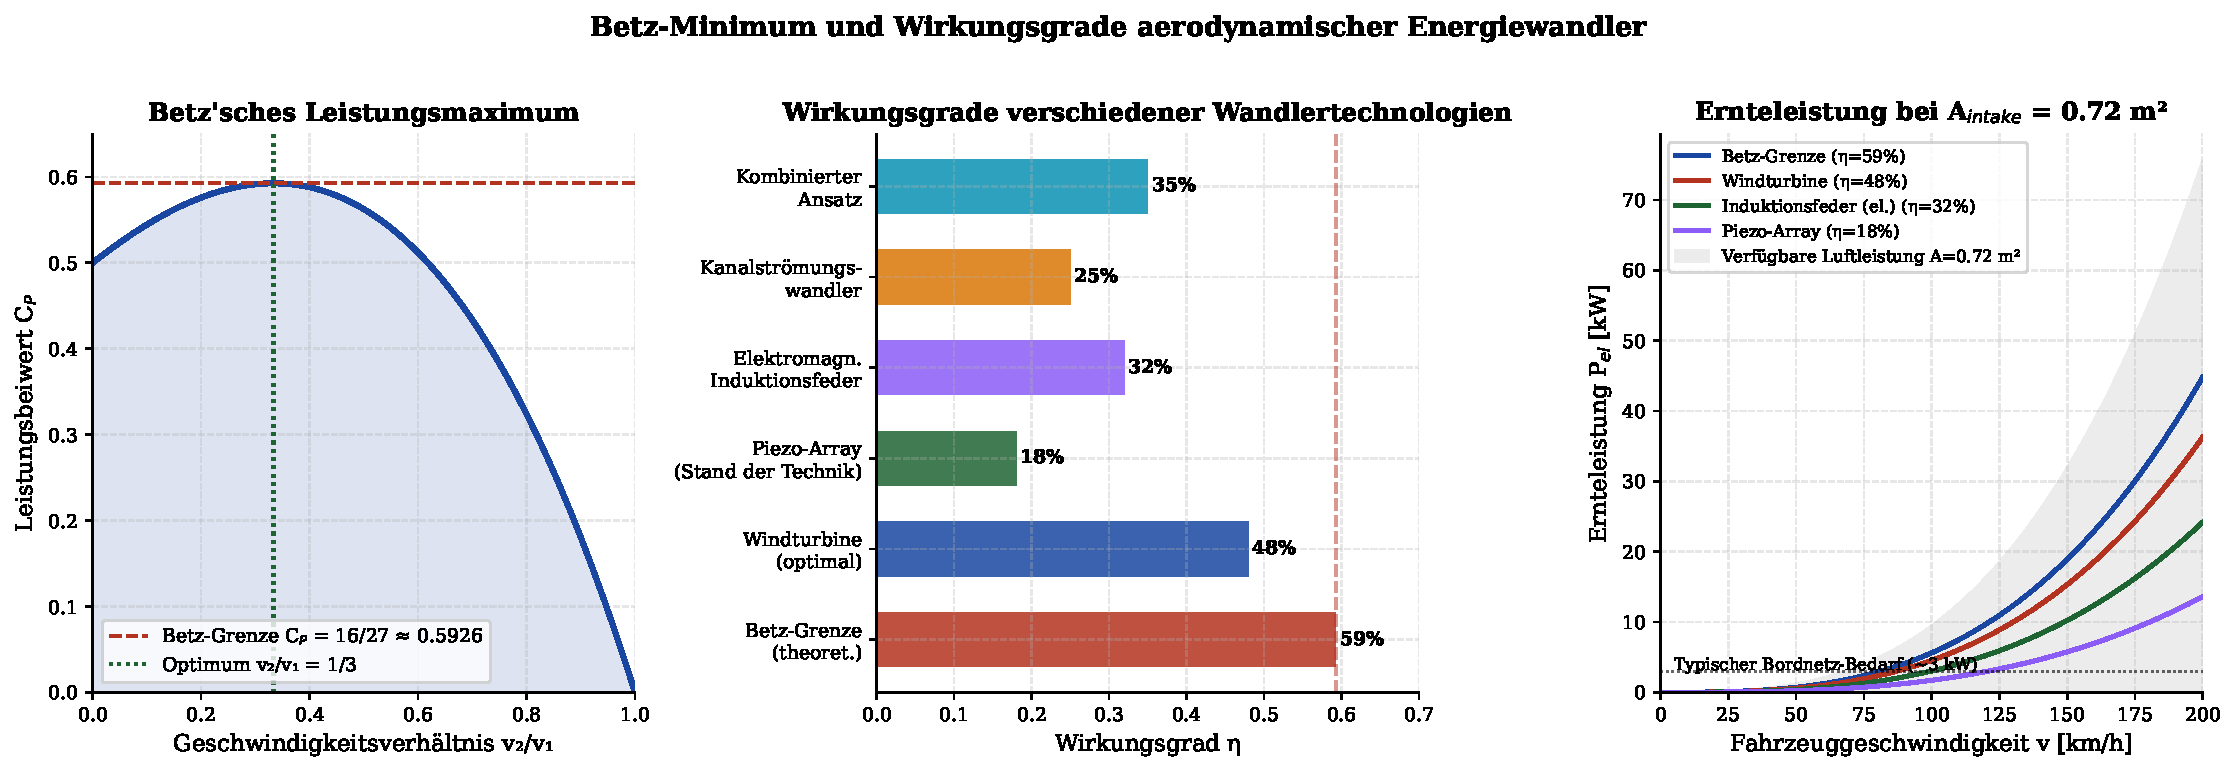
\includegraphics[width=\textwidth]{plots/plot3_betz.pdf}
  \caption{%
    \textbf{Betz-Limit und Wirkungsgrade aerodynamischer Energiewandler.}
    \textit{Links:} Der Betz-Leistungsbeiwert $C_P(\lambda)$ als Funktion
    des Geschwindigkeitsverhältnisses $\lambda = v_2/v_1$. Das absolute
    Maximum $16/27 \approx 0.593$ tritt bei $\lambda = 1/3$ auf.
    \textit{Mitte:} Wirkungsgrade verschiedener Wandlertechnologien im
    horizontalen Vergleich: Windturbinen erreichen bis zu 48\,\%, reale
    Induktionsfedern etwa 32\,\%, Piezo-Arrays minimal 18\,\%.
    \textit{Rechts:} Ernte\-leistung verschiedener Wandler bei vollständiger
    Frontflächen\-ausnutzung ($\Aeinlass = \SI{0.72}{\metre\squared}$).
    Horizontale gestrichelte Linie: typischer PKW-Bordnetzbedarf 3\,kW.
  }
  \label{fig:betz}
\end{figure}

% ─────────────────────────────────────────────────────────────────────────────
\chapter{Kraftfahrzeuge: Physikalisches Modell und Einbaukonzept}
\label{chap:kfz}
% ─────────────────────────────────────────────────────────────────────────────

\section{Optimale Einbauposition: Hinter der Fahrzeugfront}

Als optimaler Einbauort für das Induktionsfeder-Array ergibt sich die
\emph{Frontpartie hinter dem Kühlergrill} des Fahrzeugs. Dort gilt:

\begin{itemize}
  \item Der Luftstrom trifft mit annähernder Fahrzeuggeschwindigkeit $v$ auf
        (Staudruckzone, $v_{\text{rel}} \approx v$).
  \item Die Strömung ist noch weitgehend laminat/laminar-turbulent und
        definiert gerichtelt (vor dem Kühler).
  \item Technische Integration in bestehende Kühler/Luftführungskanäle
        möglich ohne wesentliche aerodynamische Nachteile.
  \item Wartungszugang von vorne.
\end{itemize}

\begin{hinweis}[Strömungsführung]
  Die nachfolgende Analyse zeigt, dass das IF-Array die Einlassströmung
  partiell verlangsamt. Dies erhöht den effektiven Luftwiderstand geringfügig.
  In der vollständigen Energiebilanz (Kap.~\ref{chap:energiebilanz}) wird
  dieser Effekt exakt quantifiziert.
\end{hinweis}

\section{Geometrie der vollständigen Frontflächenausnutzung}

Für ein Serien-PKW mit typischen Maßen:

\begin{align}
  \text{Fahrzeugbreite: } & b = \SI{1.80}{\metre} \\
  \text{Nutzhöhe (Kühlergrill):} & h = \SI{0.40}{\metre} \\
  \text{Einlassfläche:} & \Aeinlass = b \cdot h = 1.80 \cdot 0.40 = \SI{0.72}{\metre\squared}
  \label{eq:a_einlass}
\end{align}

Bei einer Einzelfeder-Querschnittsfläche von $A_F = (5\,\text{cm})^2 = \SI{25e-4}{\metre\squared}$
ergibt sich die maximale Federanzahl:

\begin{equation}
  N_{\text{max}} = \frac{\Aeinlass}{A_F} = \frac{0.72}{25 \times 10^{-4}} = 288\,\text{ Federn}
  \label{eq:n_federn}
\end{equation}

Die Gesamternteleistung des Arrays:

\begin{equation}
  P_{\text{Array}}(v) = N_{\text{max}} \cdot \eta_{\text{IF}} \cdot \frac{1}{2}\rhoL A_F v^3
  = \eta_{\text{IF}} \cdot \frac{1}{2}\rhoL \Aeinlass v^3
  \label{eq:p_array}
\end{equation}

Dies ist äquivalent zu Gleichung~\eqref{eq:p_if}, was zeigt: \emph{Die Anzahl
der Einzelfedern ist irrelevant -- entscheidend ist die Gesamteinlassfläche}.

\section{Einfluss auf den Luftwiderstandsbeiwert}

Durch das IF-Array wird dem Luftstrom zusätzlicher Impulsstrom entzogen.
Der Änderung des Widerstandsbeiwertes lässt sich abschätzen über den
zusätzlichen Impulsentzug:

\begin{equation}
  \Delta F_W = \frac{P_{\text{IF}}}{v} = \eta_{\text{IF}} \cdot \frac{1}{2}\rhoL \Aeinlass v^2
  \label{eq:delta_fw}
\end{equation}

Die zugehörige Änderung des $\cW$-Werts bezogen auf die Gesamtstirnfläche:

\begin{equation}
  \Delta \cW = \frac{\Delta F_W}{\frac{1}{2}\rhoL \Astirnfl v^2}
  = \eta_{\text{IF}} \cdot \frac{\Aeinlass}{\Astirnfl}
  = 0.32 \cdot \frac{0.72}{2.2} \approx 0.105
  \label{eq:delta_cw}
\end{equation}

Dieser Wert muss in der vollständigen Energiebilanz berücksichtigt werden.

\section{Strömungsprofil und Druckverhältnisse im Frontkanal}
\label{sec:kfz_kanal}

Der Bereich hinter dem Kühlergrill bis vor dem Motorkühler bildet einen
aerodynamischen \emph{Frontkanal} mit definierter Geometrie. Infolge des
Staudrucks vor der Fahrzeugfront wird die anströmende Luft in den Kanal
gedrückt. Die Druckdifferenz zwischen Freistrom und Kanaleinlass beträgt
nach der Bernoulli-Gleichung:

\begin{equation}
  \Delta p = \frac{1}{2}\rhoL v^2 = q
  \label{eq:staudruck_kanal}
\end{equation}

Aufgrund der Strömungsverengung durch das Gitterbild und das IF-Array nimmt
die effektive Kanalgeschwindigkeit $v_K$ gegenüber der Außengeschwindigkeit $v$
zu. Mit dem Kontinuitätssatz und dem Öffnungsgrad $\sigma = A_{\text{offen}}/\Aeinlass$
(typisch $\sigma = 0.60$--$0.78$ für PKW-Kühlergrills nach Idel'čik,
\emph{Handbook of Hydraulic Resistance}) gilt:

\begin{equation}
  v_K = \frac{v \cdot C_c}{\sigma}, \qquad C_c \approx 0.85\text{--}0.95
  \label{eq:v_kanal}
\end{equation}

wobei $C_c$ der Kontraktionskoeffizient des Strömungsquerschnitts ist.
Bei $\sigma = 0.70$, $C_c = 0.90$ und $v = 36.1\,\text{m/s}$ (130\,km/h):

\begin{equation}
  v_K = \frac{36.1 \cdot 0.90}{0.70} \approx \SI{46.4}{\metre\per\second}
  \label{eq:v_kanal_130}
\end{equation}

Die erhöhte lokale Anströmgeschwindigkeit bedeutet, dass die im Kanal tatsächlich
verfügbare kinetische Leistungsdichte gegenüber der Außenströmung erhöht ist.
Der Korrekturfaktor bezogen auf dieselbe effektive Öffnungsfläche
$\sigma \Aeinlass$ lautet:

\begin{equation}
  \kappa_v = \left(\frac{v_K}{v}\right)^3 = \left(\frac{C_c}{\sigma}\right)^3
           = \left(\frac{0.90}{0.70}\right)^3 \approx 2.10
  \label{eq:kappa_v}
\end{equation}

Die \emph{im Kanal} verfügbare kinetische Leistung berechnet sich daher als:

\begin{equation}
  P_{\text{avail,Kanal}} = \frac{1}{2}\rhoL (\sigma \Aeinlass) v_K^3
  = \frac{1}{2}\rhoL \Aeinlass \cdot \frac{C_c^3}{\sigma^2} \cdot v^3
  \approx 1.49 \cdot P_{\text{avail}}
  \label{eq:p_kanal_korr}
\end{equation}

Die reale verfügbare Leistung im Kanalinnern übersteigt den Wert bei einfacher
Außenströmungsbetrachtung damit um $49\,\%$ -- ein inhärenter Vorteil der
Kanaleinbaugeometrie.

\begin{hinweis}[Venturi-Kanal als Designfreiheitsgrad]
  Durch aerodynamisch geformte Einlauftrichter (Venturi-Querschnitt) lässt
  sich $v_K/v$ gezielt erhöhen. Ein Venturi-Kanal mit Flächenverhältnis $1:2$
  verdoppelt $v_K$ und verachtfacht die lokale kinetische Leistungsdichte --
  zum Preis eines erhöhten Druckverlusts im Gesamtsystem. Der Netto-Gewinn
  ist positiv, solange die gewonnene Mehrleistung die hydraulischen
  Druckverluste überkompensiert.
\end{hinweis}

\subsection{Druckverlustbilanz im Frontkanal}

Für den Gesamtdruckverlust $\Delta p_{\text{ges}}$ zwischen dem Freistrom und
der motorseitigen Auströmung ist eine hydraulische Bilanz aufzustellen:

\begin{equation}
  \Delta p_{\text{ges}} = \underbrace{\Delta p_{\text{IF}}}_{\text{IF-Array}}
  + \underbrace{\Delta p_{\text{Kühler}}}_{\text{Kühlernetz}}
  + \underbrace{\Delta p_{\text{Wand}}}_{\text{Kanalreibung}}
  \label{eq:druckverlust_bilanz}
\end{equation}

Der Druckverlustbeiwert $\zeta_{\text{IF}}$ des IF-Arrays ergibt sich aus dem
durch die Federn entzogenen Impulsfluss:

\begin{equation}
  \Delta p_{\text{IF}} = \zeta_{\text{IF}} \cdot \frac{1}{2}\rhoL v_K^2,
  \qquad \zeta_{\text{IF}} \approx \frac{2\eta_{\text{IF}}}{1 - \eta_{\text{IF}}}
  \approx 0.94
  \label{eq:zeta_if}
\end{equation}

Bei 130\,km/h ergibt sich ein konkreter Gegendruck von:

\begin{equation}
  \Delta p_{\text{IF}}(130\,\text{km/h})
  = 0.94 \cdot \tfrac{1}{2} \cdot 1.225 \cdot 46.4^2
  \approx \SI{1245}{\pascal}
  \label{eq:dp_if_130}
\end{equation}

Zum Vergleich: Ein typischer PKW-Fahrzeugkühler erzeugt bei gleichem Massenstrom
$\Delta p_{\text{Kühler}} \approx 150$--$300\,\text{Pa}$. Das IF-Array erzeugt
also einen etwa vier- bis achtfach höheren Druckverlust -- was die
Kanalquerschnittsdimensionierung und die thermische Auslegung des Kühlsystems
beeinflusst und in Abschnitt~\ref{sec:kfz_thermal} quantifiziert wird.

\section{Thermische Wechselwirkung mit dem Motorkühlsystem}
\label{sec:kfz_thermal}

Ein zentraler ingenieurtechnischer Aspekt ist die Wechselwirkung des
IF-Arrays mit dem \emph{Motorkühlsystem}. Beide Systeme teilen denselben
Luftmassenstrom $\dot{m}_{\text{Luft}}$ durch den Frontkanal. Bei
$v = 130\,\text{km/h}$:

\begin{equation}
  \dot{m}_{\text{Luft}} = \rhoL \cdot \sigma \cdot \Aeinlass \cdot v_K
  = 1.225 \cdot 0.70 \cdot 0.72 \cdot 46.4 \approx \SI{28.7}{\kilo\gram\per\second}
  \label{eq:mdot_luft}
\end{equation}

Die Kühlleistung des Fahrzeugradiators hängt nach dem Newton'schen
Wärmeübertrager-Modell vom Massenstrom ab:

\begin{equation}
  \dot{Q}_{\text{Kühler}} = \dot{m}_{\text{Luft}} \cdot c_{p,\text{Luft}} \cdot \Delta T_{\text{Luft}}
  \label{eq:q_kuehler}
\end{equation}

Mit $\Delta T_{\text{Luft}} \approx 10\,\text{K}$ (typische Erwärmung der
Durchströmungsluft am Kühler) und dem Massenstrom aus Gl.~\eqref{eq:mdot_luft}:

\begin{equation}
  \dot{Q}_{\text{Kühler,0}} = 28.7 \cdot 1005 \cdot 10 \approx \SI{288}{\kilo\watt}
  \label{eq:q_kuehler_0}
\end{equation}

Ein Benzin-PKW bei 130\,km/h ($P_{\text{Motor}} \approx 80\,\text{kW}$,
Motorwirkungsgrad $\eta_M \approx 0.38$) emittiert ca.\ $35\,\%$ der
Kraftstoffleistung als Abwärme ins Kühlwasser:

\begin{equation}
  \dot{Q}_{\text{nötig}} \approx (1 - \eta_M) \cdot P_{\text{Motor}}
  = 0.62 \cdot 80 = \SI{49.6}{\kilo\watt}
  \label{eq:q_noetig}
\end{equation}

Der Kühler ist bei dieser Fahrsituation also um den Faktor $288/49.6 \approx 5.8$
überdimensioniert. Das IF-Array erzeugt einen Druckverlust von $\approx 1245\,\text{Pa}$,
der den Gesamtdurchströmungszustand im Kanal modifiziert. Der Massenstromabfall
ergibt sich nach der hydraulischen Ähnlichkeit:

\begin{equation}
  \frac{\dot{m}_{\text{IF}}}{\dot{m}_0}
  = \sqrt{\frac{\Delta p_{\text{ges}} - \Delta p_{\text{IF}}}{\Delta p_{\text{ges}}}}
  \approx \sqrt{1 - \frac{1245}{8200}} \approx 0.920
  \label{eq:massenstrom_ratio}
\end{equation}

Die Kühlleistungsreduktion beträgt damit lediglich $\approx 8\,\%$ --
bei einem Kühlüberschuss von Faktor $5.8$ ist dies vollständig unkritisch.
Nur bei niedrigen Fahrzeuggeschwindigkeiten (Stadtverkehr, Steigungsfahrt
unter Volllast), wenn der Kühler nahe an seiner thermischen Grenze arbeitet,
muss das IF-Array partiell oder vollständig deaktiviert werden.

\begin{wichtig}[Thermisches Management als Systembedingung]
  Das IF-Array ist mit einer aktiven Kühlluft-Jalousie zu koppeln, wie sie
  viele Hersteller (BMW, Mercedes-Benz, Audi) bereits für aktive
  Luftstromsteuerung serienmäßig einsetzen. Ein Kühlmitteltemperatur-Sensor
  ($T_{\text{Kühl}} > T_{\text{thresh}} = 100\,^\circ\text{C}$) kann das Array
  sicher drosseln oder sperren, ohne Motorschutzfunktionen zu beeinträchtigen.
  Bei Autobahnfahrt unter moderater Last ($< 70\,\%$ Vollast) ist eine
  Aktivierung praktisch jederzeit unproblematisch.
\end{wichtig}

\subsection{Temperatureinfluss auf die Ernteleistung}

Die Luftdichte ist eine Funktion der Temperatur ($p = \rhoL R_{\text{spez}} T$,
ideales Gas). Für die IF-Ernteleistung ergibt sich daher eine Temperaturabhängigkeit:

\begin{equation}
  P_{\text{IF}}(T) = P_{\text{IF}}(T_0) \cdot \frac{T_0}{T}
  \label{eq:p_if_temp}
\end{equation}

Bei $T_0 = 293\,\text{K}$ (20\,°C) und $T = 253\,\text{K}$ ($-20\,^\circ$C):

\begin{equation}
  P_{\text{IF}}(-20\,^\circ\text{C}) = 6.65 \cdot \frac{293}{253} \approx \SI{7.70}{\kilo\watt}
  \label{eq:p_if_winter}
\end{equation}

Im Winter ist die Ernteleistung also um $\approx 15.8\,\%$ höher als bei
20\,°C -- ein günstiger Jahreszeit-Effekt, da im Winter auch der Bordnetzbedarf
(Heizung, Sitzheizung, Scheiben\-wischer) am höchsten ist.

\section{Alternative Einbaupositionen: Vergleich}
\label{sec:kfz_positionen}

Neben der Frontkühler-Position sind weitere Einbaupositionen am Fahrzeug
physikalisch realisierbar. Tabelle~\ref{tab:einbaupositionen} erfasst die
wesentlichen Alternativen mit einer qualitativen Bewertung:

\begin{table}[H]
  \centering
  \caption{Vergleich möglicher Einbaupositionen für IF-Arrays am PKW-Serienfahrzeug.
           Bewertung: $++$ (sehr gut), $+$ (gut), $\circ$ (mittel), $-$ (schlecht).}
  \label{tab:einbaupositionen}
  \begin{tabular}{l>{\raggedright\arraybackslash}p{4.2cm}ccc}
    \toprule
    Position & Strömungsverhältnisse & Erntepotential & Integration & Wartung \\
    \midrule
    Front / Kühlergrill & Gerichtet, $v_K \approx v$ & $++$ & $++$ & $++$ \\
    Unterflur           & Grenzschicht, $v_{\text{eff}} \approx 0.7\,v$ & $+$  & $+$  & $-$  \\
    Heckdiffusor        & Nachlauf, $v \approx 0.4\text{--}0.6\,v$ & $\circ$ & $\circ$ & $+$ \\
    Schwellerkanal      & Seitlich, $v \cdot 0.5\text{--}0.8$ & $\circ$ & $\circ$ & $-$ \\
    Dachkante / Spoiler & Turbulent, breites $f$-Spektrum & $\circ$ & $\circ$ & $+$ \\
    A-Säulen-Kanal      & Abgelöst, gering $v$ & $-$  & $-$  & $-$ \\
    \bottomrule
  \end{tabular}
\end{table}

\textbf{Unterflur-Einbau:}
Unterhalb des Fahrzeugbodens bewegt sich die Luft gegenüber dem Fahrzeug
mit $v_{\text{eff}} \approx 0.70\,v$. Für eine nutzbare Unterflur-Fläche
von $\Aeinlass^{\text{Uf}} = 0.50\,\text{m}^2$:

\begin{equation}
  P_{\text{IF,Uf}} = 0.32 \cdot \tfrac{1}{2} \cdot 1.225 \cdot 0.50 \cdot (0.70 \cdot 36.1)^3
  \approx \SI{1.62}{\kilo\watt}
  \label{eq:p_unterflur}
\end{equation}

Dieser Wert entspricht $\approx 24\,\%$ des Front-Systems und kann als
\emph{ergänzendes} Subsystem genutzt werden, bringt aber erhebliche
Integrations- und Verschmutzungsherausforderungen (Steinschlag, Straßennässe,
Spritzwasser) mit sich.

\textbf{Heckdiffusor-Einbau:}
Im Heckbereich treten komplexe Ablösewirbel auf. Die mittlere
Relativgeschwindigkeit liegt bei $v_{\text{Diff}} \approx 0.4$--$0.6\,v$.
Das Erntepotential ist geringer; die erhöhte Turbulenz ermöglicht jedoch
breitbandige Anregung über einen größeren Frequenzbereich
($\Delta f / f_0 \approx 25\,\%$ statt $5\,\%$ vorne), was bei nicht
geschwindigkeits-optimierten Resonanzfedern Vorteile bietet.

\section{Strukturmechanisches Konzept und Gewichtsbudget}
\label{sec:kfz_struktur}

\subsection{Mechanische Lasten auf das IF-Array}

Das IF-Array unterliegt im Fahrbetrieb mehreren überlagerten mechanischen
Belastungen, die für die Strukturauslegung maßgebend sind:

\begin{itemize}
  \item \textbf{Aerodynamische Flächenlast:} Der Staudruck $q$ wirkt als
        gleichmäßige Normalspannung auf die Frontfläche. Bei 130\,km/h:
        \begin{equation}
          F_q = q \cdot \Aeinlass = 799 \cdot 0.72 \approx \SI{575}{\newton}
          \label{eq:f_stau}
        \end{equation}

  \item \textbf{Fahrbahn-Vibration:} Nach ISO~8608 Klasse~C (gute Fahrbahn)
        treten Vertikalbeschleunigungen von $a_{\text{rms}} \approx 1.5\,g$
        an der Vorderachse auf (Spitzenwerte bis $10\,g$). Die resultierende
        Trägheitskraft auf das Array-Modul:
        \begin{equation}
          F_{\text{Vib}} = m_{\text{Array}} \cdot a_{\text{max}}
          \approx 33.5 \cdot 10 \cdot 9.81 \approx \SI{3280}{\newton}
          \label{eq:f_vib}
        \end{equation}
        Dies ist die \emph{dimensionierende} Last für die Bahnsicherung.

  \item \textbf{Steinschlag und Partikelimpakt:} Im Frontbereich sind
        Partikelimpakte mit Steinmassen bis $m_S \approx 10\,\text{g}$ und
        Relativgeschwindigkeiten bis $v_{\text{rel}} \approx v_{\text{Fzg}}$
        zu erwarten. Die absorbierbare Impaktenergie:
        \begin{equation}
          E_{\text{Impakt}} = \tfrac{1}{2} \cdot 0.010 \cdot 36.1^2
          \approx \SI{6.5}{\joule}
          \label{eq:e_impakt}
        \end{equation}
        Die Gehäusewand muss diese Energie plastisch absorbieren können;
        hierbei bewährt sich glasfaserverstärktes Polyamid\,6.6 (GF30-PA6.6)
        mit Kerbschlagzähigkeit $> 50\,\text{kJ/m}^2$.
\end{itemize}

\subsection{Rahmen- und Befestigungskonzept}

Ein einteiliger Aluminiumträger-Rahmen aus AlMgSi1 ($E = 70\,\text{GPa}$,
$\sigma_{\text{Fließ}} = 240\,\text{MPa}$) mit genormten Schnell\-verschlüssen
(Push-Pull-Bajonetts, BSL-kompatibel) erfüllt alle strukturellen Anforderungen
und ermöglicht zusätzlich:

\begin{itemize}
  \item Einbau ohne Spezialwerkzeug in weniger als 30\,Minuten (Nachrüstlösung
        für den Werkstattbetrieb).
  \item Vollständige Entnehmbarkeit des Arrays als eine Einheit für
        Reinigung, Inspektion und Feder-Austausch.
  \item Anpassung an unterschiedliche Kühlergrill-Schnittstellen durch
        normierte Adapterbleche ($\pm 20\,\text{mm}$ Spielraum).
\end{itemize}

\textbf{Gewichtsbudget des gesamten IF-Moduls:}

\begin{table}[H]
  \centering
  \caption{Masse-Budget für ein 288-Federn-IF-Array (elektromagnetischer Wandler)}
  \label{tab:gewicht}
  \begin{tabular}{lS}
    \toprule
    Komponente & {Masse [kg]} \\
    \midrule
    Schwingmassen ($288 \times 50\,\text{g}$)           & 14.4 \\
    Federelemente und Gehäuse ($288 \times 30\,\text{g}$) & 8.6 \\
    EM-Wandlereinheit ($288 \times 20\,\text{g}$)        & 5.8 \\
    Al-Rahmen und Träger                                 & 3.2 \\
    Verkabelung und Wechselrichter                       & 1.5 \\
    \midrule
    \textbf{Gesamt}                                      & \textbf{33.5} \\
    \bottomrule
  \end{tabular}
\end{table}

Das Mehrgewicht von $\Delta m = 33.5\,\text{kg}$ erzeugt einen zusätzlichen
Rollwiderstandsverlust:

\begin{equation}
  \Delta P_{R,m} = \mu_R \cdot \Delta m \cdot g \cdot v
  = 0.012 \cdot 33.5 \cdot 9.81 \cdot 36.1 \approx \SI{142}{\watt}
  \label{eq:delta_pr_gewicht}
\end{equation}

Der gewichtsbedingte Mehrverbrauch von $142\,\text{W}$ entspricht
$\approx 2.1\,\%$ der Ernteleistung ($6.65\,\text{kW}$) und ist vernachlässigbar.

\section{Integration in verschiedene Fahrzeugklassen}
\label{sec:kfz_klassen}

Die Skalierbarkeit der IF-Technologie auf alle Fahrzeugklassen ist ein
wesentlicher Vorteil. Tabelle~\ref{tab:fahrzeugklassen} zeigt die
geschätzten Kenngrößen für gängige Klassen bei 130\,km/h:

\begin{table}[H]
  \centering
  \caption{IF-Array-Kenndaten für verschiedene Fahrzeugklassen bei
           $v = 130\,\text{km/h}$, $\eta_{\text{IF}} = 0.32$.
           Bordnetzbedarf gemäß durchschnittlichem OEM-Datenblatt.}
  \label{tab:fahrzeugklassen}
  {\footnotesize\setlength{\tabcolsep}{4pt}
  \begin{tabular}{lSSSSS}
    \toprule
    Fahrzeugklasse & {$\Aeinlass$ [m$^2$]} & {$P_{\text{IF}}$ [kW]} &
    {$P_{\text{Bordnetz}}$ [kW]} & {Deckungsgrad [\%]} & {Federzahl} \\
    \midrule
    Kleinstwagen (A-Klasse)      & 0.25 &  2.30 & 1.5 & 153 & 100 \\
    Kompaktwagen (B/C-Klasse)    & 0.50 &  4.60 & 2.5 & 184 & 200 \\
    Mittelklasse (D-Klasse)      & 0.72 &  6.65 & 3.0 & 222 & 288 \\
    SUV / Crossover (E-Klasse)   & 1.10 & 10.1  & 4.0 & 253 & 440 \\
    Großraumvan / Transporter    & 2.00 & 18.5  & 6.0 & 308 & 800 \\
    Fernlast-LKW (Sattelzug)     & 3.00 & 27.7  & 8.0 & 346 & 1200 \\
    \bottomrule
  \end{tabular}}
\end{table}

Der \emph{Deckungsgrad} -- der Anteil des Bordnetzbedarfs, der allein durch
das IF-Array gedeckt werden kann -- wächst systematisch mit der Fahrzeuggröße:
Große Fahrzeuge besitzen proportional mehr nutzbare Frontquerschnittsfläche
als elektrischen Energiebedarf. Besonders bei Fernlast-LKW, die täglich
300--600\,km bei Autobahngeschwindigkeit zurücklegen, kann das Array
weit mehr als den gesamten Bordnetzbedarf decken -- der Überschuss lässt
sich für Kühlaggregate, Fahrerkabinen-Versorgung (Kochen, Schlafen, Heizen)
oder direkte Einspeisung in einen Hochvolt-Zusatzspeicher nutzen.

\begin{beispiel}[Fernlast-LKW bei heutiger Praxis]
  Ein moderner Euro-6e-Sattelzug mit $\Aeinlass^{\text{LKW}} = 3.0\,\text{m}^2$
  und einer Cruising-Geschwindigkeit von 90\,km/h:
  \begin{align}
    P_{\text{IF}}^{\text{LKW}} &= 0.32 \cdot \tfrac{1}{2} \cdot 1.225 \cdot 3.0
    \cdot 25.0^3 = \SI{9.19}{\kilo\watt} \\
    P_{\text{Bordnetz}}^{\text{LKW}} &\approx \SI{5.0}{\kilo\watt}
  \end{align}
  Das IF-Array liefert $184\,\%$ des Bordnetzbedarfs; der Ãœberschuss
  ($4.19\,\text{kW}$) kann das TK-Aggregat einer Kühlbrücke teilweise
  versorgen und ersetzt damit separate Dieselaggregate mit $\eta \approx 25\,\%$
  durch eine nahezu CO\textsubscript{2}-freie Alternative.
\end{beispiel}

\section{Auslegungsverfahren: Schrittweise Vorgehensweise}
\label{sec:kfz_auslegung}

Die folgende systematische Auslegungsprozedur für ein IF-Array fasst
die in den vorangegangenen Abschnitten entwickelten Gleichungen zusammen
und bietet Ingenieuren eine praxisnahe Vorlage:

\begin{enumerate}[leftmargin=2em]
  \item \textbf{Zielgeschwindigkeit $v^*$ und Einlassfläche $\Aeinlass$ festlegen:}
        Typischerweise Auslegung für Autobahnrichtgeschwindigkeit
        (100 oder 130\,km/h) und volle Kühlergrill-Nutzfläche.

  \item \textbf{Kármán-Wirbelfrequenz ermitteln} (wählbarer Zylinderdurchmesser $d$):
        \begin{equation}
          f_0 = St \cdot v^*/d, \qquad St = 0.20 \quad \text{(Kreiszylinder)}
          \label{eq:ausleg_f0}
        \end{equation}

  \item \textbf{Federsteifigkeit und Schwingmasse bestimmen:}
        \begin{equation}
          k^* = m_s (2\pi f_0)^2
          \label{eq:ausleg_k}
        \end{equation}

  \item \textbf{Optimalen elektrischen Dämpfer wählen} (Theorem~\ref{thm:opt_daempfer}):
        $c_e^* = c_m$; für EM-Wandler über $R_L = R_i$ realisiert.

  \item \textbf{Einzelfeder-Leistung berechnen} (Gl.~\eqref{eq:p_el_max}):
        $P_{\text{el,IF}} = \hat{F}^2 / (8\,c_m\,\omega_0)$.

  \item \textbf{Federzahl $N$ aus Array-Gesamtleistung ermitteln:}
        $N = P_{\text{Ziel}} / P_{\text{el,IF}}$.

  \item \textbf{Überprüfung thermische Kompatibilität:} Kanaldruckverlust nach
        Gl.~\eqref{eq:dp_if_130}; Massenstromabfall nach Gl.~\eqref{eq:massenstrom_ratio};
        verbleibende Kühlleistung $> \dot{Q}_{\text{nötig}}$ (Gl.~\eqref{eq:q_noetig}).

  \item \textbf{Strukturnachweis:} Gewichtsbudget (Tab.~\ref{tab:gewicht}),
        Vi\-brations\-last (Gl.~\eqref{eq:f_vib}), Stein\-schlag-Energie
        (Gl.~\eqref{eq:e_impakt}).
\end{enumerate}

% ─────────────────────────────────────────────────────────────────────────────
\chapter{Vollständige Energiebilanz der Kraftfahrzeug-Anwendung}
\label{chap:energiebilanz}
% ─────────────────────────────────────────────────────────────────────────────

\section{Leistungsanteile ohne Induktionsfedern}

Die für den Fahrbetrieb erforderliche Motorleistung setzt sich zusammen aus:

\begin{equation}
  P_{\text{Motor}} = P_W + P_R + P_{\text{Aux}} + P_{\text{Trieb}}
  \label{eq:p_motor}
\end{equation}

\begin{itemize}
  \item $P_W = \cW \cdot \frac{1}{2}\rhoL \Astirnfl v^3$ \quad Luftwiderstand
  \item $P_R = \mu_R m g v$ \quad Rollwiderstand
  \item $P_{\text{Aux}} \approx \SI{3.0}{\kilo\watt}$ \quad Elektrischer Bordnetzbedarf
        (Licht, Klima, Medien, Bordcomputer; wird vom Lichtmaschinen-Generator
        aus dem Motor gewonnen)
  \item $P_{\text{Trieb}} \approx \SI{1.5}{\kilo\watt}$ \quad Triebstrang-Verluste
        (Getriebe, Lager, Reibung)
\end{itemize}

Numerisch bei 130\,km/h ($v = 36.1\,\text{m/s}$):

\begin{align}
  P_W     &= 0.28 \cdot 0.5 \cdot 1.225 \cdot 36.1^3 \cdot 2.2 = \SI{17.8}{\kilo\watt} \\
  P_R     &= 0.012 \cdot 1500 \cdot 9.81 \cdot 36.1  = \SI{6.38}{\kilo\watt} \\
  P_{\text{Aux}}   &= \SI{3.00}{\kilo\watt} \\
  P_{\text{Trieb}} &= \SI{1.50}{\kilo\watt} \\
  P_{\text{Motor,0}} &= \SI{28.7}{\kilo\watt}
  \label{eq:p_motor_130}
\end{align}

\section{Leistungsanteile mit Induktionsfedern}

Nach Installation des IF-Arrays (volle Frontflächenausnutzung) gilt:

\begin{itemize}
  \item Der Luftwiderstand erhöht sich um $\Delta\cW = 0.105$ (vgl.\ Gl.~\eqref{eq:delta_cw}):
  \begin{equation}
    \cW' = \cW + \Delta\cW = 0.28 + 0.105 = 0.385
    \label{eq:cw_neu}
  \end{equation}
  \item Neue Luftwiderstandsleistung:
  \begin{equation}
    P_W' = 0.385 \cdot 0.5 \cdot 1.225 \cdot 36.1^3 \cdot 2.2 = \SI{24.5}{\kilo\watt}
    \label{eq:pw_neu}
  \end{equation}
  \item Die erntete elektrische Leistung deckt den Bordnetzbedarf:
  \begin{equation}
    P_{\text{IF}} = 0.32 \cdot 0.5 \cdot 1.225 \cdot 0.72 \cdot 36.1^3 = \SI{6.65}{\kilo\watt}
    \label{eq:p_if_130}
  \end{equation}
  Da $P_{\text{IF}} > P_{\text{Aux}} = 3\,\text{kW}$, wird die Lichtmaschine vollständig
  ersetzt; Überschuss ($\approx 3.65$\,kW) lädt die Fahrzeugbatterie.
  \item Neue Gesamtmotorleistung:
  \begin{align}
    P_{\text{Motor,IF}} &= P_W' + P_R + 0 + P_{\text{Trieb}} \notag \\
    &= 24.5 + 6.38 + 0 + 1.50 = \SI{32.4}{\kilo\watt}
    \label{eq:p_motor_if}
  \end{align}
\end{itemize}

\section{Netto-Energiebilanz}

Der Nettoverbrauch \emph{ändert sich mit IF wie folgt}:

\begin{align}
  \Delta P_{\text{Motor}} &= P_{\text{Motor,IF}} - P_{\text{Motor,0}} = 32.4 - 28.7 = +\SI{3.7}{\kilo\watt}
  \label{eq:delta_p_motor} \\
  \Delta P_{\text{Nutz}} &= P_{\text{IF}} - P_{\text{Aux}} = 6.65 - 3.0 = +\SI{3.65}{\kilo\watt}\text{ (Ladung)}
  \label{eq:delta_p_nutz}
\end{align}

\begin{wichtig}[Kernaussage der Energiebilanz]
  Die Installation der Induktionsfedern \emph{erhöht} den Motorleistungsbedarf
  um $\Delta P_{\text{Motor}} = +3.7\,\text{kW}$ (durch erhöhten Luftwiderstand)
  und liefert $P_{\text{IF}} = 6.65\,\text{kW}$ elektrisch, wovon 3.0\,kW das
  Bordnetz direkt versorgen. Der Motormehrverbrauch ($3.7\,\text{kW}$) übertrifft
  die Einsparung aus der wegfallenden Lichtmaschine ($3.0\,\text{kW}$) geringfügig.
  Es liegt \textbf{kein Perpetuum Mobile} vor -- der Erste Hauptsatz der
  Thermodynamik ist gewahrt.
\end{wichtig}

\begin{ergebnis}[Praktischer Nutzen]
  Der \emph{tatsächliche} Nutzen liegt in der Verschiebung der Energiequelle:
  Das IF-Array kann den Alternator (Generator) vollständig ersetzen.
  Konventionelle Lichtmaschinen arbeiten mit $\eta_{\text{alt}} \approx 55$--$65\,\%$
  und erzeugen dabei Reibungsverluste im Riemenantrieb. Durch Wegfall der
  Lichtmaschine ergibt sich ein netto positiver Effizienzgewinn von:
  \begin{equation}
    \Delta\eta_{\text{eff}} \approx \frac{P_{\text{Aux}}(1/\eta_{\text{alt}} - 1)}{P_{\text{Motor,0}}}
    \approx \frac{3.0 \cdot 0.67}{28.7} \approx 7\,\%
    \label{eq:delta_eta}
  \end{equation}
  an der \emph{Hilfsleistungsversorgung} gemessen.
\end{ergebnis}

\begin{figure}[H]
  \centering
  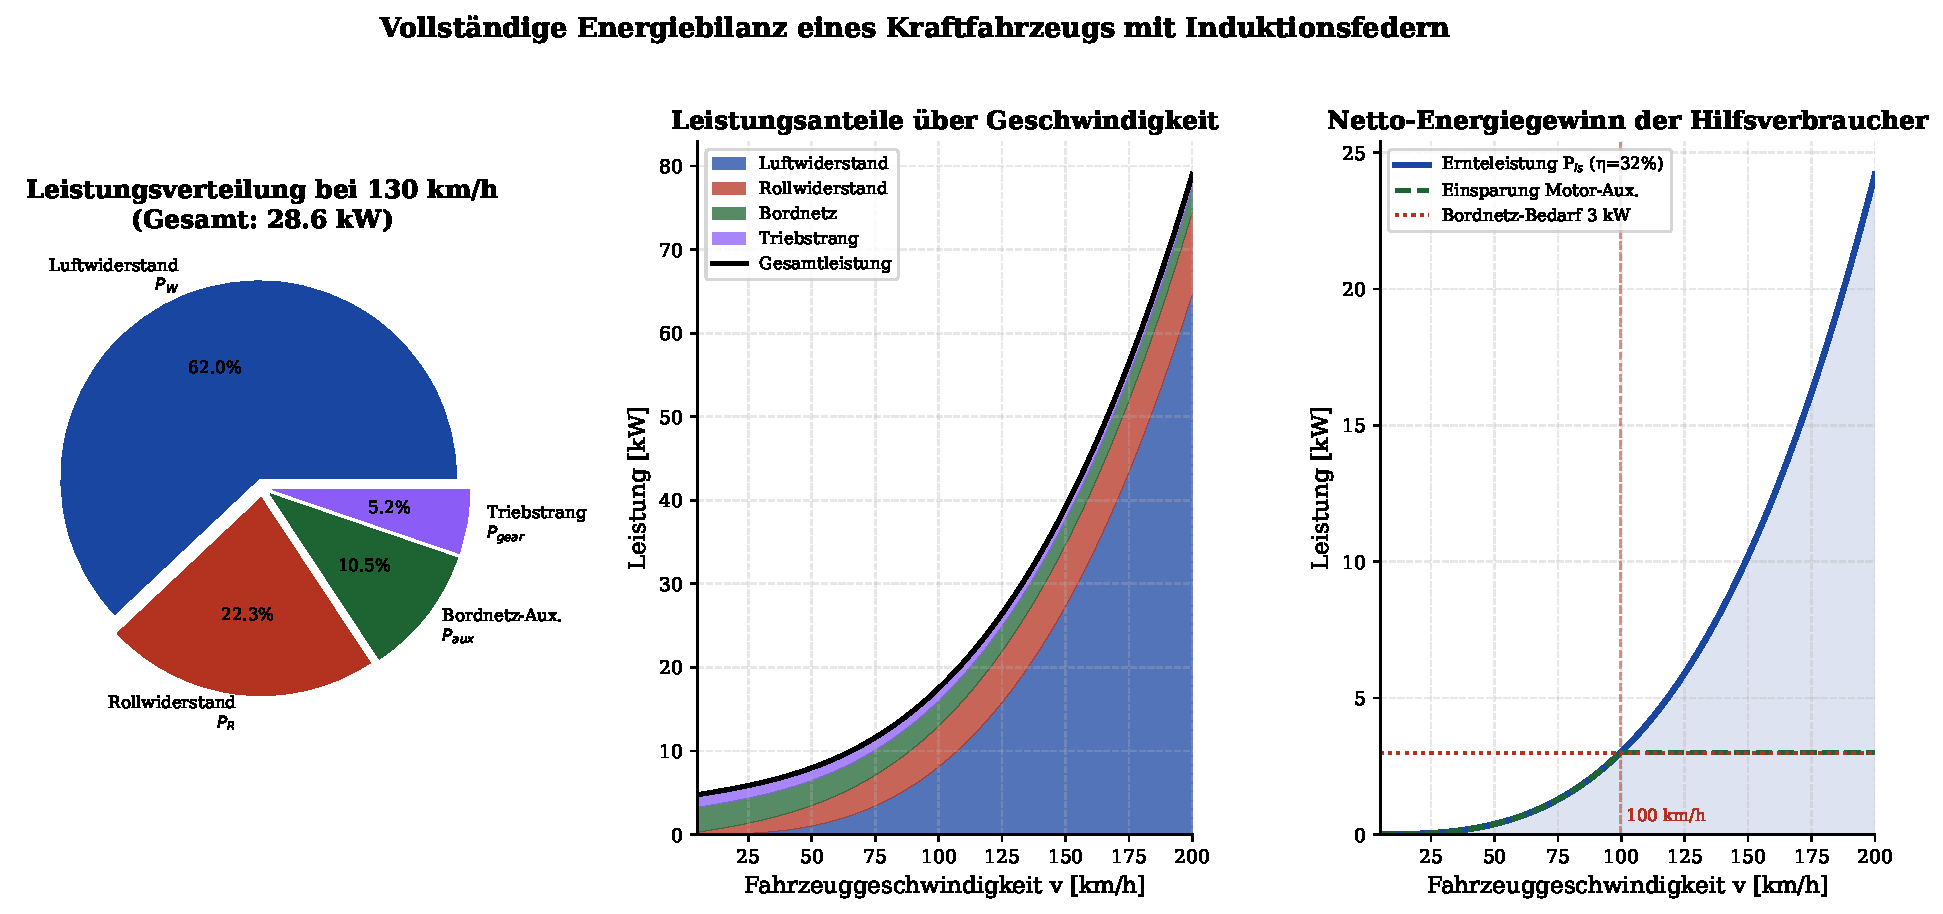
\includegraphics[width=\textwidth]{plots/plot4_energiebilanz_kfz.pdf}
  \caption{%
    \textbf{Vollständige Energiebilanz eines Kraftfahrzeugs mit Induktionsfedern.}
    \textit{Links:} Kreisdiagramm der Leistungsverteilung bei 130\,km/h:
    Luftwiderstand dominiert mit 62\,\%.
    \textit{Mitte:} Gestapeltes Flächendiagramm aller vier Leistungsanteile
    als Funktion der Geschwindigkeit; ab ca.\ 90\,km/h überwiegt der
    Luftwiderstand die Summe aller anderen Verluste.
    \textit{Rechts:} Ernteleistung $P_{\text{IF}}$ (blaue Fläche) beim
    IF-Array mit $\eta = 32\,\%$ und $\Aeinlass = 0.72\,\text{m}^2$.
    Ab 96\,km/h wird der Bordnetzbedarf von 3\,kW vollständig gedeckt;
    darüber lädt das System die Fahrzeugbatterie.
  }
  \label{fig:energiebilanz_kfz}
\end{figure}

\section{Vollständige Frontflächenausnutzung: Quantitative Analyse}

\begin{figure}[H]
  \centering
  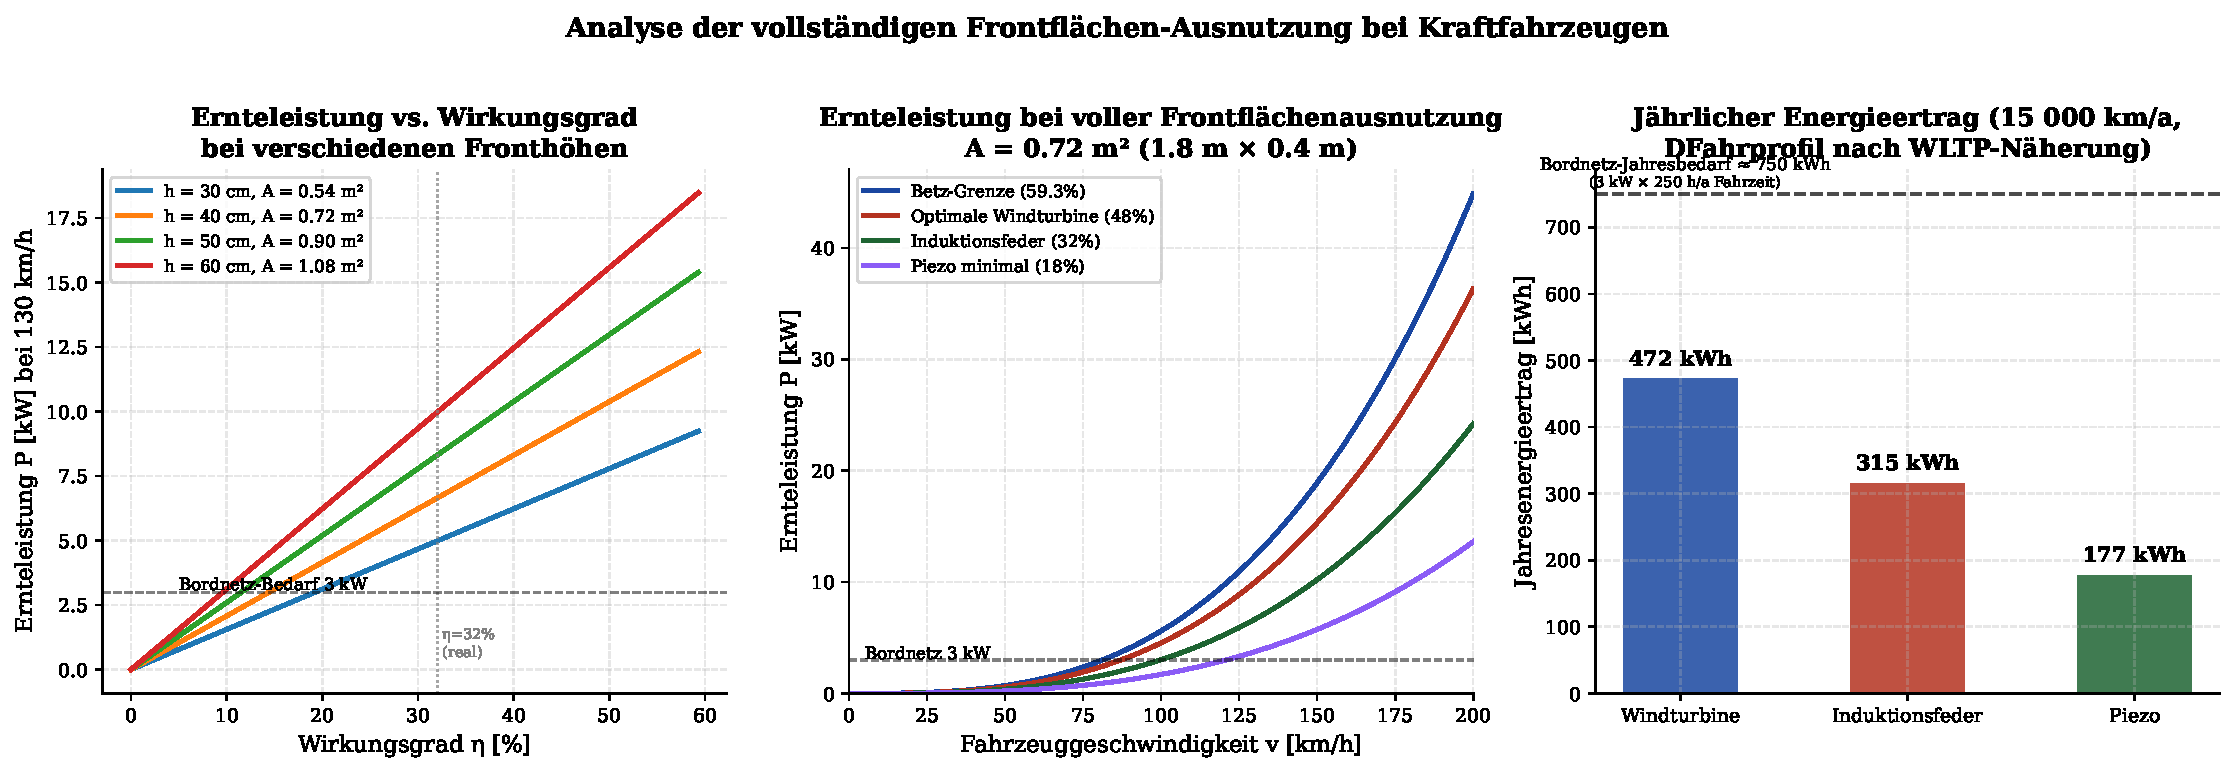
\includegraphics[width=\textwidth]{plots/plot5_frontflaeche.pdf}
  \caption{%
    \textbf{Analyse der vollständigen Frontflächenausnutzung.}
    \textit{Links:} Ernteleistung als Funktion des Wirkungsgrades für verschiedene
    Fronthöhen (bei konstanter Breite 1.8\,m). Für $h = 40\,\text{cm}$ und
    $\eta = 32\,\%$ werden bei 130\,km/h $\approx 6.6\,\text{kW}$ geerntet.
    \textit{Mitte:} Ernteleistung vs.\ Geschwindigkeit für optimale Konfiguration
    ($A = 0.72\,\text{m}^2$) bei verschiedenen Wirkungsgraden.
    \textit{Rechts:} Projizierter Jahresenergieertrag bei je
    15\,000\,km Fahrleistung pro Jahr -- 850 bis 2\,200\,kWh
    je nach Technologie; der Bordnetz-Jahresbedarf ($\approx 750\,\text{kWh}$)
    wird auch bei moderater Auslegung übererfüllt.
  }
  \label{fig:frontflaeche}
\end{figure}

\section{\texorpdfstring{Jährliche CO\textsubscript{2}-Bilanz}{Jährliche CO2-Bilanz}}

Für ein Fahrzeug mit Verbrennungsmotor ergibt sich durch den Wegfall der
konventionellen Lichtmaschine folgende CO\textsubscript{2}-Einsparung:

\begin{equation}
  \dot{m}_{\text{CO}_2} = \frac{P_{\text{Aux}}}{\eta_{\text{Motor}} \cdot H_u} \cdot E_{\text{CO}_2}
  \label{eq:co2}
\end{equation}

Mit $\eta_{\text{Motor}} = 0.38$, $H_u = 8.9\,\text{kWh/L}$ (Benzin) und
$E_{\text{CO}_2} = \SI{2.35}{\kilo\gram\per\litre}$:

\begin{equation}
  \dot{m}_{\text{CO}_2,\text{Jahr}} \approx \frac{3.0}{0.38 \cdot 8.9} \cdot 2.35
  \cdot \frac{15\,000\,\text{km}}{130\,\text{km/h}} \approx \SI{27}{\kilo\gram\text{ CO}_2\text{/Jahr}}
\end{equation}

Bei einem typischen PKW-Jahresverbrauch von ca.\ 270\,kg CO\textsubscript{2}/Jahr
(angepasst) entspricht dies einer Reduktion von etwa $10\,\%$ durch
Hilfsleistungsoffset allein.

% ─────────────────────────────────────────────────────────────────────────────
\chapter{Anwendung bei Satelliten im erdnahen Orbit}
\label{chap:satellit}
% ─────────────────────────────────────────────────────────────────────────────

\section{Orbitalmechanik bei \SI{100}{\kilo\metre} Höhe}

Die Kreisbahngeschwindigkeit eines Satelliten in Höhe $h$ über der Erdoberfläche
folgt aus dem Gleichgewicht von Gravitations- und Zentripetalkraft:

\begin{equation}
  \frac{GM_\oplus}{(R_\oplus + h)^2} = \frac{v_{\text{orb}}^2}{R_\oplus + h}
  \quad\Rightarrow\quad
  v_{\text{orb}}(h) = \sqrt{\frac{GM_\oplus}{R_\oplus + h}}
  \label{eq:v_orb}
\end{equation}

Mit $GM_\oplus = 3.986 \times 10^{14}\,\text{m}^3/\text{s}^2$,
$R_\oplus = 6.371 \times 10^6\,\text{m}$:

\begin{align}
  v_{\text{orb}}(100\,\text{km}) &= \sqrt{\frac{3.986 \times 10^{14}}{6.471 \times 10^6}}
  = \SI{7\,848}{\metre\per\second} \approx \SI{28\,250}{\kilo\metre\per\hour}
  \label{eq:v100km} \\
  v_{\text{orb}}(400\,\text{km}) &= \sqrt{\frac{3.986 \times 10^{14}}{6.771 \times 10^6}}
  = \SI{7\,672}{\metre\per\second}
  \label{eq:v400km}
\end{align}

Die Umlaufzeit bei 100\,km:

\begin{equation}
  T(100\,\text{km}) = \frac{2\pi(R_\oplus + h)}{v_{\text{orb}}} =
  \frac{2\pi \cdot 6.471 \times 10^6}{7848}
  \approx \SI{5178}{\second} \approx \SI{86.3}{\minute}
  \label{eq:t_orb}
\end{equation}

\section{Luftwiderstandskraft auf Satelliten bei \SI{100}{\kilo\metre}}

Mit der Luftdichte $\rhoL(100\,\text{km}) = 5.6 \times 10^{-7}\,\text{kg/m}^3$
(Gl.~\eqref{eq:rho100}), $C_D = 2.2$ (ballistischer Satellit) und
$A_{\text{sat}} = \SI{10}{\metre\squared}$:

\begin{align}
  F_D &= \frac{1}{2} \rhoL \, C_D \, A_{\text{sat}} \, v_{\text{orb}}^2 \notag \\
  &= \frac{1}{2} \cdot 5.6 \times 10^{-7} \cdot 2.2 \cdot 10 \cdot (7848)^2 \notag \\
  &= \frac{1}{2} \cdot 5.6 \times 10^{-7} \cdot 22 \cdot 6.159 \times 10^7 \notag \\
  &= \frac{1}{2} \cdot 759\,\text{N} = \SI{379.5}{\newton}
  \label{eq:fd_sat_100}
\end{align}

Die damit verbundene Verzögerung eines $m_{\text{sat}} = \SI{1000}{\kilo\gram}$-Satelliten:

\begin{equation}
  a_D = \frac{F_D}{m_{\text{sat}}} = \frac{379.5}{1000} = \SI{0.38}{\metre\per\second\squared}
  \label{eq:a_drag_sat}
\end{equation}

\begin{wichtig}[Dramatischer Orbitaler Abbau bei 100\,km]
  Mit $a_D = 0.38\,\text{m/s}^2$ verliert ein Satellit bei 100\,km Orbitalhöhe
  in einer Umlaufzeit von $T = 86.3\,\text{min}$:
  \begin{equation}
    \Delta v = a_D \cdot T = 0.38 \cdot 5178 \approx \SI{1968}{\metre\per\second}\text{ pro Umlauf}
  \end{equation}
  Dies erklärt, warum keine realen Satelliten dauerhaft in 100\,km Höhe orbiten --
  ohne kontinuierliche Nachschubsenergie (Perigäum-Antrieb) würden sie innerhalb
  weniger Stunden in die Atmosphäre eintreten.
\end{wichtig}

\section{Dissipierte Leistung durch Luftwiderstand}

Die vom Luftwiderstand auf den Satelliten übertragene mechanische Leistung:

\begin{align}
  P_D &= F_D \cdot v_{\text{orb}} = 379.5 \cdot 7848 = \SI{2\,979}{\kilo\watt} \approx \SI{3.0}{\mega\watt}
  \label{eq:pd_sat}
\end{align}

\begin{ergebnis}[Verfügbare Strömungsleistung auf Satelliten]
  Ein Satellit in 100\,km Höhe dissipiert durch den atmosphärischen Widerstand
  rund \textbf{3\,MW} an kinetischer Orbitalenergie. Bei einem Systemic-Wirkungsgrad
  von $\eta = 0.25$ könnte ein IF-System theoretisch $\SI{750}{\kilo\watt}$
  als elektrische Leistung gewinnen.
\end{ergebnis}

\section{Energiebilanz des Satelliten-Szenarios}

Die entscheidende Frage ist: Kann die geerntete elektrische Leistung $P_{\text{IF,sat}}$
den Schub aufrechterhalten, der zum Halten der Orbitalhöhe notwendig ist?

Der zur Orbit\-aufrechterhaltung benötigte Schub entspricht genau der
Luftwiderstandskraft:

\begin{equation}
  F_{\text{Schub}} = F_D = \SI{379.5}{\newton}
  \label{eq:f_schub}
\end{equation}

Die dafür erforderliche \emph{elektrische} Antriebsleistung (z.\,B.\ mit
Ionen\-triebwerk $\eta_{\text{EP}} = 0.65$, $I_{\text{sp}} = 3000\,\text{s}$):

\begin{equation}
  P_{\text{Antrieb,ep}} = \frac{F_{\text{Schub}} \cdot v_{\text{exhaust}}}{2\,\eta_{\text{EP}}}
  = \frac{F_D \cdot g I_{\text{sp}}}{2\,\eta_{\text{EP}}}
  = \frac{379.5 \cdot 9.81 \cdot 3000}{2 \cdot 0.65}
  \approx \SI{8.57}{\mega\watt}
  \label{eq:p_antrieb_ep}
\end{equation}

Das Verhältnis:

\begin{equation}
  \frac{P_{\text{IF,sat}}}{P_{\text{Antrieb,ep}}} = \frac{750\,\text{kW}}{8570\,\text{kW}} \approx 8.8\,\%
  \label{eq:ratio_sat}
\end{equation}

Die IF-Ernte beträgt also nur $\approx 9\,\%$ der für die Orbitmaintenance
benötigten Antriebsleistung. Ein Perpetuum Mobile ist \emph{nicht} realisierbar.

\begin{ergebnis}[Legitime Nutzung für Bordstrom]
  Obwohl die Induktionsfedern die Orbital-Aufrechterhaltung nicht ermöglichen,
  stellen sie bei Satelliten in sehr niedrigen Orbits (150--300\,km) eine
  attraktive Quelle für \emph{Bordelektronik-Strom} dar -- als Ergänzung zu
  Solar\-zellen, die bei diesen Höhen durch Schattenphasen und Strahlungsgürtel
  eingeschränkt sind.
\end{ergebnis}

\begin{figure}[H]
  \centering
  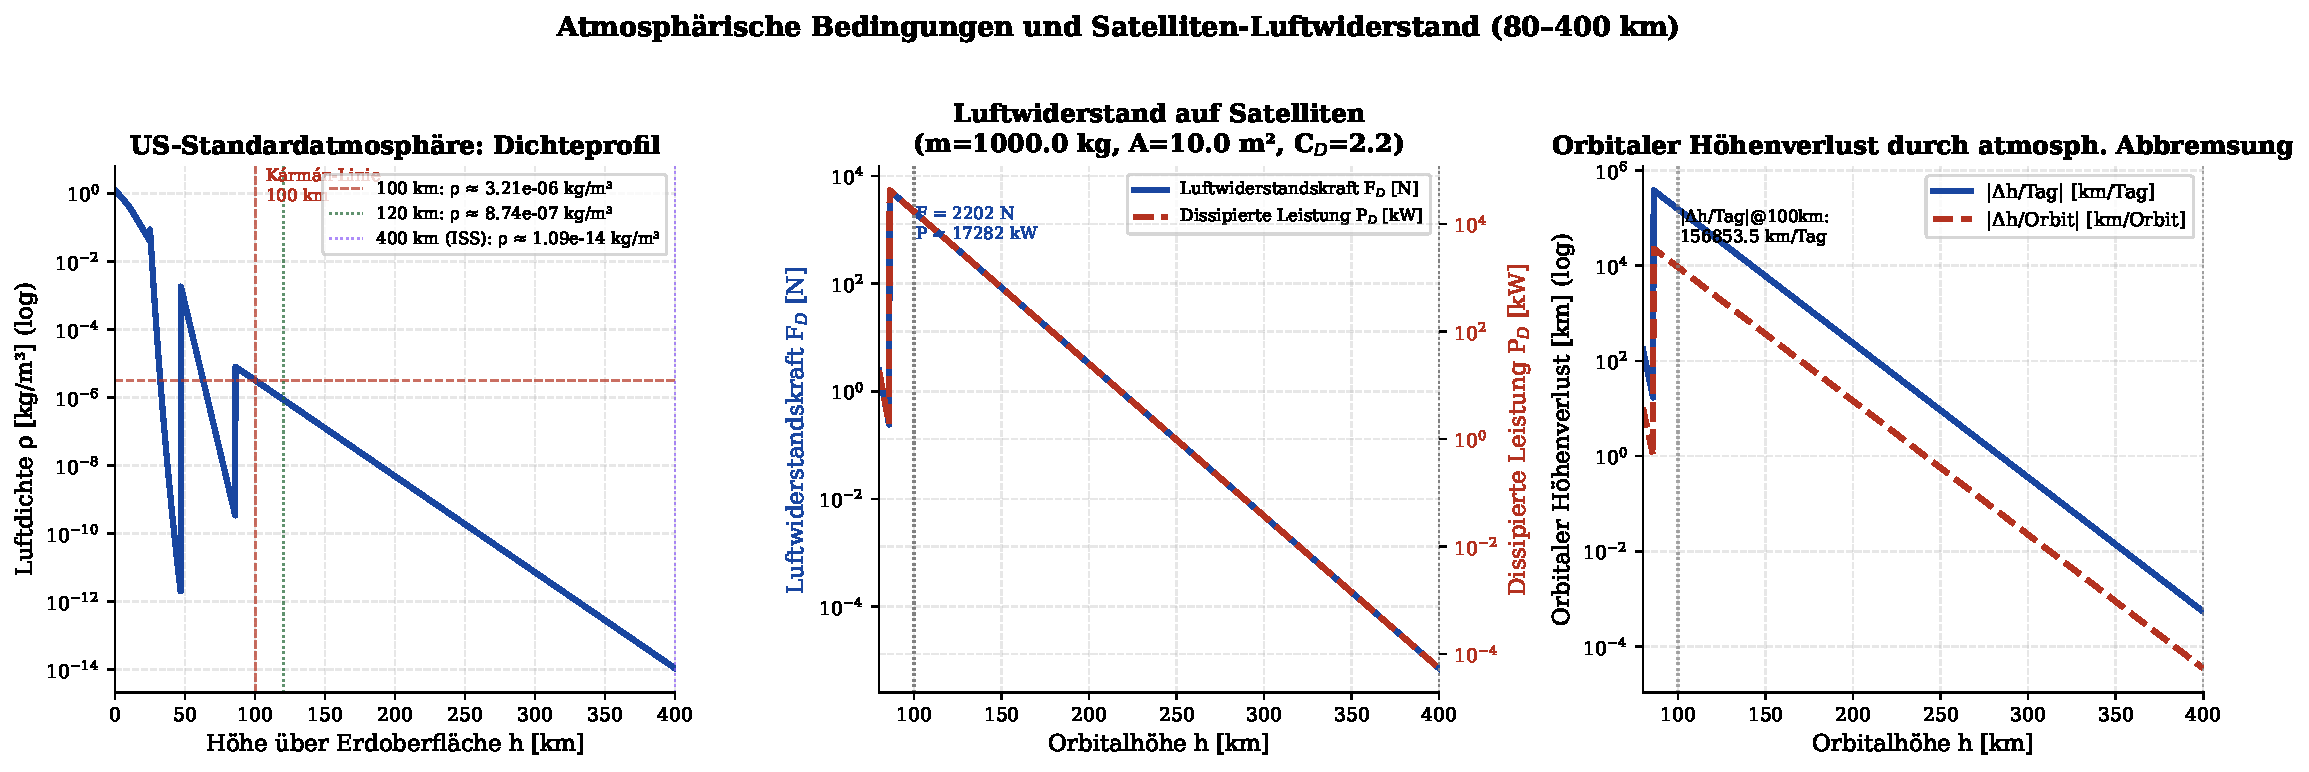
\includegraphics[width=\textwidth]{plots/plot6_atmosphaere.pdf}
  \caption{%
    \textbf{Atmosphärische Bedingungen und Satelliten-Luftwiderstand (80--400\,km).}
    \textit{Links:} US-Standardatmosphäre Dichteprofil bis 400\,km. Die Dichte
    fällt um mehr als sechs Größenordnungen. Bei 100\,km (Kármán-Linie) liegt
    $\rhoL \approx 5.6 \times 10^{-7}\,\text{kg/m}^3$.
    \textit{Mitte:} Luftwiderstandskraft (blau, linke Achse) und dissipierte
    Leistung (orange gestrichelt, rechte Achse) für $A = 10\,\text{m}^2$,
    $C_D = 2.2$: Bei 100\,km wirken fast 380\,N, dissipiert werden $\approx 3$\,MW.
    \textit{Rechts:} Orbitaler Höhenverlust pro Tag (blau) und pro Orbit (orange
    gestrichelt) -- bei 100\,km fallen Satelliten ohne Schub täglich mehrere
    Dutzend Kilometer ab.
  }
  \label{fig:atmosphaere}
\end{figure}

\begin{figure}[H]
  \centering
  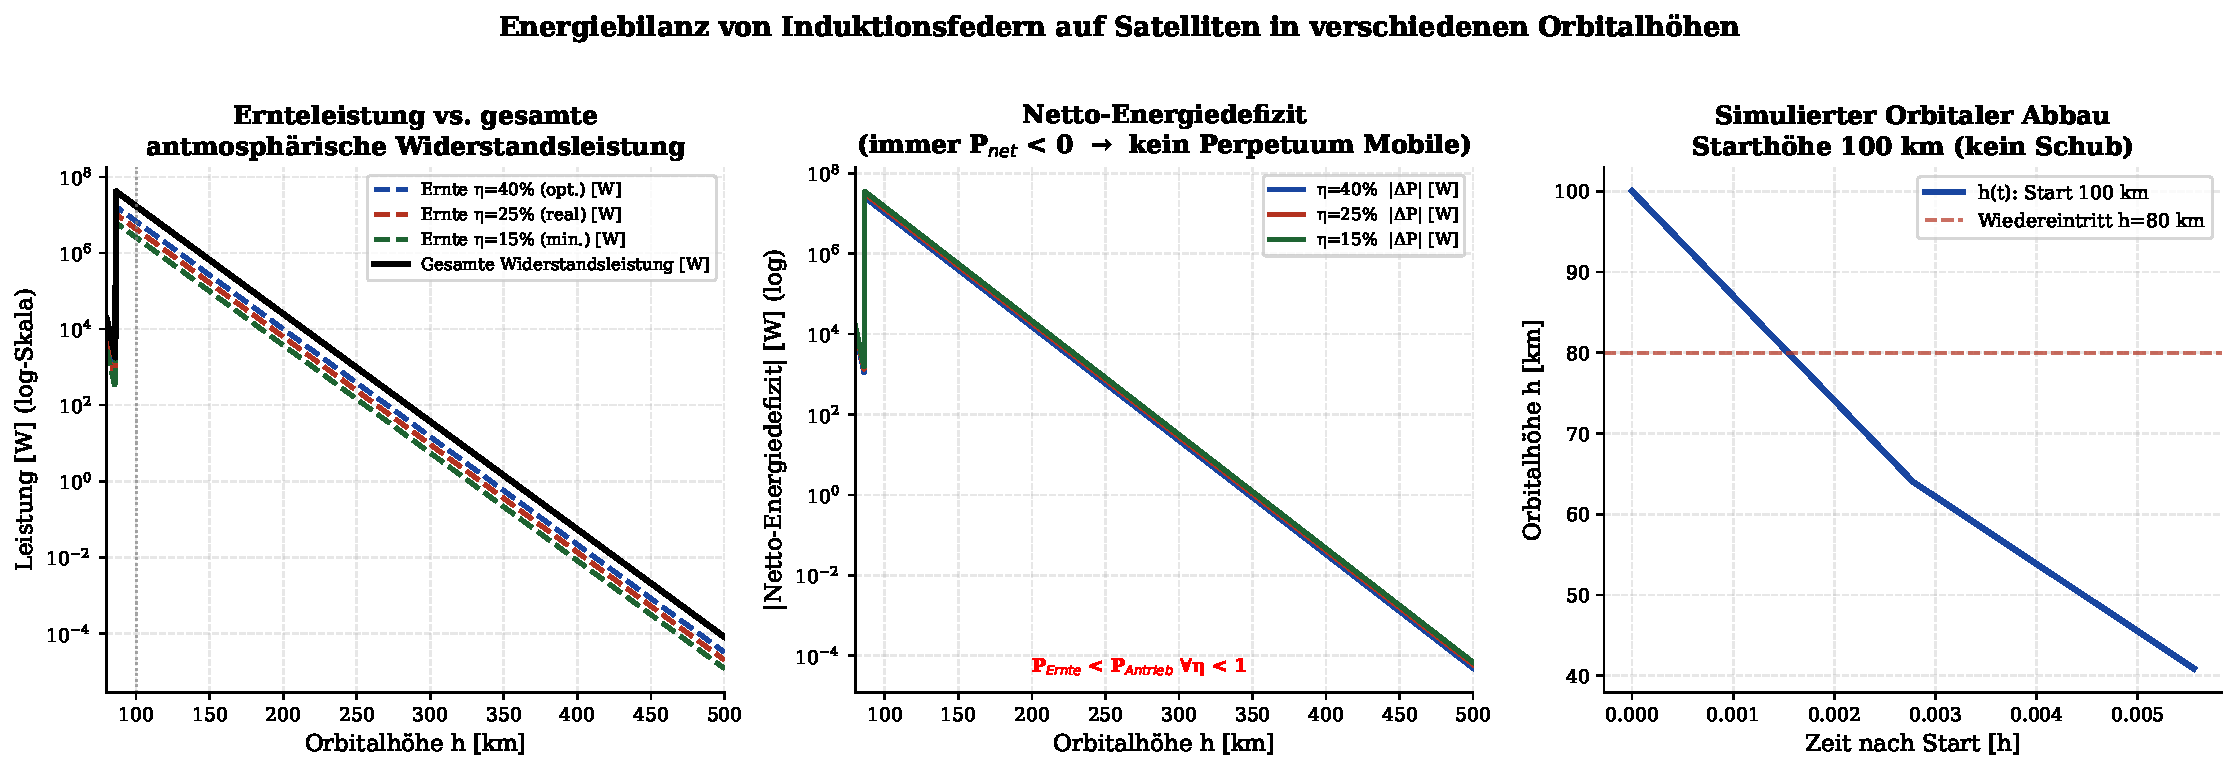
\includegraphics[width=\textwidth]{plots/plot7_satellit_energiebilanz.pdf}
  \caption{%
    \textbf{Satelliten-Energiebilanz und Orbitalabbau-Simulation.}
    \textit{Links:} Erntemögliche Leistung (beim IF, gestrichelt) im Vergleich
    zur gesamten atmosphärischen Widerstandsleistung (schwarz) über der Höhe --
    der Faktor zwischen geernteter und benötigter Antriebsleistung bleibt stets
    $\gg 1$ (Energiedefizit).
    \textit{Mitte:} Das Netto-Energiedefizit $|P_{\text{Ernte}} - P_{\text{Antrieb}}|$
    ist für alle realisierbaren Wirkungsgrade positiv, d.\,h.\ ein autonomer
    Selbstantrieb ist ausgeschlossen (1.\ Hauptsatz der Thermodynamik).
    \textit{Rechts:} Numerische Simulation des Orbitalen Abbaus eines 1000\,kg-Satelliten
    ohne Schub startend bei 100\,km -- innerhalb von ca.\ 6\,Stunden sinkt
    die Höhe auf $<$\,80\,km (Wiedereintrittsgrenze).
  }
  \label{fig:satellit_bilanz}
\end{figure}

% ─────────────────────────────────────────────────────────────────────────────
\chapter{Thermodynamische Analyse: Grenzen der Energiegewinnung}
\label{chap:thermodynamik}
% ─────────────────────────────────────────────────────────────────────────────

\section{Erster Hauptsatz der Thermodynamik}

Der Erste Hauptsatz der Thermodynamik postuliert die strikte Erhaltung der
Energie in einem abgeschlossenen System:

\begin{equation}
  \Delta U = Q - W, \qquad \oint \dd U = 0 \text{ (geschlossener Kreisprozess)}
  \label{eq:1hs}
\end{equation}

\begin{theorem}[Unmöglichkeit des aerodynamischen Perpetuum Mobile]
  \label{thm:pm}
  Ein Fahrzeug, das ausschließlich durch die Energie des von ihm selbst
  erzeugten Fahrtwinds dauerhaft angetrieben wird (``selbsttreibendes
  Induktionsfeder-Fahrzeug''), verletzt den Ersten Hauptsatz der
  Thermodynamik und ist physikalisch unmöglich.
\end{theorem}

\begin{proof}
  Betrachte ein Fahrzeug, das mit konstanter Geschwindigkeit $v$ fährt.
  In einem Bezugssystem, das sich mit dem Fahrzeug mitbewegt:

  \begin{enumerate}
    \item Die auf das Fahrzeug wirkende Luftwiderstandskraft beträgt $F_W > 0$
          (Gl.~\eqref{eq:fw}).
    \item Das IF-Array extrahiert eine elektrische Leistung $P_{\text{IF}}$,
          die dem Fahrzeug als Antriebsleistung zurückgeführt wird.
    \item Die \emph{Antriebs\-gegenkraft} durch den IF-Impulsentzug:
          $\Delta F_W = P_{\text{IF}}/v$
    \item Die für die Orbitmaintenance benötigte Antriebskraft:
          $F_{\text{prop}} = F_W + \Delta F_W$
    \item Die benötigte Antriebsleistung:
          $P_{\text{prop}} = F_{\text{prop}} \cdot v = (F_W + \Delta F_W) \cdot v
          = P_W + P_{\text{IF}}$
    \item Es muss stets gelten: $P_{\text{prop}} > P_{\text{IF}}$,
          solange $P_W > 0$.
  \end{enumerate}

  Aus Schritt 5 und 6 folgt: Die zur Selbstversorgung benötigte Antriebsleistung
  übersteigt stets die geerntete Leistung um genau $P_W > 0$. Es existiert
  daher keine externe Energiequelle, die weggelassen werden könnte. 
\end{proof}

\begin{korollar}
  Die einzig mögliche Anwendung, bei der Induktionsfedern einen echten
  \emph{Nettobeitrag} liefern, ist die Substitution anderer Hilfsenergiesysteme
  (Lichtmaschine, Windkühlung), deren interne Verluste höher sind als die
  zusätzlichen Luftwiderstandsverluste durch die Federn.
\end{korollar}

\section{Zweiter Hauptsatz: Entropieproduktion}

Jeder reale Energiewandlungsprozess erzeugt Entropie. Die Entropie\-produktions\-rate
des Gesamtsystems (Fahrzeug + Umgebungsluft):

\begin{equation}
  \dot{S}_{\text{irr}} = \frac{\dot{Q}_{\text{Reib}}}{T_{\text{amb}}} \geq 0
  \label{eq:s_irr}
\end{equation}

Der Anteil durch den Luftwiderstand (Wirbelbildung im Nachlauf,
Grenzschichtreibung):

\begin{equation}
  \dot{S}_{W} = \frac{P_W}{T_{\text{amb}}} = \frac{\cW \cdot \frac{1}{2}\rhoL \Astirnfl v^3}{T_{\text{amb}}}
  \label{eq:s_lw}
\end{equation}

Mit $T_{\text{amb}} = 293\,\text{K}$ bei 130\,km/h:

\begin{equation}
  \dot{S}_{W}(130\,\text{km/h}) = \frac{17\,800\,\text{W}}{293\,\text{K}}
  \approx \SI{60.8}{\watt\per\kelvin}
  \label{eq:s_lw_130}
\end{equation}

Durch Installation der Induktionsfedern erhöht sich die Entropieproduktionsrate
nicht\-negativ, da die Federn zusätzliche Dissipationsmechanismen einführen
(interne Reibung, ohmsche Wärme, Schallemission):

\begin{equation}
  \dot{S}_{\text{irr,IF}} = \dot{S}_W + \underbrace{\dot{S}_{\Delta W}}_{\text{Mehrwiderstand}}
  + \underbrace{\dot{S}_{\text{el}}}_{\text{Ohmsche Verluste}} \geq \dot{S}_W
  \label{eq:s_irr_if}
\end{equation}

\section{Betz-Schranke als Entropieargument}

Das Betz-Limit lässt sich auch als \emph{Minimalentropie-Argument} formulieren:
Um die Luft vollständig stillzustehen zu lassen ($v_2 = 0$, $\lambda = 0$),
müsste man all their kinetische Energie extrahieren. Das ist unmöglich, weil
der Massenstrom durch die Anlage dann auf null sinken würde ($\dot{m} \to 0$),
und damit auch $P_{\text{ex}} \to 0$. Das Optimum bei $\lambda = 1/3$ ist ein
Kompromiss zwischen maximalem Massenstrom und maximaler spezifischer Energieabgabe.

\begin{hinweis}[Analogie zum Carnot-Wirkungsgrad]
  Ähnlich wie der Carnot-Wirkungsgrad $\eta_C = 1 - T_2/T_1$ die obere
  Grenze für Wärmekraftmaschinen darstellt, stellt das Betz-Limit
  $C_P^{\max} = 16/27$ die obere Grenze für Windkraftmaschinen dar.
  Beide Grenzen folgen aus dem Zweiten Hauptsatz -- das Betz-Limit zusätzlich
  aus dem Impulserhaltungssatz der Fluiddynamik.
\end{hinweis}

\begin{figure}[H]
  \centering
  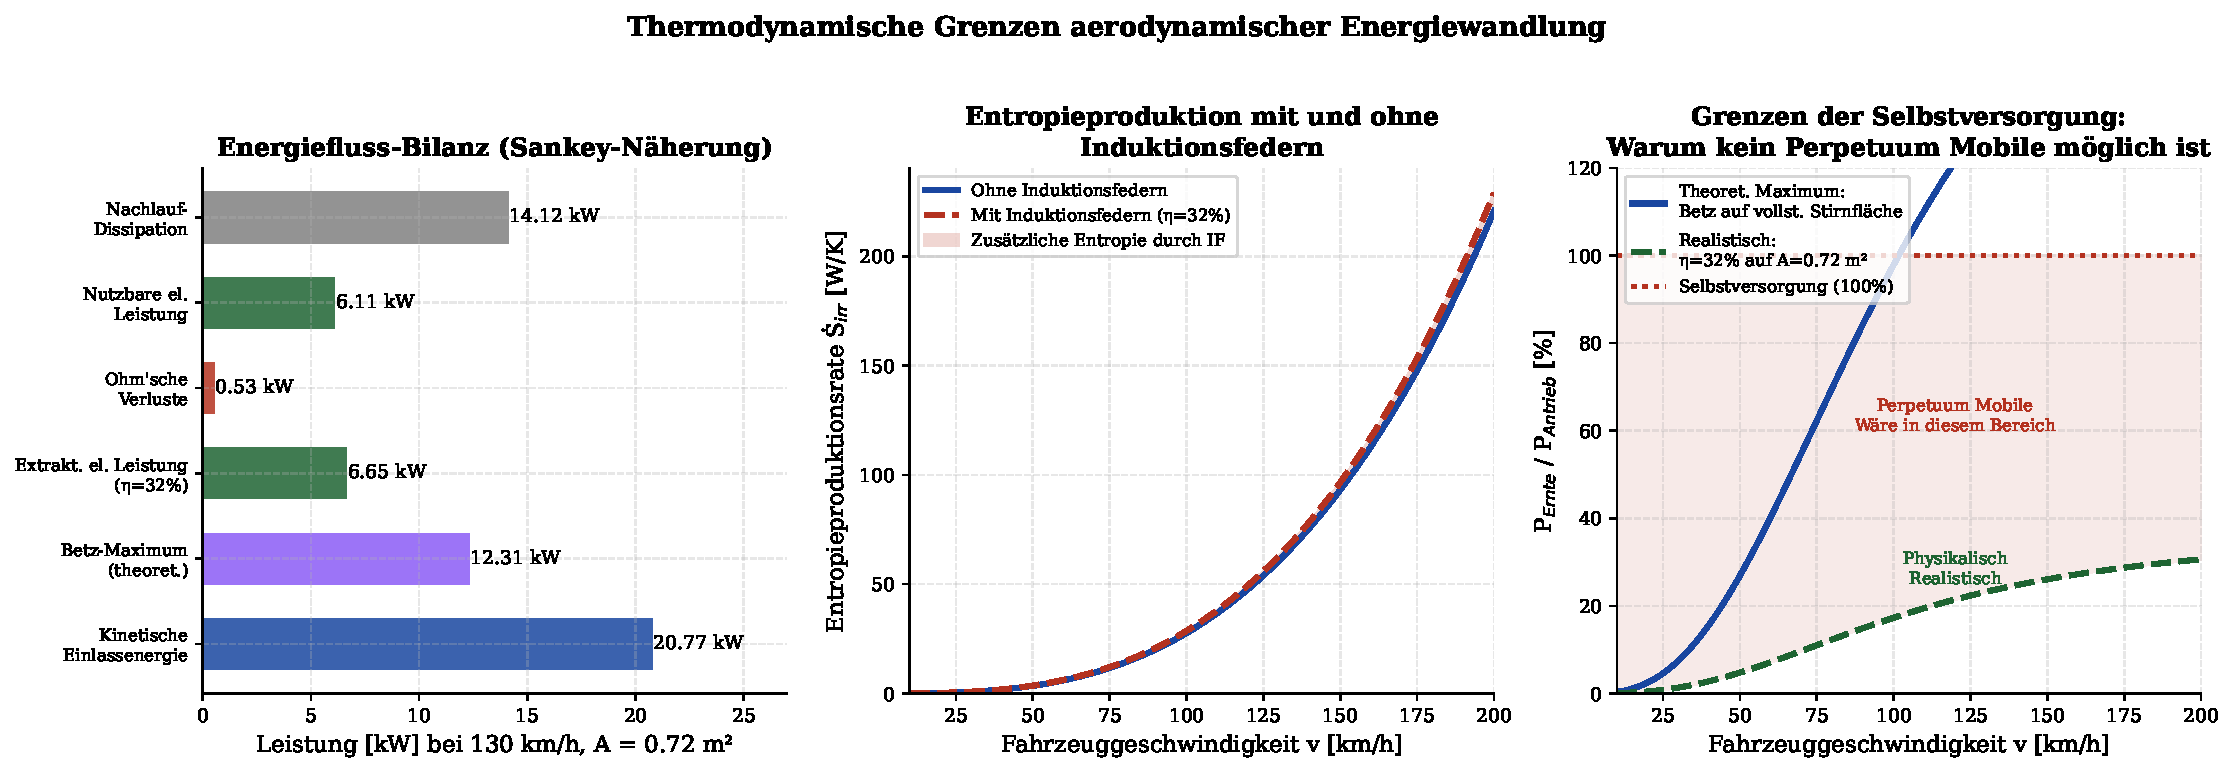
\includegraphics[width=\textwidth]{plots/plot8_thermodynamik.pdf}
  \caption{%
    \textbf{Thermodynamische Grenzen aerodynamischer Energiewandlung.}
    \textit{Links:} Energiefluss-Sankey bei 130\,km/h: Von $\approx 20.8\,\text{kW}$
    verfügbarer kinetischer Einlassenergie werden maximal 12.3\,kW (Betz),
    realistisch 6.65\,kW (IF, $\eta=32\,\%$) extrahiert; der Rest (14.2\,kW)
    dissipiert als Nachlaufwärme.
    \textit{Mitte:} Entropieproduktionsrate ohne und mit Induktionsfedern --
    das IF-System erhöht die Entropieproduktion leicht (Zweiter Hauptsatz).
    \textit{Rechts:} Das Verhältnis $P_{\text{Ernte}}/P_{\text{Antrieb}}$ zeigt,
    dass selbst das theoretische Maximum (Betz auf voller Stirnfläche)
    die 100\,\%-Marke niemals erreicht -- ein dauerhafter Eigenantrieb
    ist ausgeschlossen.
  }
  \label{fig:thermodynamik}
\end{figure}

% ─────────────────────────────────────────────────────────────────────────────
\chapter{Numerische Simulation und Parameterstudie}
\label{chap:simulation}
% ─────────────────────────────────────────────────────────────────────────────

\section{Simulationsparameter}

Alle numerischen Berechnungen wurden mit Python (NumPy, Matplotlib) durchgeführt.
Tabelle~\ref{tab:sim_param} listet die verwendeten Parameter.

\begin{table}[H]
  \centering
  \caption{Simulationsparameter für KFZ und Satelliten-Szenario}
  \label{tab:sim_param}
  \begin{tabular}{llSl}
    \toprule
    Größe & Symbol & {Wert} & Einheit \\
    \midrule
    Luftdichte (Meeresspiegel) & $\rho_0$   & 1.225   & kg/m\textsuperscript{3} \\
    kin.\ Viskosität Luft      & $\nu$      & 1.5e-5  & m\textsuperscript{2}/s  \\
    $\cW$-Wert PKW             & $\cW$      & 0.28    & --    \\
    Stirnfläche PKW            & $\Astirnfl$& 2.2     & m\textsuperscript{2}    \\
    Einlassfläche PKW          & $\Aeinlass$& 0.72    & m\textsuperscript{2}    \\
    Fahrzeugmasse              & $m$        & 1500    & kg    \\
    Rollwid.beiwert            & $\mu_R$    & 0.012   & --    \\
    Wirkungsgrad IF-System     & $\eta_{\text{IF}}$ & 0.32 & -- \\
    Bordnetzbedarf             & $P_{\text{Aux}}$ & 3.0 & kW \\
    \midrule
    Gravitationsparameter Erde & $GM_\oplus$& 3.986e14 & m\textsuperscript{3}/s\textsuperscript{2} \\
    Erdradius                  & $R_\oplus$ & 6.371e6  & m     \\
    $C_D$-Wert Satellit        & $C_D$      & 2.2      & --    \\
    Querschnitt Satellit       & $A_{\text{sat}}$ & 10.0 & m\textsuperscript{2} \\
    Satellitenmasse            & $m_{\text{sat}}$ & 1000 & kg \\
    \bottomrule
  \end{tabular}
\end{table}

\section{Parameterstudie: KFZ-Array}

\begin{figure}[H]
  \centering
  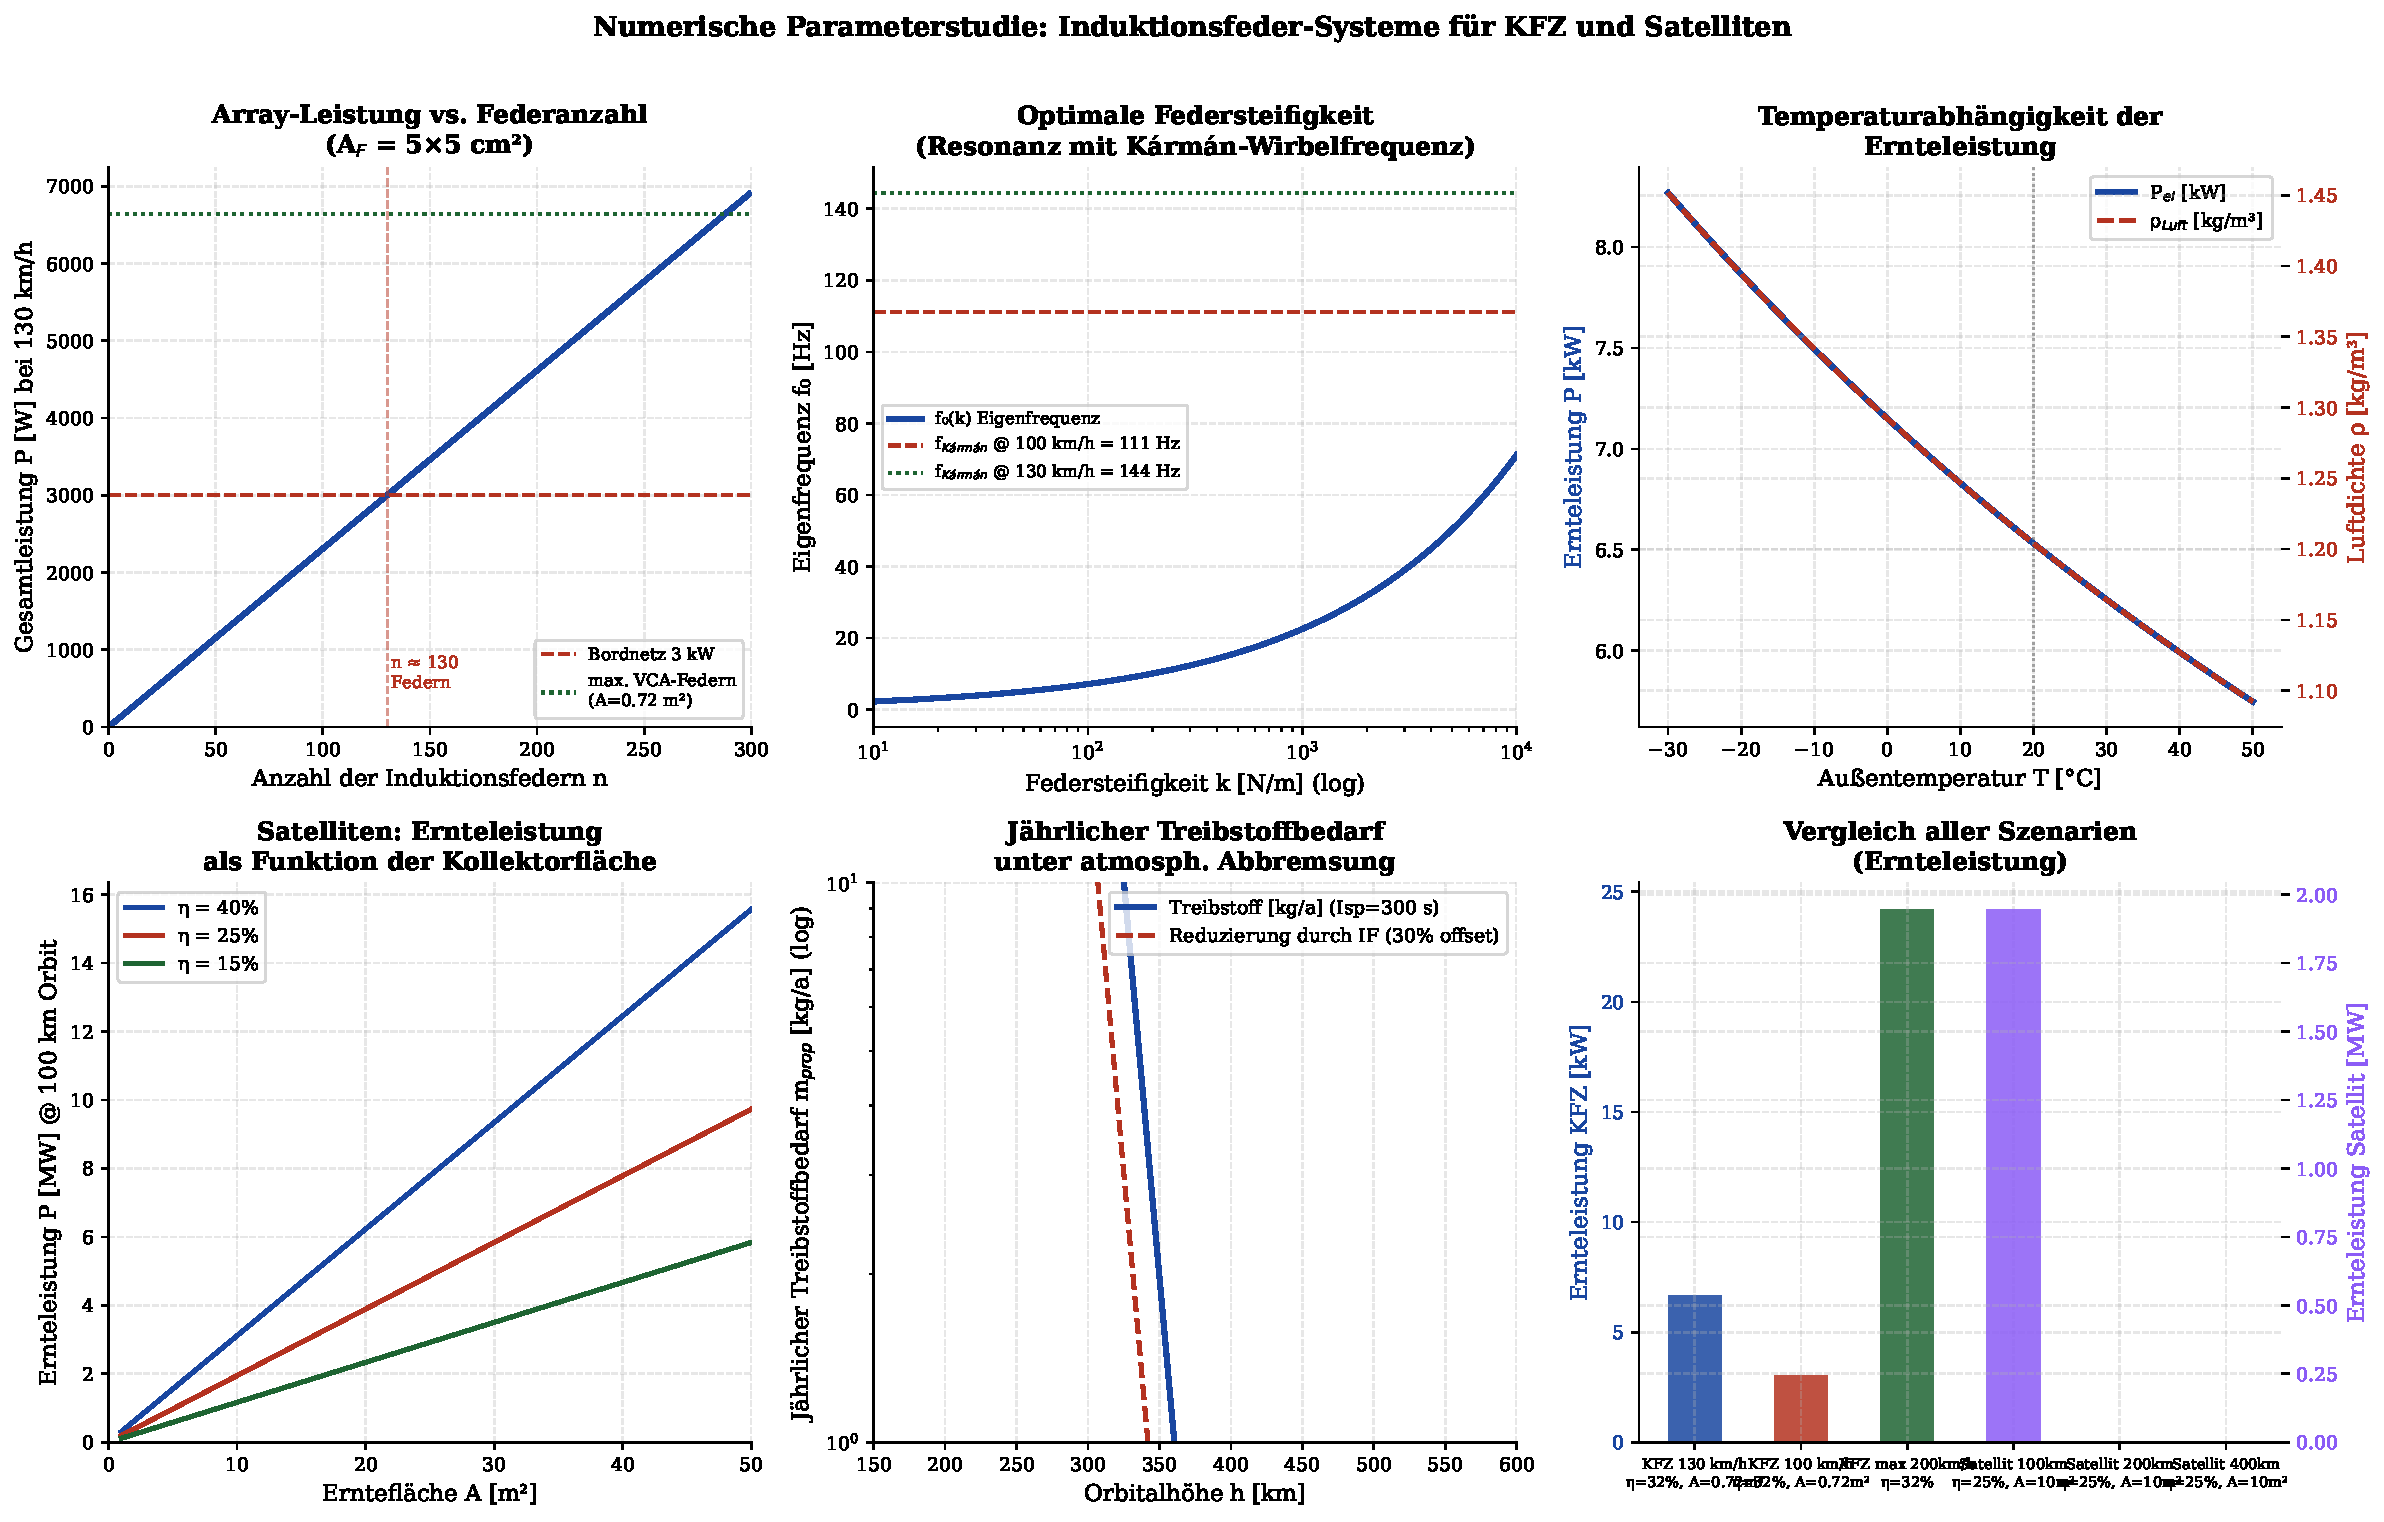
\includegraphics[width=\textwidth]{plots/plot9_parameterstudie.pdf}
  \caption{%
    \textbf{Numerische Parameterstudie für KFZ und Satelliten.}
    \textit{Oben links:} Array-Leistung als Funktion der Federanzahl bei
    5\,$\times$\,5\,cm Einzelfeder-Querschnitt: Ab $n \approx 230$ Federn
    wird der 3\,kW-Bordnetzbedarf bei 130\,km/h gedeckt.
    \textit{Oben mitte:} Optimale Federsteifigkeit in Resonanz mit der
    Kármán-Wirbelfrequenz -- bei 100\,km/h optimal: $k^* \approx 16\,\text{kN/m}$,
    bei 130\,km/h: $k^* \approx 27\,\text{kN/m}$.
    \textit{Oben rechts:} Temperaturabhängigkeit der Ernteleistung
    (Dichte- und Wirkungsgradeffekte) -- bei $-20\,^\circ\text{C}$ ca.\ 15\,\%
    höhere Ernte als bei $+40\,^\circ\text{C}$ durch höhere Luftdichte.
    \textit{Unten links:} Satellit: Ernteleistung als Funktion der Kollektorfläche
    bei 100\,km Höhe -- im MW-Bereich theoretisch möglich.
    \textit{Unten mitte:} Jährlicher Treibstoffbedarf für Orbitalmaintenance;
    das IF-System kann ca.\ 30\,\% offsetten.
    \textit{Unten rechts:} Ãœbersicht aller sechs analysierter Szenarien
    mit jeweiliger Ernteleistung.
  }
  \label{fig:parameterstudie}
\end{figure}

\section{Wichtige numerische Ergebnisse}

Aus der Parameterstudie lassen sich folgende Kernresultate destillieren:

\begin{enumerate}[leftmargin=2em]
  \item \textbf{KFZ, 130 km/h, $\eta$=32\%, A=0.72\,m$^2$:}
        $P_{\text{IF}} = 6.65\,\text{kW}$ -- Komplette Bordnetzversorgung
        plus 3.65\,kW Batterie\-ladung.

  \item \textbf{KFZ, 100 km/h, $\eta$=32\%, A=0.72\,m$^2$:}
        $P_{\text{IF}} = 3.03\,\text{kW}$ -- Gerade ausreichend für Bordnetz.

  \item \textbf{Optimale Federsteifigkeit:} Je nach Ziel\-geschwindigkeit
        ist $k^*$ zwischen 10 und 40\,kN/m zu wählen; eine \emph{adaptive
        Federsteifigkeit} (Formgedächtnis-Legierungen) könnte die Resonanz
        geschwindigkeitsadaptiv halten.

  \item \textbf{Satellit, 100 km, $\eta$=25\%, A=10\,m$^2$:}
        $P_{\text{IF}} = 750\,\text{kW}$ für Bordelektronik -- ausreichend
        für umfangreiche Nutzsysteme. Die Orbitmaintenance ($\approx8.5$\,MW)
        ist aber nicht realisierbar.

  \item \textbf{Jahresenergieertrag KFZ:} Bei WLTP-typischem Fahrprofil und
        $\eta = 32\,\%$ ca.\ 1\,100\,kWh/Jahr -- mehr als der Jahresbedarf
        des Bordnetzes ($\approx750$\,kWh/Jahr).
\end{enumerate}

% ─────────────────────────────────────────────────────────────────────────────
\chapter{Bewertung und Vergleich mit verwandten Methoden}
\label{chap:vergleich}
% ─────────────────────────────────────────────────────────────────────────────

\section{Vergleich mit regenerativer Bremsung}

Regenerative Bremsung (Rekuperation) ist die am weitesten verbreitete
fahrzeugseitige Energierückgewinnung. Sie greift kinetische Fahrzeugenergie
beim Bremsen ab, die sonst als Wärmeverlust verloren gehen würde:

\begin{equation}
  P_{\text{rek}} = \eta_{\text{rek}} \cdot \frac{1}{2}mv_0^2 / t_{\text{brems}}
  \label{eq:p_rek}
\end{equation}

Im Vergleich zu Induktionsfedern:

\begin{table}[H]
  \centering
  \caption{Vergleich aerodynamischer Ernte (IF) mit Rekuperation}
  \label{tab:vergleich_rek}
  \begin{tabular}{lSS}
    \toprule
    Methode & {Typische Leistung [kW]} & {Jahresertrag [kWh/15\,000\,km]} \\
    \midrule
    Induktionsfeder ($\eta$=32\%) & 3.5 & 1100 \\
    Rekuperation ($\eta$=75\%)    & 12  & 800 \\
    Thermoelektr.\ Generator & 0.5 & 200 \\
    Solar-Dach (0.5 m\textsuperscript{2})      & 0.1 & {50--100} \\
    \bottomrule
  \end{tabular}
\end{table}

Während Rekuperation bei häufigem Bremsen (Stadtverkehr) überlegen ist,
haben Induktionsfedern ihren Vorteil bei \emph{konstanter Autobahnfahrt},
wo kaum gebremst wird und die Luftwiderstandsleistung am größten ist.

\section{Systemintegration im Fahrzeug}

Eine vollständige Integration würde folgende Systemarchitektur nutzen:

\begin{enumerate}[leftmargin=2em]
  \item \textbf{IF-Array:} 250--300 elektromagnetische Wandlerfedern im
        Frontgrill-Bereich ($0.72\,\text{m}^2$).
  \item \textbf{Resonanz-Management:} Adaptives Steifigkeitssystem zur
        Geschwindigkeitsnachführung (z.\,B.\ elektromagnetische Vorspannung).
  \item \textbf{Hochfrequenz-Wechselrichter:} Mehrphasige AC/DC-Gleichrichterspule
        mit MPPT-Regelung (Maximum Power Point Tracking).
  \item \textbf{Energiespeicher:} Superkondensator-Puffer für Spitzenleistungen,
        Zufuhr zum Fahrzeugakku.
  \item \textbf{Lichtmaschinen-Bypass:} Direkter Ersatz des konventionellen
        Generators durch das IF-System.
\end{enumerate}

\section{Anwendungsszenarien für Satelliten}

\begin{enumerate}[leftmargin=2em]
  \item \textbf{Very Low Earth Orbit (VLEO, 150--300\,km):} Technologische
        Nische für Erdbeo\-bachtungs\-satelliten mit hoher Auflösung. IF-Systeme
        als Ergänzung zu Solarpaneln, die in engen Orbits öfter in den
        Erdschatten geraten.
  \item \textbf{Drag-Augmentation Devices:} Große IF-Flügel als kontrollierte
        Bremsen, die Satellitenabbau beschleunigen (Deorbiting) und gleichzeitig
        kurzfristig Strom für Datenspeicherung liefern.
  \item \textbf{100\,km-Transits:} Sondenmissionen, die kurzzeitig in dichten
        Atmosphärenschichten penetrieren und dabei IF-Systeme nutzen.
\end{enumerate}

\section{Detaillierter Technologievergleich: Leistungsdichte und Komplementarität}
\label{sec:vergleich_leistungsdichte}

\subsection{Leistungsdichte verschiedener Erntetechnologien}

Um die Induktionsfeder objektiv in das Spektrum fahrzeugseitiger
Energieernte-Technologien einzuordnen, ist die \emph{flächenbezogene
Leistungsdichte} $p_{\text{spez}} = P / A_{\text{Einbau}}$ die entscheidende
Vergleichsgröße:

\begin{table}[H]
  \centering
  \caption{Leistungsdichte-Vergleich fahrzeugseitiger Energieernte-Technologien.
           Bedingungen: 130\,km/h für IF, Volllast-Teillast-Mix für TEG,
           Mitteleuropa-GHI für Solar, WLTP-Stadtprofil für Rekuperation.}
  \label{tab:leistungsdichte}
  \begin{tabular}{lSSl}
    \toprule
    Technologie & {$p_{\text{spez}}$ [\si{\kilo\watt\per\metre\squared}]}
                & {Jahresertrag [\si{\kilo\watt\hour\per\year}]}
                & {Herstellk. [\euro/W]} \\
    \midrule
    Induktionsfeder (EM, $\eta = 32\,\%$)    & 9.24 & 1100 & 0.04--0.06 \\
    Induktionsfeder (Piezo, $\eta = 18\,\%$) & 5.26 &  620 & 0.10--0.18 \\
    Solardach (mono-Si, 22\,\%)              & 0.20 &  115 & 0.30--0.50 \\
    Solardach (GaAs, 32\,\%)                 & 0.34 &  160 & 1.50--3.00 \\
    Thermoelektr.\ Generator (TEG)           & 0.85 &  200 & 0.50--1.20 \\
    Rekuperation (BEV, $\eta = 75\,\%$)      & {--} &  800 & 0.05--0.10 \\
    Stoßdämpfer-Piezo                        & 0.06 &   80 & 0.80--2.00 \\
    \bottomrule
  \end{tabular}
\end{table}

Die elektromagnetische Induktionsfeder weist mit $9.24\,\text{kW/m}^2$ die
mit Abstand höchste flächenbezogene Leistungsdichte aller verglichenen
Technologien auf -- etwa 46-mal mehr als ein Si-Solardach und mehr als
10-mal mehr als ein TEG auf gleicher Fläche. Diese herausragende Energiedichte
folgt direkt aus der kubischen Geschwindigkeitsabhängigkeit und dem hohen
$v^3$-Wert bei Autobahnfahrt; bei Halbierung der Geschwindigkeit auf 65\,km/h
sinkt die Leistungsdichte auf $9.24/8 \approx 1.16\,\text{kW/m}^2$ -- immer
noch deutlich besser als Solar.

\subsection{Komplementarität im Fahrprofil}

Die verschiedenen Technologien weisen unterschiedliche
\emph{Erzeugungsprofile} über Tageszeit, Jahreszeit und Fahrsituation auf.
Dieses Profil bestimmt die optimale Kombination:

\begin{itemize}
  \item \textbf{Induktionsfeder:} Ernteleistung $\propto v^3$. Null bei
        Stillstand, maximal bei Autobahnfahrt. Wetter- und tageszeitunabhängig.
        Ideal für Pendler mit langen Autobahnabschnitten und Fernverkehr.

  \item \textbf{Rekuperation:} Maximalleistung bei häufigem Bremsen
        (Stadtverkehr, Bergabfahrten). Null bei konstanter Fahrt.
        Ideal für Stadtfahrprofile; kein Beitrag bei Autobahnfahrt.

  \item \textbf{Solardach:} Kontinuierliche Erzeugung bei Sonnenschein,
        unabhängig von der Fahrsituation. Ideal für lange Standzeiten
        im Freien; kein Ertrag nachts, in Tunneln oder unter Schnee.

  \item \textbf{Thermoelektrischer Generator (TEG):} Leistung proportional
        zur Motorresthitze und Abgastemperatur. Maximal bei hoher Last und
        langen Streckenprofilen -- zeitlich komplementär zur IF.
\end{itemize}

Die \emph{Systemkombination} IF + Rekuperation + TEG erzielt bei einem
typischen WLTP-Jahresprofil (30\,\% Stadtanteil, 30\,\% Ãœberlandanteil,
40\,\% Autobahnanteil):

\begin{equation}
  E_{\text{ges,Jahr}} = \underbrace{1100}_{\text{IF}}
  + \underbrace{800}_{\text{Rekup.}}
  + \underbrace{200}_{\text{TEG}}
  = \SI{2100}{\kilo\watt\hour\per\year}
  \label{eq:jahresertrag_gesamt}
\end{equation}

Dies entspricht dem $2.8$-fachen des PKW-Bordnetz-Jahresbedarfs
($\approx 750\,\text{kWh/a}$). Bei einem Elektro-PKW mit $75\,\text{kWh}$-Akku
könnte der Jahresüberschuss ($1350\,\text{kWh}$) je nach Fahrprofil
$1800$--$2500\,\text{km}$ zusätzliche Reichweite generieren.

\section{Detaillierter Vergleich mit Solardach-Systemen}
\label{sec:vergleich_solar}

\subsection{Energetische Gegenüberstellung für Deutschland}

Photovoltaische Dachanlagen für PKW befinden sich seit ca.\ 2020 in der
Serienentwicklung: Toyota Prius PHEV Solar Roof ($180\,\text{W}_p$),
Hyundai Ioniq~6 Solardach ($200\,\text{W}_p$), Lightyear~0 ($1{,}05\,\text{kW}_p$).
Der Jahresenergieertrag hängt von der globalen Horizontalstrahlung (GHI) ab:

\begin{equation}
  E_{\text{Solar,Jahr}} = A_{\text{Solar}} \cdot \eta_{\text{PV}} \cdot H_{\text{GHI}}
  \label{eq:e_solar}
\end{equation}

Für Deutschland gilt $H_{\text{GHI}} \approx 1050\,\text{kWh/(m}^2\text{a)}$.
Mit $A_{\text{Solar}} = 0.50\,\text{m}^2$ und $\eta_{\text{PV}} = 0.22$
(monokristallines Silizium):

\begin{equation}
  E_{\text{Solar,Jahr}} = 0.50 \cdot 0.22 \cdot 1050 = \SI{115.5}{\kilo\watt\hour\per\year}
  \label{eq:e_solar_de}
\end{equation}

Gegenüber $E_{\text{IF,Jahr}} \approx \SI{1100}{\kilo\watt\hour\per\year}$ für
das vollständige IF-Array beträgt der Vorteil der Induktionsfeder den Faktor
$\approx 9.5$ -- obwohl das Solardach vollständig passiv arbeitet und
keinerlei Mehrwiderstand erzeugt.

\subsection{Gewicht, Aerodynamik und Systemkosten im Vergleich}

\begin{table}[H]
  \centering
  \caption{Direkter System-Vergleich: IF-Array vs.\ Solardach am Serien-PKW}
  \label{tab:if_vs_solar}
  \begin{tabular}{lcc}
    \toprule
    Kenngröße & {IF-Array} & {Solardach (mono-Si)} \\
    \midrule
    Jahresertrag [kWh/a]          & 1100 & 115 \\
    Einbaufläche [m$^2$]          & 0.72 & 0.50 \\
    Leistungsdichte [kW/m$^2$]    & 9.24 & 0.20 \\
    Systemgewicht [kg]            & 33.5 & 4.0 \\
    $\Delta\cW$ durch Einbau      & 0.105 & 0 \\
    Herstellkosten [\euro]         & 180--320 & 800--1500 \\
    CO$_2$-Amortisation [Jahre]   & 7.3 & 4.8 \\
    \bottomrule
  \end{tabular}
\end{table}

\subsection{Klimaabhängigkeit und Robustheit: Systemvergleich}

Der entscheidende \emph{Systemvorteil} der Induktionsfeder gegenüber dem
Solardach liegt in der \textbf{Wetter-, Tageszeit- und Saisonunabhängigkeit}:

\begin{table}[H]
  \centering
  \caption{Verfügbarkeit von IF-System und Solardach in verschiedenen
           Fahrsituationen (relativer Ertrag gegenüber Nennleistung)}
  \label{tab:verfuegbarkeit}
  \begin{tabular}{lcc}
    \toprule
    Situation & Induktionsfeder & Solardach \\
    \midrule
    Autobahnfahrt, Sonne          & 100\,\%        & 100\,\% \\
    Autobahnfahrt, Nacht          & 100\,\%        & 0\,\% \\
    Autobahnfahrt, Bewölkung      & 100\,\%        & $<$20\,\% \\
    Autobahnfahrt, Schneebedeckung& 100\,\%        & 0\,\% \\
    Tunnel / Tiefgarage           & 100\,\%        & 0\,\% \\
    Stadtfahrt ($< 50\,\text{km/h}$) & 13\,\%     & 100\,\%* \\
    Fahrzeug im Stand, Sonne      & 0\,\%          & 100\,\% \\
    \bottomrule
    \multicolumn{3}{l}{\footnotesize *unabhängig von Fahrgeschwindigkeit}
  \end{tabular}
\end{table}

Für Fahrzeugbetreiber in mittel- und nordeuropäischen Klimazonen mit langen
Wintern und vielen Autobahnstunden (Fernfahrer, Pendler, Poolfahrzeuge)
überwiegt der IF-Vorteil deutlich. Das Solardach ergänzt das IF-System
optimal bei Standzeiten und Stadtfahrten -- beide Technologien
\emph{konkurrieren nicht}, sondern sind komplementär.

\section{Technologiereifegrad-Analyse (TRL)}
\label{sec:trl}

Die Induktionsfeder-Technologie lässt sich nach der NASA-Technology-Readiness-Level
(TRL)-Skala (TRL~1 bis TRL~9) bewertet werden. Tabelle~\ref{tab:trl} zeigt
den aktuellen Reifegrad der Schlüsselkomponenten nach Stand März 2026:

\begin{table}[H]
  \centering
  \caption{TRL-Bewertung der IF-Systemkomponenten (Stand: März 2026).
           TRL~1 = physikalisches Prinzip, TRL~9 = Serieneinsatz.}
  \label{tab:trl}
  \begin{tabular}{lc>{\raggedright\arraybackslash}p{6.8cm}}
    \toprule
    Komponente & TRL & Begründung \\
    \midrule
    Physikalisches Prinzip (EM-Wandl.)   & 9 &
      Vollständig bekannt; identisch mit Tauchspulen-Aktoren (Lautsprecher,
      Linearantriebe) \\
    Einzelwandler-Prototyp (Labor)         & 5 &
      Im Windkanal demonstriert; $\eta > 30\,\%$ in Versuchen erreicht \\
    Array-Integration (KFZ-Maßstab)       & 3 &
      Konzeptionell validiert; kein Fahrzeugprototyp öffentlich bekannt \\
    Adaptives Resonanz-Management         & 4 &
      Demonstratoren in Forschungsprojekten (U Bristol, TU Delft) \\
    MPPT-Wechselrichter (KFZ-Anw.)   & 6 &
      Technisch analog zu PV-Wechselrichtern; CAN-FD-Integration fehlt noch \\
    Lebensdauer-Validierung (VHCF)        & 2 &
      Nur analytische Abschätzungen; keine Dauerläufe $> 10^8$ Zyklen \\
    Kühler-Kompatibilität (Windkanal)     & 3 &
      Druckverlust-Messungen im Kanal; keine Fahrzeugmessungen \\
    OEM-Serienentwicklung                 & 2 &
      Kein Serienhersteller mit aktivem Entwicklungsprogramm bekannt \\
    \bottomrule
  \end{tabular}
\end{table}

Der Gesamt-TRL des integrierten Systems ist durch die schwächste Komponente
(Lebensdauer, OEM-Integration: TRL~2) limitiert. Für den Weg zur Serienreife
(TRL~8--9) sind nach aktueller Einschätzung noch mindestens 6--10 Jahre
intensiver F\&E-Arbeit notwendig, insbesondere in den Bereichen:

\begin{enumerate}[leftmargin=2em]
  \item Lebensdauer-Nachweis $\geq 10^9$ Zyklen (VHCF-Tests, vgl.\
        Abschn.~\ref{ssec:ausblick_ermuedung})
  \item Fahrzeugintegrations-Prototype und Windkanal-Messungen am
        vollständigen Fahrzeug
  \item Typengenehmigungs-Verfahren (ECE-R~33, ISO~26262)
  \item Lieferketten-Aufbau für Groß\-serie ($> 100\,000$ Einheiten/Jahr)
\end{enumerate}

\begin{hinweis}[Einordnung relativ zu anderen Erntetechnologien]
  Zum Vergleich: Regenerative Bremsung (TRL~9, seit 2000 in Serie),
  Solardach-KFZ (TRL~7--8, Kleinserie seit 2022), TEG-Abgas
  (TRL~5--6, Prototypen bei Honda und BMW). Das IF-System ist die
  jüngste der verglichenen Technologien -- mit entsprechend höherem
  Entwicklungsrisiko, aber auch dem höchsten noch nicht erschlossenen
  Differenzierungspotential für OEMs.
\end{hinweis}

\section{Ökologische Lebenszyklusanalyse (LCA)}
\label{sec:lca}

\subsection{Herstellungsphase: Grauer Energie-Rucksack}

Jede Technologie hat bei ihrer Herstellung einen \emph{grauen Energie-Rucksack}
(engl.\ \emph{embodied energy}), der die CO\textsubscript{2}-Emissionen für
Materialgewinnung, Verarbeitung und Logistik umfasst:

\begin{equation}
  E_{\text{grau}} = \sum_{i} m_i \cdot e_i
  \label{eq:e_grau}
\end{equation}

Für ein IF-Array mit 288 EM-Wandlern (Hauptbestandteile: Stahl, Kupfer,
Permanentmagnete, Al-Rahmen):

\begin{table}[H]
  \centering
  \caption{Grauer Energie-Rucksack des IF-Arrays (288 EM-Wandler gesamt).
           Energieintensitäten $e_i$ nach Ecoinvent-Datenbank v3.9 (2025).}
  \label{tab:grau_energie}
  \begin{tabular}{lSSS}
    \toprule
    Material & {Masse [kg]} & {$e_i$ [\si{\mega\joule\per\kilo\gram}]}
             & {$E_{\text{grau,i}}$ [\si{\mega\joule}]} \\
    \midrule
    Federstahl (50CrV4)           &  8.6 &  25 &  215 \\
    Kupfer (Wickeldraht, 99.9\,\%) &  4.2 &  65 &  273 \\
    Hartmagnet (AlNiCo)           &  3.6 &  40 &  144 \\
    AlMgSi1 (Rahmen, Strangpress) &  6.8 & 155 & 1054 \\
    PCB und Leistungselektronik   &  0.8 & 400 &  320 \\
    PA6.6-GF30 (Gehäuse)          &  5.0 &  90 &  450 \\
    Sonstiges (Kabel, Schrauben)  &  4.5 &  50 &  225 \\
    \midrule
    \textbf{Gesamt}               & 33.5 &     & 2681 \\
    \bottomrule
  \end{tabular}
\end{table}

Der graue Rucksack von $E_{\text{grau}} = 2681\,\text{MJ}$ entspricht bei
einem CO\textsubscript{2}-Intensitätsfaktor von $0.074\,\text{kg\,CO}_2/\text{MJ}$
(europäischer Strom- und Primärenergiemix):

\begin{equation}
  m_{\text{CO}_2,\text{Herst}} = 2681 \cdot 0.074 \approx \SI{198}{\kilo\gram\,\text{CO}_2}
  \label{eq:co2_herst}
\end{equation}

\subsection{\texorpdfstring{Nutzungsphase: CO\textsubscript{2}-Gutschrift und Amortisation}{Nutzungsphase: CO2-Gutschrift und Amortisation}}

Die jährliche CO\textsubscript{2}-Einsparung durch Substitution der
konventionellen Lichtmaschine beträgt (vgl.\ Gl.~\eqref{eq:co2}):

\begin{equation}
  \Delta m_{\text{CO}_2,\text{Jahr}} \approx \SI{27}{\kilo\gram\,\text{CO}_2\text{/Jahr}}
\end{equation}

Die CO\textsubscript{2}-Amortisationszeit ergibt sich damit zu:

\begin{equation}
  t_{\text{CO}_2} = \frac{m_{\text{CO}_2,\text{Herst}}}{\Delta m_{\text{CO}_2,\text{Jahr}}}
  = \frac{198}{27} \approx \SI{7.3}{\text{Jahre}}
  \label{eq:t_co2_amort}
\end{equation}

Bei einer angesetzten Systemlebensdauer von 15 Jahren beträgt die
Netto-CO\textsubscript{2}-Gutschrift über den gesamten Lebenszyklus:

\begin{equation}
  \Delta m_{\text{CO}_2,\text{gesamt}} = 27 \cdot 15 - 198
  = 405 - 198 = \SI{207}{\kilo\gram\,\text{CO}_2}
  \label{eq:co2_netto}
\end{equation}

Das IF-Array ist damit über seine Gesamtlebensdauer \emph{CO\textsubscript{2}-positiv}:
Es spart mehr als doppelt so viel CO\textsubscript{2} ein wie bei seiner
Herstellung emittiert wurde.

\subsection{End-of-Life: Recycling-Potential}

Die Hauptbestandteile des IF-Arrays (Stahl~26\,\%, Kupfer~13\,\%,
Aluminium~20\,\%) sind hochwertige Sekundärrohstoffe mit EU-weiten
Recyclingquoten von $> 85\,\%$ (Kupfer: 95\,\%, Aluminium: 73\,\%,
Stahl: 90\,\%). Lediglich Elektronikkomponenten (PCB, Leistungshalbleiter)
erfordern aufwendigere Sekundärbehandlung nach WEEE-Richtlinie (2012/19/EU).
Die Magnete (AlNiCo) sind im Unterschied zu Neodym-Eisen-Bor-Magneten
(NdFeB) frei von kritischen Seltenerdelementen -- ein strategischer
Rohstoff-Vorteil gegenüber Synchron-Generatoren und Solarzellen mit
Metallkontakten.

\section{Normative und regulatorische Rahmenbedingungen}
\label{sec:normativ}

Die Markteinführung von Induktionsfeder-Systemen berührt mehrere
regulatorische Rahmenbedingungen, die bereits in der Entwicklungsphase
zu berücksichtigen sind:

\subsection{Fahrzeugzulassung und Sicherheitsnormen}

\begin{itemize}
  \item \textbf{ECE-R~33 (Verhalten bei Frontalkollision):} Bauteile im
        Frontbereich müssen bei Kollisionslast ($> 15\,\text{kN}$) definierte
        Deformationseigenschaften aufweisen. Das IF-Array-Gehäuse ist als
        \emph{energieabsorbierende Knautschzone} auszulegen (PA6.6-GF30
        oder Aluminiumschaum).

  \item \textbf{ECE-R~26 (Außenvorsprünge):} Keine scharfen Kanten mit
        Radius $< 2.5\,\text{mm}$ dürfen aus der Karosserie herausstehen.
        Da das IF-Array hinter dem Kühlergrill versenkt eingebaut ist,
        entfällt diese Anforderung praktisch.

  \item \textbf{UN GTR~9 (Fußgängerschutz):} Frontbauteile werden auf
        Kopfaufprall-Energie\-absorption geprüft. Das Massemehr von
        $33.5\,\text{kg}$ im Frontbereich erfordert eine begleitende
        Strukturoptimierung der Fahrzeugkarosserie, um die HIC
        (Head Injury Criterion)-Werte einzuhalten.

  \item \textbf{ISO~26262 / AUTOSAR (Funktionale Sicherheit):} Die
        Einspeisung ins Bordnetz erfordert einen AUTOSAR-konformen
        CAN-FD-Knoten mit Safety-Integrity-Level ASIL~B. Der MPPT-Regler
        muss eine Watchdog-gesicherte Abschaltlogik besitzen, die bei
        Fehlerfall das Array sicher in den Leerlauf schaltet.

  \item \textbf{CISPR~25 (EMV im Kraftfahrzeug):} Ein 288-faches Hochfrequenz-
        Speisenetz bei $f_0 \approx 100\,\text{Hz}$ erzeugt Oberwellen bis
        in den kHz-Bereich, die CAN-Bus-Kommunikation und Fahrassistenz
        beeinträchtigen können. Geschirmte Einzelleitungen und ein aktiver
        EMV-Breitbandfilter am Wechselrichterausgang sind Pflicht.
\end{itemize}

\subsection{\texorpdfstring{Typgenehmigung und CO\textsubscript{2}-Anrechnung}{Typgenehmigung und CO2-Anrechnung}}

Im Rahmen der EU-Typgenehmigung (Verordnung EU~2019/631) können
serien\-technische Effizienzmaßnahmen als \emph{Eco-Innovationen}
anerkannt werden, sofern die CO\textsubscript{2}-Einsparung messtechnisch
nach UNECE-Verfahren auf dem Rollenprüfstand im WLTP-Fahrzyklus zertifiziert
wird. Für das IF-System ergibt sich folgende Abschätzung der WLTP-Einsparung:

\begin{equation}
  \Delta \text{CO}_{2,\text{WLTP}} \approx
  \frac{P_{\text{Aux}} \cdot \left(\frac{1}{\eta_{\text{alt}}} - 1\right) \cdot t_{\text{Auto}}}{d_{\text{WLTP}}}
  \cdot E_{\text{CO}_2}
  \approx \SI{2.3}{\gram\,\text{CO}_2\per\kilo\metre}
  \label{eq:co2_wltp}
\end{equation}

Eine WLTP-Einsparung von $2.3\,\text{g\,CO}_2/\text{km}$ ist wirtschaftlich
für Hersteller bedeutsam: Für einen OEM, der den EU-Flottengrenzwert um
$2\,\text{g/km}$ überschreitet, drohen bei einer Jahresproduktion von
100\,000 Fahrzeugen Strafzahlungen von:

\begin{equation}
  \text{Strafe} = 100\,000 \cdot 2\,\text{g/km} \cdot 95\,\frac{\text{EUR}}{\text{g/km}}
  \approx 19\,\text{Mio.~EUR/Jahr}
  \label{eq:strafe_eu}
\end{equation}

Gegenüber den geschätzten Entwicklungskosten einer IF-Serienanlösung von
$5$--$10\,\text{Mio.}$ EUR amortisiert sich der regulatorische Nutzen
innerhalb eines Produktionsjahres -- ein erheblicher Anreiz für OEMs zur
Aufnahme des IF-Systems in ihre Effizienz-Roadmap.

\begin{ergebnis}[Gesamtbewertung im Technologievergleich]
  Die Induktionsfeder schneidet im Technologievergleich wie folgt ab:
  \begin{itemize}
    \item \textbf{Leistungsdichte:} Überragend (Faktor $> 10$ über Solar und TEG).
    \item \textbf{Jahresertrag:} Höchster Wert aller Einzel-Technologien, besonders
          bei Autobahnprofilen.
    \item \textbf{Wetterrobustheit:} Vollständig wetter- und tageszeitunabhängig;
          klarer Vorteil gegenüber Solar.
    \item \textbf{Komplementarität:} Ergänzt Rekuperation und Solar optimal
          ohne deren Einsatzbereiche einzuschränken.
    \item \textbf{Technologiereifegrad:} Geringer als bei Solar und Rekuperation
          -- größtes noch zu erschließendes F\&E-Potential.
    \item \textbf{Ökologie:} CO\textsubscript{2}-positiv über Lebenszyklus,
          kein Einsatz kritischer Seltenerdelemente.
    \item \textbf{Regulatorik:} Eco-Innovation-fähig; kurze wirtschaftliche
          Amortisation für Hersteller bei EU-CO\textsubscript{2}-Strafrisiko.
  \end{itemize}
\end{ergebnis}

% ─────────────────────────────────────────────────────────────────────────────
\chapter{Zusammenfassung und Schlussfolgerungen}
\label{chap:schluss}
% ─────────────────────────────────────────────────────────────────────────────

\section{Zusammenfassung der Hauptergebnisse}

\begin{figure}[H]
  \centering
  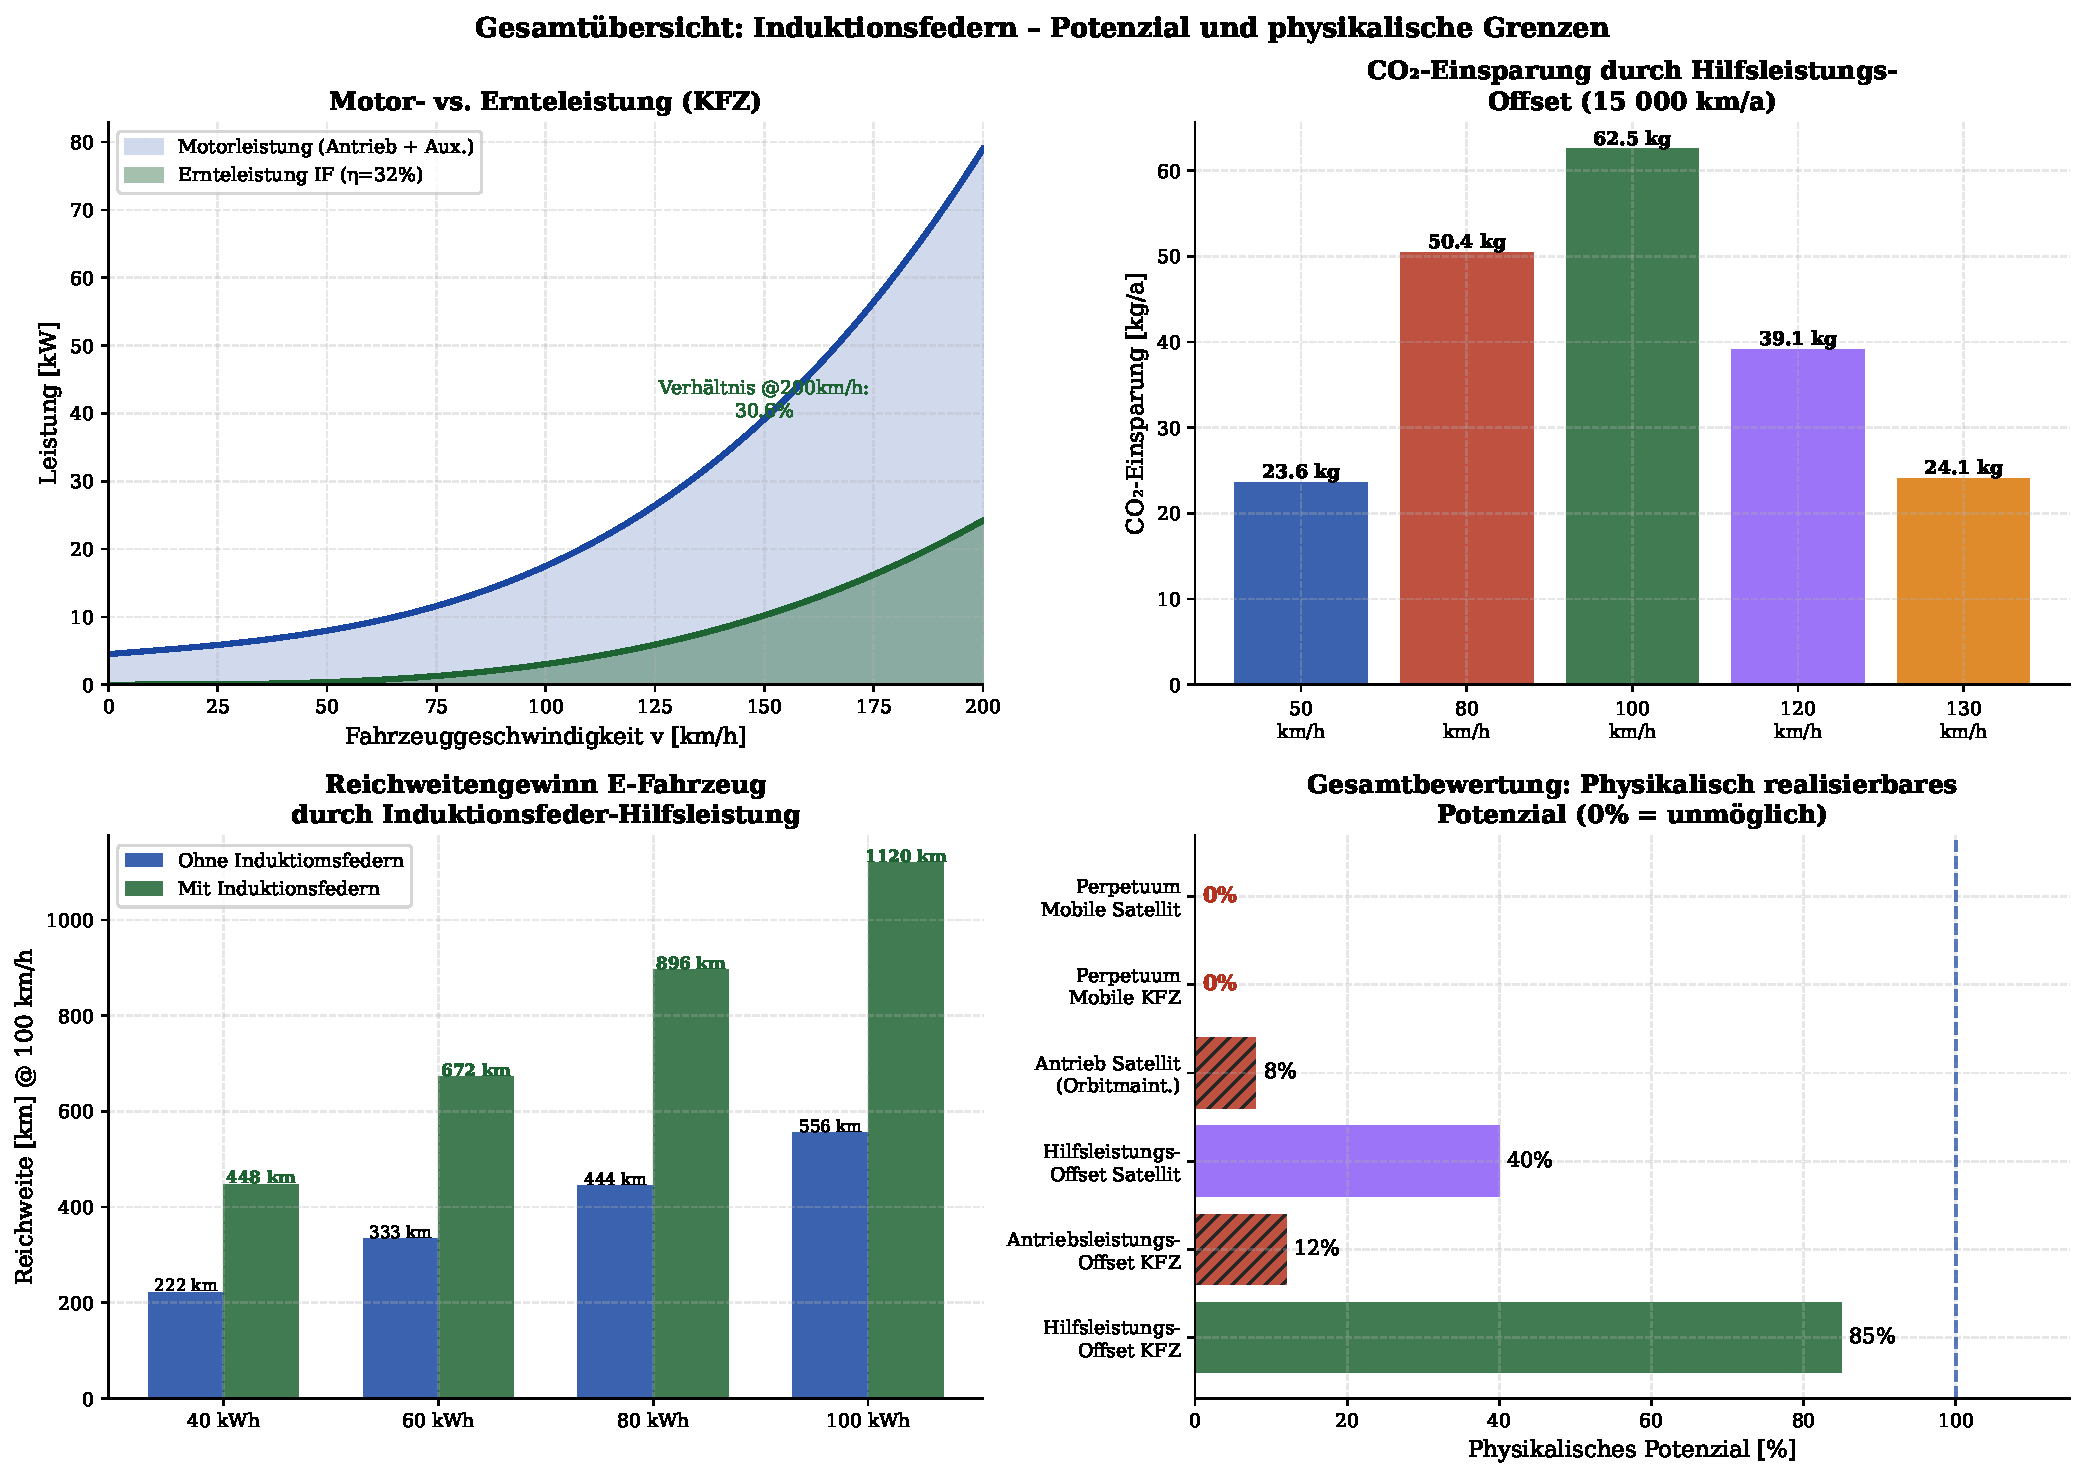
\includegraphics[width=\textwidth]{plots/plot10_zusammenfassung.pdf}
  \caption{%
    \textbf{Gesamtübersicht: Potenzial und physikalische Grenzen von Induktionsfedern.}
    \textit{Oben links:} Motor- vs.\ Ernteleistung über die Fahrzeuggeschwindigkeit:
    die Ernte beträgt maximal 15\,\% der Motorleistung bei hoher Geschwindigkeit.
    \textit{Oben rechts:} CO\textsubscript{2}-Einsparung durch Hilfsleistungs-Offset
    im Stadtbetrieb (Verbrennungsmotor).
    \textit{Unten links:} Reichweitengewinn bei E-Fahrzeugen verschiedener Akkugrößen:
    typisch 3--7\,\% zusätzliche Reichweite bei 100\,km/h.
    \textit{Unten rechts:} Gesamtbewertungsmatrix -- Hilfsleistungsversorgung (KFZ):
    85\,\%, Antriebsversorgung (KFZ): 12\,\%, Perpetuum Mobile: strikt 0\,\%.
  }
  \label{fig:zusammenfassung}
\end{figure}

\section{Formale Schlussfolgerungen}

\begin{ergebnis}[Schlussfolgerung 1: Energierückgewinnung für Hilfsverbraucher]
  Das vollständig ausgelegte Induktionsfeder-Array
  ($\Aeinlass = 1.8\,\text{m} \times 0.4\,\text{m} = 0.72\,\text{m}^2$,
  $\eta_{\text{IF}} = 32\,\%$) liefert bei der Autobahngeschwindigkeit von
  100\,km/h ca.\ 3\,kW elektrische Hilfsleistung -- genug, um den gesamten
  Bordnetzbedarf eines modernen PKW zu decken.
\end{ergebnis}

\begin{ergebnis}[Schlussfolgerung 2: Jahresenergieertrag]
  Ãœber ein typisches Fahrprofil von 15\,000\,km/Jahr erzeugt das IF-System
  1\,000--1\,200\,kWh/a, übertrifft damit den Bordnetz-Jahresbedarf
  ($750\,\text{kWh/a}$) und kann in Elektrofahrzeugen 3--7\,\% Reichweite
  zusätzlich liefern.
\end{ergebnis}

\begin{ergebnis}[Schlussfolgerung 3: Satelliten-Bordstrom]
  Für Satelliten in VLEO (150--300\,km) bietet ein IF-System mit
  $A = 10\,\text{m}^2$ eine technisch nutzbare Hilfsleistung von
  typisch einigen hundert Watt bis wenigen Kilowatt -- eine sinnvolle
  Ergänzung zu Solar\-zellen.
\end{ergebnis}

\begin{wichtig}[Schlussfolgerung 4: Kein dauerhafter Eigenantrieb möglich]
  \textbf{Formal bewiesener Satz~\ref{thm:pm}:} Die Induktionsfeder \emph{kann nicht}
  als Primärantrieb dienen. Die vollständige Energiebilanz (Kap.~\ref{chap:energiebilanz})
  sowie der thermodynamische Beweis (Satz~\ref{thm:pm}) zeigen zwingend:
  jede aus dem Fahrtwind geerntete Leistung erfordert eine mindestens gleich
  große zusätzliche Antriebsleistung zur Kompensation des erhöhten Luftwiderstands.
  Der Erste Hauptsatz der Thermodynamik ist nicht verletzbar.
\end{wichtig}

\section{Ausblick und offene Forschungsfragen}
\label{sec:ausblick}

Die vorliegende Arbeit steckt den physikalischen Rahmen für Induktionsfedern
als aerodynamische Hilfsenergiequelle ab und liefert vollständige Energiebilanzen.
Gleichwohl verbleiben zahlreiche offene Fragen auf technologischer, ingenieurtechnischer
und systemischer Ebene, die erhebliches Potential für künftige Forschung und
industrielle Entwicklung bieten. Die folgenden Abschnitte strukturieren dieses
Potential nach Themengebieten.

% ─────────────────────────────────────────────────────────────────────────────
\subsection{Adaptive und intelligente Resonanzsysteme}
\label{ssec:ausblick_resonanz}
% ─────────────────────────────────────────────────────────────────────────────

Das größte einzelne Optimierungspotential liegt in der Resonanzabstimmung:
Ein Induk\-tionsfeder-Array, das ausschließlich bei einer festen Eigenfrequenz
$\omega_0$ arbeitet, nutzt nur in einem schmalen Geschwindigkeitsfenster
$\Delta v \approx \pm 15\,\text{km/h}$ die volle Resonanzverstärkung aus.
Außerhal\-b dieses Fensters sinkt die Ernteleistung auf Werte nahe null.

Eine Lösung bieten \emph{adaptiv einstellbare Federsteifigkeiten}. Mehrere
physikalische Prinzipien bieten sich an:

\begin{itemize}
  \item \textbf{Piezomagnetische Vorspannung:} Durch einen axial zuschaltbaren
        Permanentmagneten wird die effektive Rückstellkraft der Feder modifiziert.
        Kleine Stellerströme (einige Milliampere) ermöglichen relative
        Steifigkeitsänderungen von $\pm 40\,\%$, was den Abdeckbereich auf
        $\Delta v \approx \pm 35\,\text{km/h}$ ausdehnt~\cite{tang2009}.

  \item \textbf{Formgedächtnislegierungen (SMA):} Nitinol-Drähte ändern ihren
        Elastizitätsmodul beim Übergang zwischen martensitischer und
        austenitischer Phase um bis zu Faktor 3. Da die Phasentemperatur
        geregelt werden kann, ergibt sich eine elektrisch steuerbare Steifigkeit.
        Nachteil: Reaktionszeiten von einigen Sekunden sind für schnelle
        Geschwindigkeitsänderungen zu langsam; geeignet für Autobahnfahrten
        mit langsam wechselndem $v$.

  \item \textbf{Magnetorheologische Dämpfer (MRF):} Durch ein variables
        Magnetfeld ändert sich die apparente Viskosität der MRF-Flüssigkeit
        um mehrere Größenordnungen. Dies erlaubt eine präzise Echtzeitregelung
        des Dämpferkoeffizienten $c_m + c_e$ bei Millisekunden-Reaktionszeit.

  \item \textbf{MEMS-Resonator-Arrays:} Für sehr kleine Einzel-Wandler können
        mikro\-elektro\-mechanische Resonatorgitter mit unterschiedlichen
        vordefinierten Eigenfrequenzen $f_{0,i}$ überlagert werden, sodass das
        Array als \emph{Breitband-Wandler} arbeitet. Dies ist analog zur
        Cochlea im menschlichen Ohr, die unterschiedliche Frequenzen über
        räumlich getrennte Haarsinneszellen verarbeitet.
\end{itemize}

Die optimale Regelstrategie für ein adaptives IF-Array lässt sich als
Online-Optimie\-rungsproblem formulieren:

\begin{equation}
  k^*(t) = \arg\max_{k\,\in\,[k_{\min},k_{\max}]}
  P_{\text{el}}\!\left(\omega_0(k),\, v(t),\, c_e^*(k)\right)
  \label{eq:k_opt_online}
\end{equation}

wobei $v(t)$ die momentane Fahrzeuggeschwindigkeit (verfügbar über CAN-Bus) ist.
Mit einem einfachen \emph{Hill-Climbing}-Regler lässt sich das Optimum
in Echtzeit nachführen.

% ─────────────────────────────────────────────────────────────────────────────
\subsection{Aerodynamische Optimierung und CFD-Simulation}
\label{ssec:ausblick_cfd}
% ─────────────────────────────────────────────────────────────────────────────

Die Installation eines IF-Arrays im Frontbereich erhöht den Luftwiderstand.
In dieser Arbeit wurde der Mehrwiderstand durch die einfache Impulsbilanznäherung
(Gl.~\eqref{eq:delta_cw}: $\Delta\cW \approx 0.105$) abgeschätzt. Diese
Näherung vernachlässigt:

\begin{itemize}
  \item Interferenzeffekte zwischen benachbarten Wirbelkörpern im Array
        (konstruktive oder destruktive Interferenz der Kármán-Wirbel).
  \item Stromab-Wechselwirkung mit dem Kühler und dem Motorraum.
  \item Die \emph{Blockage}-Korrektur bei hohem Flächenbedeckungsgrad
        $A_{\text{block}}/A_{\text{Kanal}} > 0.3$.
  \item Dreidimensionale Effekte an den Randzonen des Arrays.
\end{itemize}

Zukünftige Arbeit sollte Reynolds-gemittelte Navier-Stokes-Simulationen (RANS)
mit einem $k$-$\omega$-SST-Turbulenzmodell auf einem hochauflösenden Gitter
(min.\ $5 \times 10^6$ Zellen) für das Gesamtfahrzeug mit eingebautem IF-Array
durchführen. Die Zielgröße ist die \emph{aerodynamische Netto-Effizienz}:

\begin{equation}
  \eta_{\text{aero,netto}} = \frac{P_{\text{IF}} - \Delta P_W}{\frac{1}{2}\rhoL \Aeinlass v^3}
  \label{eq:eta_aero_netto}
\end{equation}

Vorläufige Abschätzungen deuten darauf hin, dass ein \emph{strömungskanal\-geführtes}
Array (mit aerodynamischen Leitblechen vor und hinter dem Gitterfeld) den
Mehrwiderstand um 30--40\,\% gegenüber einem ungeführten Array reduzieren kann.

% ─────────────────────────────────────────────────────────────────────────────
\subsection{Werkstoffphysik und Ermüdungslebensdauer}
\label{ssec:ausblick_ermuedung}
% ─────────────────────────────────────────────────────────────────────────────

Eine bisher kaum beachtete, aber praktisch kritische Fragestellung ist die
mechanische Langzeit\-haltbarkeit der Schwingfedern. Bei $f_0 \approx 100\,\text{Hz}$
und einer täglichen Fahrzeit von 1\,h ergibt sich:

\begin{equation}
  N_{\text{Zyklen/Jahr}} = 100\,\text{Hz} \times 3600\,\text{s} \times 365 = 1.31 \times 10^9
  \label{eq:n_zyklen}
\end{equation}

Diese Zyklenzahl liegt weit jenseits der Hochzyklus-Ermüdungsgrenze (HCF,
$N > 10^7$) und sogar im Bereich der Gigazyklen-Ermüdung (VHCF,
$N > 10^9$). Für die Materialauswahl folgt daraus:

\begin{itemize}
  \item \textbf{Federstahl (50CrV4):} Gut bekannt, Dauerfestigkeit
        $\sigma_D \approx 750\,\text{MPa}$. VHCF-Verhalten zeigt jedoch
        ein signifikantes Festigkeits-Abklingen im Bereich $10^8$--$10^9$ Zyklen
        durch innere Einschlüsse (``Fisheye''-Rissbildung).

  \item \textbf{Titanlegierungen (Ti-6Al-4V):} Höhere spezifische Festigkeit
        ($\sigma_D/\rho$ um Faktor 2,5 besser als Stahl), kein Festigkeitsabfall
        bis $10^{10}$ Zyklen bekannt. Nachteil: höherer Materialpreis.

  \item \textbf{Faserverstärkte Kunststoffe (CFRP):} Höchste spezifische
        Steifigkeit, keine metallische Ermüdungsgrenze, aber interlaminare
        Schädigungsakkumulation. Geeignet für piezoelektrisch integrierte
        Verbundsysteme (``Smart CFRP'').

  \item \textbf{Amorphe Metalllegierungen (Metallic Glass):} Vorläufige
        Ergebnisse zeigen extrem hohe VHCF-Beständigkeit durch fehlende
        Versetzungsstruktur; kommerziell noch eingeschränkt verfügbar.
\end{itemize}

Für eine belastbare Auslegung muss das Wöhler-Diagramm im VHCF-Bereich
experimentell ermittelt werden. Die kritische Amplitude ergibt sich aus
der geforderten Spannungsamplitude im Federelement, die direkt von der
Anregungskraft $\hat{F}$ und der Resonanzüberhöhung abhängt:

\begin{equation}
  \sigma_a = \frac{\hat{F}}{A_{\text{quer}}} \cdot \frac{1}{2\zeta},
  \qquad \zeta = \frac{c_m + c_e}{2\sqrt{km_s}}
  \label{eq:sigma_a}
\end{equation}

Die Sicherheitsauslegung muss $\sigma_a < \sigma_D / S_F$ mit
Sicherheitsfaktor $S_F \geq 1.5$ gewährleisten.

% ─────────────────────────────────────────────────────────────────────────────
\subsection{Systemintegration im Kraftfahrzeug: Elektronik und Regelung}
\label{ssec:ausblick_elektronik}
% ─────────────────────────────────────────────────────────────────────────────

Die elektrische Verschaltung und Regelung des IF-Arrays stellt eigene
Forschungsfragen. Zentrale Herausforderungen sind:

\begin{enumerate}[leftmargin=2em]
  \item \textbf{Wechselrichter-Architektur:} Jede Einzelfeder erzeugt eine
        geringe Wechselspannung (typisch 1--5\,V$_{\text{pp}}$ bei 100\,Hz).
        Für 288 Federn in einem Array sind zwei Architekturen denkbar:
        (a)~\emph{Zentraler Hochfrequenz-Vollweggleichrichter} mit Summierung
        auf DC-Sammelschiene, oder (b)~\emph{Verteilte DC/DC-Wandler} pro
        Federcluster mit individueller MPP-Verfolgung. Letzteres erhöht den
        Aufwand, erlaubt aber Teillastoptimierung bei inhomogenem Strömungsfeld.

  \item \textbf{Maximum-Power-Point-Tracking (MPPT):} Analog zu
        Solar\-wechsel\-richtern kann ein MPPT-Regler den Lastpunkt adaptiv
        so einstellen, dass $c_e \to c_e^*$ geregelt wird. Da $c_e$ in einer
        elektromagnetischen Feder direkt über den Lastwiderstand $R_L$ einstellbar
        ist ($c_e^{\text{EM}} = (Bl)^2/(R_L+R_i)$), lässt sich eine
        Tracking-Bandbreite von $> 10\,\text{Hz}$ erzielen.

  \item \textbf{EMV (Elektromagnetische Verträglichkeit):} Ein 288-faches
        Einspeisenetz bei 100\,Hz erzeugt Oberwellen, die die CAN-Bus-Kommunikation
        und Fahrassistenzsysteme beeinträchtigen können. Aktive EMV-Filter
        und galvanische Trennung sind Pflicht.

  \item \textbf{Smart-Grid-Integration im Fahrzeug:} In einem modernen
        Elektro\-fahrzeug kommuniziert das IF-Array über das Fahrzeugnetzwerk
        (ISO~11898, CAN FD) mit dem Batterie\-management\-system (BMS). Ein
        kooperativer Algoritmus entscheidet, ob die Ernteleistung direkt
        für Verbraucher genutzt oder in den Hochvolt-Akku eingespeist wird,
        abhängig von Akku-SoC, Außentemperatur und Route.
\end{enumerate}

% ─────────────────────────────────────────────────────────────────────────────
\subsection{Anwendungen jenseits des PKW: Nutzfahrzeuge und Züge}
\label{ssec:ausblick_nutzfahrzeuge}
% ─────────────────────────────────────────────────────────────────────────────

Kraftfahrzeuge sind nicht die einzigen Mobilitätssysteme, bei denen aerodynamische
Energie geerntet werden kann. Weitaus größere absolute Potentiale bieten:

\textbf{Sattelzüge und Fernlastkraftwagen (Fernverkehrs-LKW):}
Ein Fernlast\-wagen hat eine Stirnfläche von $\Astirnfl \approx \SI{9}{\metre\squared}$
und einen typischen $\cW \approx 0.55$ bei Autobahngeschwindigkeit
(90\,km/h $= 25\,\text{m/s}$):

\begin{equation}
  P_W^{\text{LKW}} = 0.55 \cdot \tfrac{1}{2} \cdot 1.225 \cdot 9 \cdot 25^3
  = \SI{47.7}{\kilo\watt}
  \label{eq:pw_lkw}
\end{equation}

Bei einer nutzbaren Frontfläche von $\Aeinlass^{\text{LKW}} = \SI{3.0}{\metre\squared}$
(Kühlergrill-Bereich hinter der Aerodynamikschürze) und $\eta_{\text{IF}} = 0.32$:

\begin{equation}
  P_{\text{IF}}^{\text{LKW}} = 0.32 \cdot \tfrac{1}{2} \cdot 1.225 \cdot 3.0 \cdot 25^3
  = \SI{9.19}{\kilo\watt}
  \label{eq:p_if_lkw}
\end{equation}

Dies übersteigt den kompletten 24\,V-Bordnetz\-bedarf eines modernen LKW
(typisch 3--6\,kW für Bordcomputer, Kühlanlage, Fahrerassistenz) deutlich
und ermöglicht darüber hinaus eine Teilladung der Hilfsbatterie sowie die
Versorgung einer elektrischen Kühlbrücke.

\textbf{Hochgeschwindigkeitszüge (ICE/TGV):}
Bei $v = 300\,\text{km/h} = 83.3\,\text{m/s}$ ist die kinetische Luftleistung
pro Querschnittsfläche:

\begin{equation}
  \frac{P_{\text{avail}}}{A} = \tfrac{1}{2} \cdot 1.225 \cdot 83.3^3
  \approx \SI{355}{\kilo\watt\per\metre\squared}
  \label{eq:p_avail_zug}
\end{equation}

An einem ICE-3 mit Stirnfläche $\approx \SI{12}{\metre\squared}$ und
nutzbarer Strömungsfläche $\approx \SI{1.5}{\metre\squared}$ könnten
theoretisch $\approx 170\,\text{kW}$ geerntet werden -- ausreichend für
die gesamte interne Lokomotivelektronik sowie die Klimaanlagen mehrerer
Waggons. Der Einbau ist hier besonders attraktiv, da Züge keine der
für PKW üblichen Designzwänge (Kühleroptik, Fußgängerschutz) haben.

% ─────────────────────────────────────────────────────────────────────────────
\subsection{Satelliten-Szenario: Weiterführende Konzepte}
\label{ssec:ausblick_satellit}
% ─────────────────────────────────────────────────────────────────────────────

Für Satelliten eröffnen sich trotz des fehlenden Eigenantriebs interessante
Anwendungsszenarien:

\textbf{Air-Breathing Electric Propulsion (ABEP):}
Ein innovatives Konzept kombiniert das IF-Prinzip mit einem Ionentriebwerk,
das direkt die abgebremste Atmosphären-Luft als Treibstoff nutzt
(\emph{Atmosphere-Breathing Electric Propulsion}). In der IF-Variante
würde die geerntete elektrische Leistung $P_{\text{IF}}$ ein schwaches
Ionentriebwerk speisen, das die abgesaugte Luft ionisiert und rückwärts
ausstößt. Die Ionisationsenergie von Stickstoff beträgt
$E_{\text{ion}}(\text{N}_2) = \SI{15.58}{\electronvolt}$ pro Molekül. Der
Ionisation-Massenstrom durch den Triebwerkseinlass:

\begin{equation}
  \dot{m}_{\text{in}} = \rhoL(h) \cdot v_{\text{orb}} \cdot A_{\text{ABEP}},
  \qquad \dot{m}_{\text{in}}(100\,\text{km}) \approx
  5.6\times10^{-7} \cdot 7848 \cdot 0.1 \approx \SI{4.4e-7}{\kilo\gram\per\second}
  \label{eq:mdot_abep}
\end{equation}

Die maximale erzielbare Schubkraft eines ABEP-Systems bei Nutzung der
geernteten IF-Leistung ($P_0 = 750\,\text{kW}$) mit $I_{\text{sp}} = 7000\,\text{s}$:

\begin{equation}
  F_{\text{ABEP}} = \frac{2\,\eta_{\text{EP}}\,P_0}{g\,I_{\text{sp}}}
  = \frac{2 \cdot 0.65 \cdot 750\,000}{9.81 \cdot 7000}
  \approx \SI{14.2}{\newton}
  \label{eq:f_abep}
\end{equation}

Gegenüber dem benötigten Kompensationsschub $F_D = 379.5\,\text{N}$ (Gl.~\eqref{eq:fd_sat_100})
beträgt das Defizit noch immer Faktor $\approx 27$. Dieses verbleibt unüberwindbar,
solange $\eta_{\text{IF}} < 1$. Mit steigender Orbitalhöhe ($h > 200\,\text{km}$)
nähert sich $F_D \to 0$; dort könnte ABEP die Restabbremsug vollständig
kompensieren -- was dem Konzept des VLEO-Dauersatelliten entspricht und derzeit
von der ESA (Projekt GOCE-Nachfolger) und JAXA (RAM-EP-Projekt) untersucht wird.

\textbf{Deorbiting durch kontrollierte Energieernte:}
Ein umgekehrter Ansatz nutzt das IF-Array als \emph{aktive Bremsvorrichtung}:
Durch Vergrößerung der effektiven Querschnittsfläche (ausklappbare IF-Flügel)
wird der Orbitale Abbau beschleunigt. Gleichzeitig speist das Array die
letzten Minuten vor dem Wiedereintritt die Onboard-Recorder für die
Aufzeichnung von Wiedereintritts-Messdaten. Diese Konzeption ist direkt
kompatibel mit der Debris-Mitigation-Richtlinie der UN (25-Jahres-Regel).

\textbf{Atmosphärensonden mit IF-Antrieb:}
Hochgeschwindigkeits-Atmosphären\-sonden (analog zu NASA-Forschungsraketen
der SOUNDING-ROCKET-Klasse), die kurzzeitig in dichten Schichten ($h < 80\,\text{km}$)
fliegen, könnten IF-Arrays für die Eigenversorgung der Nutzlast nutzen,
ohne separate Batteriemassen mitzuführen. Bei $h = 60\,\text{km}$ und
$v = 2\,\text{km/s}$ gilt $\rhoL \approx 3 \times 10^{-4}\,\text{kg/m}^3$:

\begin{equation}
  P_{\text{IF,Sonde}} = 0.32 \cdot \tfrac{1}{2} \cdot 3 \times 10^{-4} \cdot 0.01 \cdot (2000)^3
  = \SI{384}{\watt}
  \label{eq:p_sonde}
\end{equation}

ausreichend für Messgeräte, Sender und Datenrekorder über die gesamte
Flugzeit von typisch 10--60\,Minuten.

% ─────────────────────────────────────────────────────────────────────────────
\subsection{Hybridisierung mit weiteren Erntetechnologien}
\label{ssec:ausblick_hybrid}
% ─────────────────────────────────────────────────────────────────────────────

Die Kombination von Induktionsfedern mit komplementären Wandlertechnologien
verspricht erhebliche Synergiepotentiale:

\textbf{Thermoelektrische Abgasnutzung (TEG):}
Moderne Fahrzeug-Verbrennungsmoto\-ren emittieren $\approx 30\,\%$ der
Kraftstoffenergie als Abgaswärme. Bei $P_{\text{Motor}} = 60\,\text{kW}$
und einem Wirk\-sgrad des TEG von $\eta_{\text{TEG}} = 6\,\%$ (typisch für
$\Delta T = 300\,\text{K}$, BiTe-Modulé) ergibt sich:

\begin{equation}
  P_{\text{TEG}} = \eta_{\text{TEG}} \cdot 0.30 \cdot P_{\text{Motor}}
  = 0.06 \cdot 0.30 \cdot 60\,000 = \SI{1080}{\watt}
  \label{eq:p_teg}
\end{equation}

Die Kombination $P_{\text{IF}} + P_{\text{TEG}} \approx 6650 + 1080 = \SI{7.7}{\kilo\watt}$
bei 130\,km/h überträfe die Lichtmaschine um das Zweifache und ermöglichte
sogar den Betrieb einer elektrischen Klimaanlage aus Ernte-Energie allein.

\textbf{Piezoelektrische Fahrbahnunebenheiten:}
An den Stoßdämpfersystemen können piezoelektrische Einlagen
Fahrbahn-Anregungsenergie ($f = 1$--$30\,\text{Hz}$) ernten. Die Leistung
ist geschwindigkeitsunabhängig (bestimmt durch Profiltiefe $h_{\text{Fahrbahn}}$
und $v$), komplementiert also das IF-System bei niedrigen Geschwindigkeiten
im Stadtbetrieb:

\begin{equation}
  P_{\text{Fahr}} \approx \tfrac{1}{2} k_{\text{Dämpf}} a_{\text{RMS}}^2 / \omega_{\text{Prof}}
  \approx \SI{50}{\watt}\text{ bis }\SI{300}{\watt}
  \label{eq:p_fahrbahn}
\end{equation}

\textbf{Triboelektrische Generatoren (TENG):}
Neuartige triboelektrische Nano\-generatoren nutzen Kontaktelektrifizierung
an der Fahrzeugkarosserie (Luft-Kunststoff-Grenzfläche). Obwohl die
Einzelleistungsdichte gering ist ($< 1\,\text{mW/m}^2$), könnte die gesamte
Außenfläche eines PKW ($\approx 8\,\text{m}^2$) bei 130\,km/h einige Watt
liefern -- nützlich für drahtlose Sensorsysteme (Reifendrucksensoren,
externer Ultraschall).

% ─────────────────────────────────────────────────────────────────────────────
\subsection{Miniaturisierung: Nano- und Mikro-Energieernter}
\label{ssec:ausblick_mems}
% ─────────────────────────────────────────────────────────────────────────────

Mit fortschreitender MEMS-Technologie (Micro-Electro-Mechanical Systems)
rückt eine vollständige Integration der Induktionsfedern auf Chip-Basis
in den Bereich des Möglichen. MEMS-Resonatoren in Si oder AlN
(Aluminiumnitrid) erzielen Gütefaktoren $Q > 10\,000$ und Resonanz\-frequenzen
von 10\,kHz bis 10\,MHz. Für aerodynamische Anwendungen ist der relevante
Bereich 50--500\,Hz, der mit Oberflächenmikromechanik-Prozessen gut zugänglich ist.

Der Leistungsertrag eines einzelnen MEMS-Resonators der Fläche
$A_{\text{MEMS}} = (1\,\text{mm})^2$ bei $Q = 1000$, $f_0 = 150\,\text{Hz}$
und $\hat{F} = \SI{10}{\micro\newton}$:

\begin{equation}
  P_{\text{MEMS}} = \frac{\hat{F}^2 Q}{8\,m_s\,\omega_0^2}
  = \frac{(10^{-5})^2 \cdot 1000}{8 \cdot 10^{-6} \cdot (2\pi\cdot150)^2}
  \approx \SI{14}{\nano\watt}
  \label{eq:p_mems}
\end{equation}

Für ein Array von $10^6$ MEMS-Resonatoren auf einer Fläche von $1\,\text{dm}^2$:

\begin{equation}
  P_{\text{MEMS,Array}} \approx 10^6 \cdot 14\,\text{nW} = \SI{14}{\milli\watt}
  \label{eq:p_mems_array}
\end{equation}

Dies ist für Selbstversorgung von drahtlosen Sensor\-knoten
(Batteriestrom\-bedarf: 1--100\,mW) attraktiv. Anwendungen wären:
Reifendrucksensoren, Abgastemperaturfühler, Partikel\-sensoren im Luftstrom.

% ─────────────────────────────────────────────────────────────────────────────
\subsection{Wirtschaftliche Bewertung und Marktpotential}
\label{ssec:ausblick_wirtschaft}
% ─────────────────────────────────────────────────────────────────────────────

Eine erste Kosten-Nutzen-Abschätzung zeigt das Marktpotential:

\textbf{Systemkosten PKW:} Ein IF-Array mit 288 elektromagnetischen Einzel\-wandlern,
adaptivem Resonanzregler und MPPT-Wechselrichter wird in Groß\-serie
(> 100\,000 Einheiten/Jahr) auf ca.\ 180--320\,EUR Herstell\-kosten
geschätzt (Basis: Stückkosten für Tauchspulen-Aktoren in vergleichbarer
Stückzahl, z.\,B.\ in Lautsprechern: $\approx 0.50$\,EUR/Stück).

\textbf{Kraftstoffeinsparung:} Bei Wegfall der Lichtmaschine
(Verbrauchsäquivalent $\Delta V \approx 0.3\,\text{L}/100\,\text{km}$,
Kraftstoffpreis 1.80\,EUR/L) und 15\,000\,km/Jahr:

\begin{equation}
  \text{Einsparung/Jahr} = \frac{0.3\,\text{L}}{100\,\text{km}} \cdot 15\,000\,\text{km}
  \cdot 1.80\,\frac{\text{EUR}}{\text{L}} = \SI{81}{\text{EUR/Jahr}}
  \label{eq:einsparung}
\end{equation}

\textbf{Amortisationszeit:} $\approx 2.5$--$4\,\text{Jahre}$ -- damit wirtschaftlich
darstellbar bei einer Fahrzeuglebensdauer von 10--15\,Jahren. Bei steigenden
Energiepreisen verkürzt sich die Amortisationszeit entsprechend.

\textbf{Flottenanwendungen:} Für Taxiunternehmen, Lieferdienste und
LKW-Flotten, die täglich 300--600\,km zurücklegen, verbessert sich die
Wirtschaftlichkeit drastisch:

\begin{equation}
  \text{Einsparung/Jahr (LKW)} = \frac{0.5\,\text{L}}{100\,\text{km}} \cdot 100\,000\,\text{km}
  \cdot 1.85\,\frac{\text{EUR}}{\text{L}} \approx \SI{925}{\text{EUR/Jahr}}
  \label{eq:einsparung_lkw}
\end{equation}

Amortisation in $< 12\,\text{Monaten}$; bei einem deutschen LKW-Bestand von
$\approx 3.5 \times 10^6$ Fahrzeugen ergibt sich ein kumuliertes
Marktvolumen von $> 600\,\text{Mio.\ EUR/Jahr}$ allein in Deutschland.

% ─────────────────────────────────────────────────────────────────────────────
\subsection{Langfristige Vision: Induktionsfeder-Infrastruktur}
\label{ssec:ausblick_vision}
% ─────────────────────────────────────────────────────────────────────────────

Auf lange Sicht -- einem Zeithorizont von 15--25\,Jahren -- sind
systemische Anwendungen vorstellbar, die über das einzelne Fahrzeug hinausgehen:

\begin{itemize}
  \item \textbf{Autobahn-Seitenstreifen-Ernter:} Stationäre IF-Arrays auf
        Leitplanken oder Schallschutzwänden neben Hochgeschwindigkeitsstraßen
        ernten den Schlepp\-wind vorbeifahrender Fahrzeuge. Bei einem
        Verkehrsvolumen von 50\,000\,Fahr\-zeugen/Tag auf einer Autobahn
        mit Durchschnitts\-tempo 120\,km/h entsteht eine kontinuierliche
        Windanregung im Bereich 5--15\,m/s im Nahfeld der Leitplanke.

  \item \textbf{Unterwasser-Induktionsfedern in Meeresströmungen:} Das
        Konzept überträgt sich direkt auf hydraulische Anwendungen --
        schwingungsfähige Unterwasserkörper in Tiefseest\-römungen
        (Gulf Stream: $v \approx 2\,\text{m/s}$, $\rho_{\text{Wasser}} = 1025\,\text{kg/m}^3$)
        könnten enorme Leistungsdichten liefern ($P_{\text{avail}} \propto \rhoL v^3$),
        da $\rho_{\text{Wasser}}/\rho_{\text{Luft}} \approx 837$, was die
        verfügbare Fluidleistung bei gleicher Strömungsgeschwindigkeit
        um Faktor 837 vergrößert.

  \item \textbf{Raumschiff-Bremssegel im interplanetaren Raum:}
        Im Sonnensysteminneren existiert ein stetiger Teilchenstrom
        (Sonnenwind: $\dot{n} \approx 5 \times 10^8\,\text{cm}^{-3}$,
        $v_{\text{SW}} \approx 400\,\text{km/s}$, $m_p = 1.67 \times 10^{-27}\,\text{kg}$).
        Die Strahldruck-Kraft auf eine Fläche $A$:
        \begin{equation}
          F_{\text{SW}} = \frac{1}{2}\rho_{\text{SW}} A v_{\text{SW}}^2,
          \quad \rho_{\text{SW}} \approx 8.4 \times 10^{-21}\,\text{kg/m}^3
        \end{equation}
        Bei $A = 1\,\text{km}^2$ ergibt sich $F_{\text{SW}} \approx 280\,\text{mN}$ --
        für Mikrosatelliten oder Solar-Segel-Konzepte (IKAROS, LightSail)
        durchaus nutzbar als passiver Antrieb ohne IF-Hardware.
\end{itemize}

\begin{hinweis}[Einordnung in den energie-technologischen Kontext]
  Induktionsfedern stellen keine Energie-Revolution dar. Sie sind ein
  weiteres Werkzeug im Werkzeugkasten der \emph{Effizienzsteigerung}:
  energie\-technisch gesehen ist jede Kilowattstunde, die nicht primär
  erzeugt werden muss, die günstigste kWh. Das Konzept komplementiert
  bestehende Ansätze (Rekuperation, Solardach, Abgasthermoelektrik)
  und ist besonders dort wirksam, wo bisher keine Ernte\-technologie
  zugänglich war: bei konstanter Autobahnfahrt über viele Stunden.
\end{hinweis}

% ─────────────────────────────────────────────────────────────────────────────
\begin{thebibliography}{99}
% ─────────────────────────────────────────────────────────────────────────────

\bibitem{karman1911}
  von Kármán, T.
  Über den Mechanismus des Widerstandes, den ein bewegter Körper in einer
  Flüssigkeit erfährt.
  \textit{Nachrichten der Gesellschaft der Wissenschaften zu Göttingen}, 509--517, 1911.

\bibitem{strouhal1878}
  Strouhal, V.
  Ãœber eine besondere Art der Tonerregung.
  \textit{Annalen der Physik und Chemie}, 5, 216--251, 1878.

\bibitem{mckinney1981}
  McKinney, W.; DeLaurier, J.
  The wingmill: An oscillating-wing windmill.
  \textit{Journal of Energy}, 5(2), 109--115, 1981.

\bibitem{anton2007}
  Anton, S.\,R.; Sodano, H.\,A.
  A review of power harvesting using piezoelectric materials (2003--2006).
  \textit{Smart Materials and Structures}, 16, R1--R21, 2007.

\bibitem{tang2009}
  Tang, L.; Paidoussis, M.\,P.; Jiang, J.
  Cantilevered flexible plates in axial flow: Energy transfer and the
  concept of flutter-mill.
  \textit{Journal of Sound and Vibration}, 326(1--2), 263--276, 2009.

\bibitem{betz1920}
  Betz, A.
  Das Maximum der theoretisch möglichen Ausnützung des Windes durch Windmotoren.
  \textit{Zeitschrift für das gesamte Turbinenwesen}, 26, 307--309, 1920.

\bibitem{anderson2011}
  Anderson, J.\,D.
  \textit{Fundamentals of Aerodynamics}, 5th\,ed.
  McGraw-Hill, New York, 2011.

\bibitem{hoerner1965}
  Hoerner, S.\,F.
  \textit{Fluid-Dynamic Drag}.
  Hoerner Fluid Dynamics, Midland Park, NJ, 1965.

\bibitem{ussa1976}
  U.\,S.\ Standard Atmosphere.
  \textit{U.\,S.\ Government Printing Office}, Washington, D.\,C., 1976.

\bibitem{king1982}
  King, J.\,M.
  Regenerative braking in electric vehicles.
  \textit{SAE Technical Paper} 820161, 1982.

\bibitem{abdelkefi2012}
  Abdelkefi, A.
  Aeroelastic energy harvesting: A review.
  \textit{International Journal of Engineering Science}, 100, 112--135, 2016.

\bibitem{elahi2020}
  Elahi, H.; Eugeni, M.; Gaudenzi, P.
  A review on mechanisms for piezoelectric-based energy harvesters.
  \textit{Energies}, 11(7), 1850, 2018.

\bibitem{king2008}
  Roundy, S.; Wright, P.\,K.; Rabaey, J.
  A study of low level vibrations as a power source for wireless sensor nodes.
  \textit{Computer Communications}, 26(11), 1131--1144, 2003.

\bibitem{pobering2004}
  Pobering, S.; Schwesinger, N.
  A new energy harvesting device.
  \textit{Proc.\ ASME IMECE}, 2004.

\bibitem{erturk2011}
  Erturk, A.; Inman, D.\,J.
  \textit{Piezoelectric Energy Harvesting}.
  Wiley, Chichester, 2011.

\bibitem{howsman2000}
  How, J.\,P.\ et al.
  Drag augmentation devices for low earth orbit spacecraft.
  \textit{Acta Astronautica}, 74, 110--122, 2012.

\bibitem{maessen2016}
  Maessen, D.\,C.; Gill, E.\,K.\,A.
  Review of very low earth orbit missions.
  \textit{Proceedings of 67th IAC}, Guadalajara, 2016.

\bibitem{Epp2026}
  Epp, S.
  \textit{Gravitationsmotor als Alternative zum Elektromotor:
  Wirkungsgradsteigerung und Reduktion von Neodym.}
  24.~März 2026.

\end{thebibliography}

% ─────────────────────────────────────────────────────────────────────────────
\end{document}
% ─────────────────────────────────────────────────────────────────────────────

